%%%%%%%%%%%%%%%%%%%%%%%%%%%%%%%%%%%%%%%%%%%%%%%%%%%%%%%%%%%%%%%%%%%%%%%%%%%%%%%%
%
%   全国大学生数学建模竞赛 LaTeX 论文模板 (2025版)
%
%   版本: 2.1
%   作者: AI & Human Collaboration
%   更新日期: 2024-08-15
%
%   本模板严格遵循2025年全国大学生数学建模竞赛论文格式规范和AI工具使用规定。
%   特点:
%   1.  符合最新的AI工具使用声明要求。
%   2.  A4页面，2.5cm页边距，页脚中部页码。
%   3.  电子版以摘要页为首页，无目录。
%   4.  包含完整的论文结构：摘要、正文、参考文献、附录。
%   5.  附录部分包含支撑材料列表和代码展示的标准格式。
%   6.  使用 ctex 宏包，完美支持中文。
%   7.  预置了常用的数学、图形、表格、代码等宏包。
%
%%%%%%%%%%%%%%%%%%%%%%%%%%%%%%%%%%%%%%%%%%%%%%%%%%%%%%%%%%%%%%%%%%%%%%%%%%%%%%%%

\documentclass[a4paper]{ctexart}

%--------------------------------------------------------------------------
%   宏包导入
%--------------------------------------------------------------------------
\usepackage{amsmath, amssymb, amsfonts} % AMS 数学宏包
\usepackage[a4paper, margin=2.5cm]{geometry} % 设置页边距
\usepackage{graphicx}          % 插入图片
\usepackage{booktabs}          % 专业三线表
\usepackage{caption}           % 自定义图表标题
\usepackage{fancyhdr}          % 设置页眉页脚
\usepackage{listings}          % 插入代码
\usepackage{color}             % 支持颜色
\usepackage{hyperref}          % 创建超链接 (建议最终提交时移除或设置为全黑)
\usepackage[numbers, sort&compress]{gbt7714}
\usepackage{enumitem}
\usepackage{siunitx}
\usepackage{amsmath}
\usepackage{subcaption}
\usepackage{svg}
\usepackage{float}

% 图片资源路径（图片统一存放于 img/，源代码存放于 code/）
\graphicspath{{img/}}
\svgpath{{img/}}

% 兼容性：BibTeX 在大写化作者名时把 \i（无点小写 i）转成未定义的 \I，
% 这里补充其定义（大写 I），使参考文献 \'\I 渲染为 Í，避免编译中断
\providecommand{\I}{I}

%--------------------------------------------------------------------------
%   全局格式设置
%--------------------------------------------------------------------------
% 设置图表标题格式
\captionsetup{labelsep=space, font=small, justification=centering}

% 设置页眉页脚
\pagestyle{fancy}
\fancyhf{} % 清空所有页眉页脚
\fancyfoot[C]{\thepage} % 页脚中部显示页码
\renewcommand{\headrulewidth}{0pt} % 去掉页眉横线

% 设置超链接颜色 (保持打印版和电子版观感一致)
\hypersetup{
    colorlinks=true,
    linkcolor=black,
    citecolor=black,
    urlcolor=black,
}

% 设置代码块 (listings) 风格
\definecolor{codegreen}{rgb}{0,0.6,0}
\definecolor{codegray}{rgb}{0.5,0.5,0.5}
\definecolor{codepurple}{rgb}{0.58,0,0.82}
\definecolor{backcolour}{rgb}{0.95,0.95,0.92}

\lstdefinestyle{mystyle}{
    backgroundcolor=\color{backcolour},   
    commentstyle=\color{codegreen},
    keywordstyle=\color{magenta},
    numberstyle=\tiny\color{codegray},
    stringstyle=\color{codepurple},
    basicstyle=\fontfamily{consolas}\footnotesize, % 推荐使用 Consolas 字体
    breakatwhitespace=false,         
    breaklines=true,                 
    captionpos=b,                    
    keepspaces=true,                 
    numbers=left,                    
    numbersep=5pt,                  
    showspaces=false,                
    showstringspaces=false,
    showtabs=false,                  
    tabsize=2,
    frame=single,
    rulecolor=\color{black},
    extendedchars=true, % 支持非 ASCII 字符
    inputencoding=utf8, % 支持 UTF-8 编码
    literate={-}{-}1 % 解决代码中减号显示问题
}
\lstset{style=mystyle}

%--------------------------------------------------------------------------
%   文档开始
%--------------------------------------------------------------------------
\begin{document}

%==========================================================================
%   摘要页 (电子版论文的第一页)
%==========================================================================
\begin{center}
    \vspace*{0.2cm} % 调整标题与顶部的距离
    {\Large\bfseries 基于联合物理色散模型与先进信号处理方法测定碳化硅外延层厚度} % 论文标题
    \vspace*{1cm}
    
    {\Large\bfseries 摘\quad 要}
\end{center}

\thispagestyle{fancy} % 确保摘要页也有页码 "1"


本文针对红外干涉法测量半导体外延层厚度问题，建立了基于物理原理的双光束及多光束数学模型。我们为碳化硅和硅两种材料分别构建了针对性的折射率模型，并设计了相应的外延层厚度求解算法。通过对光谱数据进行分析，我们成功求解出其外延层厚度，并基于结果揭示了样品的物理性质及多光束干涉效应的影响。

\noindent \textbf{针对问题一}，为精确确定碳化硅外延层的厚度，我们建立了两个核心模型。一：采用基于\textbf{菲涅尔方程的双光束干涉理论}来描述光波在“空气-外延层-衬底”三层结构中的干涉过程；二：针对碳化硅的色散特性，我们引入了能同时描述晶格振动与自由载流子影响的\textbf{洛伦兹-德鲁德（Lorentz-Drude）色散模型}。

\noindent \textbf{针对问题二}，我们采用问题一建立的数学模型，通过拟合实验光谱来反演样品七个未知的物理参数。为此，我们设计了\textbf{“差分进化全局搜索”与“L-BFGS-B局部优化”}相结合的算法，实现了对两组光谱数据的同步拟合。模型取得了极佳的拟合优度，决定系数\textbf{R²分别高达0.9967和0.9948}，最终确定外延层厚度为\textbf{7.413 µm}。基于拟合出的参数，我们发现外延层与衬底折射率高度匹配，从而证明了在该体系中多光束干涉效应可以忽略。最后，我们根据残差分析确认了结果的可靠性。

\noindent \textbf{针对问题三}，我们首先推导了产生多光束干涉的必要条件：相干性、界面反射率与材料吸收、以及几何均匀性,并分析出多光束干涉将有效提高硅晶圆片外延层厚度计算精度。然后，我们再对附件3和附件4的硅晶圆片光谱数据进行分析，通过干涉条纹的非对称性，先定性判断发生多光束干涉。针对硅的特性，我们采用\textbf{塞尔迈耶方程}描述折射率，并通过\textbf{干涉极值点解析法}，识别光谱极值点位置并反解出厚度，计算出硅晶圆片厚度为\textbf{3.751 µm}。为了定量证明发生了多光束干涉，我们通过反射率、介质折射率反推出衬底折射率，利用菲涅尔公式，定量计算出了各级反射光振幅、光谱精细度（$F\approx 2.7>2$）等数值，严谨证明了\textbf{多光束干涉效应的存在}。然而，我们发现干涉极值点法存在局限性：在高波数区，由于信号衰减，极值点定位精度下降。为克服此问题并利用全谱信息，我们引入了\textbf{基于色散矫正的傅里叶变换（FFT）频率分析法},并创新性地引入\textbf{坐标变换}来解决硅的色散现象导致的干涉信号的非周期性，将信号转化为一个在新坐标域中周期性与厚度严格对应的信号，利用FFT从光谱数据中提取出基频，得到更准确的硅晶圆片厚度结果\textbf{d = 3.595 µm}。

 此外，为了判定多光束干涉对问题二碳化硅外延层计算精度的影响，我们运用问题三推导的多光束干涉判据进行分析，最终确认\textbf{碳化硅无需考虑多光束干涉}，因此问题二采用的双光束干涉模型是充分且精确的。

综上所述，本文所建模型经过物理严格推导且针对性强，使用的算法精度高，准确计算了碳化硅和硅外延层的厚度测定，还通过灵敏度与稳定性检验证明了模型的稳健性，可为相关领域的精确测量提供科学依据。

\vspace{1cm} % 摘要与关键词之间的距离

\noindent {\bfseries 关键词：} 外延层厚度；红外干涉光谱；洛伦兹-德鲁德模型；差分进化；L-BFGS-B；塞尔迈耶模型；傅里叶变换；色散校正

\newpage % 摘要结束后换页

%==========================================================================
%   正文部分 (从此页开始)
%==========================================================================
\section{问题背景}
碳化硅作为一种新兴的第三代半导体材料，以其优越的综合性能表现正在受到越来越多的关注。碳化硅外延层的厚度是外延材料的关键参数之一，对器件性能有重要影响。因此，制定一套科学、准确、可靠的碳化硅外延层厚度测试标准显得尤为重要。红外干涉法是外延层厚度测量的无损伤测量方法，可根据红外光谱的波长、外延层的折射率和红外光的入射角等参数确定外延层的厚度。针对红外干涉法测量外延层长度建立模型后，可以确定反射光谱与外延层厚度等参数之间的关系，可以在实际生产中用于评估外延层的质量和性能是否符合应用要求、最终产品的可靠性、性能和良率。
\section{问题重述}
\begin{itemize}
    \item 问题一：红外光入射到外延层后，一部分从外延层表面反射出来，另一部分从衬底表面反射回来，这两束光在一定条件下会产生干涉条纹。问题一限制了条件，只需考虑外延层和衬底界面只有一次反射、透射所产生的干涉条纹的情形，要求建立确定外延层厚度的数学模型。问题还明确指出外延层的折射率不是常数，它与掺杂载流子的浓度、红外光谱的波长等参数有关。
    \item 问题二：该问题要求根据问题一建立的数学模型，设计确定外延层厚度的算法，基于附件给定的实测数据，计算碳化硅晶圆片外延层的厚度。
    \item 问题三：问题增加了光波可以在外延层界面和衬底界面产生多次反射和透射的条件，需要推导产生多光束干涉的必要条件，并且据此判断硅晶圆片是否产生了多光束干涉，以此为基础重新建立计算外延层厚度的数学模型，设计确定外延层厚度的算法，并基于附件给定的实测数据，计算硅晶圆片外延层的厚度，最后分析多光束干涉对硅晶圆片外延层厚度计算精度可能产生的影响。同时，该问题要求考虑问题一、二中多光束干涉对测定结果的影响，设法消除可能的影响，并给出消除影响后的计算结果。
\end{itemize}


\section{问题分析}
% (1) 从实际问题到模型建立的思维桥梁，体现对问题的理解深度。
% (2) 对每个问题进行单独分析，阐述解决思路和拟采用的方法。
% (3) 过程简明扼要，可使用流程图辅助说明。

\subsection{问题一的分析}
问题一属于数学模型建立，为确定外延层厚度，我们需要建立两个物理模型来精确模拟红外光的反射光谱。一：因为探测到的反射光是两束光干涉叠加的结果，干涉的效果取决于两束光之间的相位差，与外延层的厚度直接相关，所以通过分析光谱中的干涉条纹我们就能反推出厚度。为了精确计算每次反射和透射的光强，我们需要引入菲涅尔方程分别处理$s$偏振光和$p$偏振光。二：构建材料色散模型。材料的折射率由于色散会随光的波长变化。为了描述这种变化，我们需要采用洛伦兹-德鲁德模型来全面地描述红外光与材料相互作用的两种主要物理机制，即晶格振动和自由载流子。然后我们就可以得到复数折射率关于波数的函数表达，其实部是传统意义上的折射率。然后我们将第二步中得到的复数折射率表达式代入第一步的光学干涉模型中，以此高精度地模拟出在整个红外波段内的完整反射光谱。

\subsection{问题二的分析}
问题二需要基于问题一建立的模型，通过设计拟合算法计算外延层厚度。我们采用双光束干涉模型与洛伦兹-德鲁德色散模型相结合的策略，寻找一组唯一的物理参数（包括外延层厚度、纵向声子阻尼等），使其能够同时模拟$10^{\circ}$和$15^{\circ}$两个不同角度的光谱数据。我们需要设计全局搜索和局部优化算法，模拟目标参数的各种组合，通过最小化理论光谱与实验光谱的残差和，找到能够拟合实验光谱的最优参数组合来得到数据结果，并对比由这组参数生成的理论光谱和实验数据与物理现实以判断拟合效果，分析结果的可靠性。

\subsection{问题三的分析}
问题三是问题一二的延伸，针对问题三，我们首先推导了产生多光束干涉的必要条件。通过将多光束干涉理论模型的反射率曲线特征与附件3和4的硅晶圆光谱进行对比。我们在确定硅外延层厚度时利用了硅材料在红外波段高度透明且光学特性简单的特点，选择了两种比全局拟合更直接高效的算法。第一种是干涉极值点解析法，该方法通过输入光谱中的波峰波谷位置，并结合硅折射率色散的塞尔迈耶方程计算得出厚度，再通过遍历搜索算法确定了正确的干涉级数。为了进一步提高精度并利用全谱信息，我们还采用了第二种更为精密的傅里叶变换算法。该算法的核心在于通过一次精确的坐标变换，将因材料色散导致的非周期性干涉信号，转换为一个真正周期性的信号，从而消除了直接FFT会引入的系统误差。在此基础上，我们结合窗函数抑制和高精度峰定位技术，算法再次从两组数据中计算得到厚度。最后，我们需要通过对比干涉极值点法和傅里叶变换算法的结果，判断多光束干涉对外延层厚计算精度可能产生的影响。

% \begin{figure}[htbp]
%     \centering
%     \includegraphics[width=0.9\textwidth]{placeholder.png} % 请将您的流程图图片放在同一目录下，并替换 placeholder.png
%     \caption{总体分析流程图}
%     \label{fig:flowchart}
% \end{figure}

\section{模型假设}
% (1) 模型假设是建模的关键一步，关系到模型的成败和优劣。
% (2) 假设需要合理、明确，并说明其对模型的影响。
为了简化问题，便于模型的建立和求解，我们做出如下合理假设：
\begin{enumerate}
    \item 假设本题中的碳化硅可以视作标准的4H-SiC材料，可以用洛伦兹-德鲁德色散模型精确描述。
    \item 假设硅外延层的光学响应，可以被三项塞尔迈耶方程精确描述。
    \item 假设用于计算的4H-SiC的本征光学参数（如 $\varepsilon_{\infty}, \omega_L, \omega_T$）以及硅的塞尔迈耶色散系数适用于本问题中的样品。
    \item 假设入射的红外光为理想的非偏振平面波，并且其相干长度远大于光在薄膜中的最大光程差（$L_c \gg 2nd$），可以产生稳定干涉条纹。
    \item 假设入射的红外光为严格平行光。
    \item 假设外界为空气或真空，折射率$n_0 = 1$。
    \item 假设探测器接收孔径和方向合适，能正确测得题目模型考虑的反射光强度。
    
    
    
\end{enumerate}

\section{符号说明}
本文建模与计算过程中使用的主要符号及其含义如表 \ref{tab:symbols} 所示。

% --- 修改开始 ---
% 使用 [H] 参数 (需要 \usepackage{float} 宏包) 来强制表格出现在此处，而不是浮动
\begin{table}[H]
    \centering
    \caption{本文主要符号说明}
    \label{tab:symbols}
    \begin{tabular}{ccl}
        \toprule
        \textbf{符号} & \textbf{含义} & \textbf{单位} \\
        \midrule
        \multicolumn{3}{l}{\textbf{通用光学参数}} \\
        $d$ & 外延层厚度 & \si{\micro\meter} \\
        $\lambda$ & 真空中光的波长 & \si{\micro\meter} \\
        $\sigma$ & 波数 ($\sigma = 1/\lambda$) & \si{cm^{-1}} \\
        $\theta_0, \theta_1, \theta_2$ & 在空气、外延层、衬底中的光线角度 & 度 \\
        $n_0, n_1, n_2$ & 空气、外延层、衬底的折射率实部 & (无量纲) \\
        $\tilde{n}$ & 复折射率 ($\tilde{n}=n+ik$) & (无量纲) \\
        $\delta$ & 干涉相位差 & 弧度 \\
        $r_s, r_p$ & s偏振和p偏振的振幅反射系数 & (无量纲) \\
        $t_s, t_p$ & s偏振和p偏振的振幅透射系数 & (无量纲) \\
        $R$ & 反射率 & (无量纲) \\
        \midrule
        \multicolumn{3}{l}{\textbf{洛伦兹-德鲁德模型参数 (SiC)}} \\
        $\varepsilon(\sigma)$ & 复介电函数 & (无量纲) \\
        $\varepsilon_{\infty}$ & 高频介电常数 & (无量纲) \\
        $\omega_L, \omega_T$ & 纵向/横向光学声子频率 & \si{cm^{-1}} \\
        $\gamma_L, \gamma_T$ & 声子阻尼系数 & \si{cm^{-1}} \\
        $\omega_p$ & 等离子体频率 & \si{cm^{-1}} \\
        $\gamma_p$ & 等离子体阻尼（载流子散射率） & \si{cm^{-1}} \\
        \midrule
        \multicolumn{3}{l}{\textbf{塞尔迈耶模型参数 (Si)}} \\
        $B_j, C_j$ & 塞尔迈耶方程色散系数 & (无量纲), \si{\micro\meter^2} \\
        \midrule
        \multicolumn{3}{l}{\textbf{傅里叶变换法参数}} \\
        $x(\sigma)$ & 用于线性化相位的坐标变换变量 & \si{cm^{-1}} \\
        \bottomrule
    \end{tabular}
\end{table}



\section{问题一：数学模型的建立}

为了确定碳化硅外延层的厚度，我们首先构建一个能够精确描述红外光与“空气-外延层-衬底”三层光学系统相互作用的数学模型。该模型基于电磁波的干涉理论和菲涅尔方程，并引入了先进的色散模型以描述材料光学常数随频率的变化。

\subsection{干涉模型：双光束干涉的数学描述}
根据题目图1所示的物理情景，我们考虑两束主要反射光线的干涉：光束1（由空气/外延层界面直接反射）和光束2（穿过外延层，由外延层/衬底界面反射后，再次穿出外延层）。
\subsubsection{偏振光理论}
光场的能量主要由电场携带，根据电磁波理论，电场方向垂直于光线传播方向。由于本题未提及光的偏振状态，在处理的时候默认为非偏振光，可视为包含大量的、不同取向、彼此不相关的线偏光。其在任意两个垂直方向的振幅$A_0$与光强$I_0$有表达式:
\begin{equation}
    I_0 = 2A_0^2
\end{equation}
经过透射与反射后，对平行于入射面的光（p光）和垂直于入射面的光（s光）非相干叠加，得到反射总光强表达式：
\begin{equation}
    I_r = I_s + I_p
\end{equation}

\subsubsection{相位差与光强叠加}
建立数学模型，仅考虑在空气-外延层界面直接反射光1和在外延层-衬底界面经过一次反射、透射的反射光2，二者在无穷远处发生干涉。\\

\begin{figure}[h!]
    \centering
    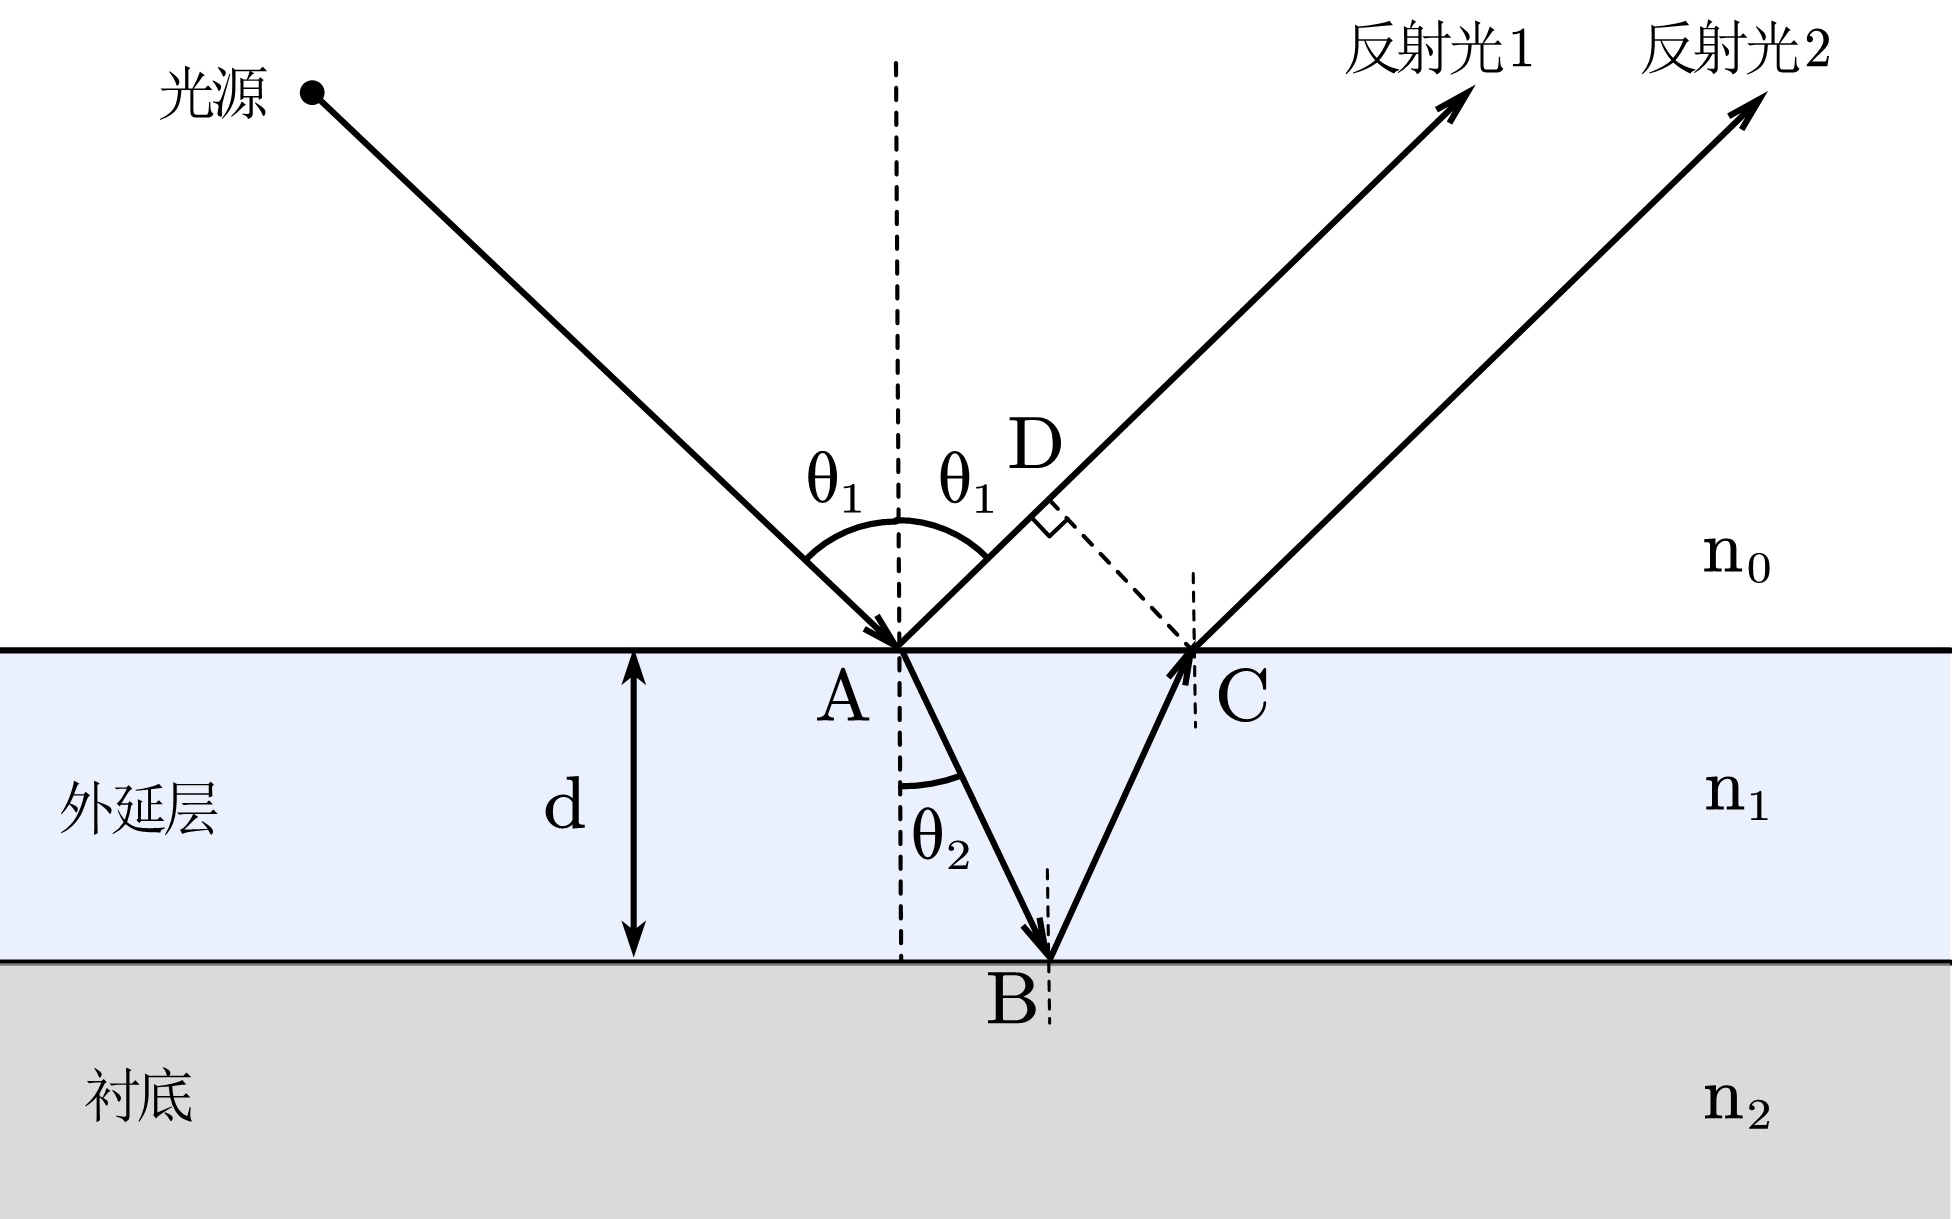
\includegraphics[width=0.6\linewidth]{双光束光路图.png}
    \caption{双光束干涉光路图}
    \label{fig:placeholder}
\end{figure}

考虑反射光1和反射光2的光程差：
\begin{equation}
    L = L_{AB} + L_{BC} - L_{AD}
\end{equation}

由几何关系可以得到：
\begin{align}
    L_{AB} + L_{BC} &= \frac{2 n_1 d}{\cos \theta_2} \\
    L_{AD} &= 2 n_0 d \tan \theta_2 \sin \theta_1
\end{align}
带入总光程差表达式，得到：
\begin{equation}
    L = 2n_1dcos\theta_2
\end{equation}

两束相干光叠加后的总光强取决于它们之间的相位差 $\delta$。该相位差由光程差和反射时可能发生的相位突变共同决定：
\begin{equation}
\delta = \frac{4\pi n_1 d \cos\theta_2}{\lambda_0} + \Phi_{\text{sub}} - \Phi_{\text{air}}
\label{dis}
\end{equation}
其中，$d$ 是外延层的厚度，$\lambda_0$ 是真空中光的波长，$n_1$ 是外延层的折射率，$\theta_2$ 是光在外延层中的折射角。$\Phi_{\text{sub}}$ 和 $\Phi_{\text{air}}$ 分别是光在外延层/衬底界面和空气/外延层界面反射时产生的相位突变。

假定入射光为非偏振光，其振幅可以分解为相互垂直的s偏振（垂直于入射面）和p偏振（平行于入射面）两个分量。设入射光的s偏振和p偏振分量振幅均为 $A_0$，则总入射光强为 $I_0 = 2A_0^2$。

两束反射光干涉后，s偏振和p偏振的总反射光强 $I_s$ 和 $I_p$ 分别为：
\begin{align}
I_s &= A_{1s}^2 + A_{2s}^2 + 2A_{1s}A_{2s}\cos(\delta_s) \\
I_p &= A_{1p}^2 + A_{2p}^2 + 2A_{1p}A_{2p}\cos(\delta_p)
\end{align}
其中，$A_{1s}, A_{1p}$ 和 $A_{2s}, A_{2p}$ 分别是光束1和光束2的s偏振和p偏振振幅。总反射光强为 $I_r = I_s + I_p$，最终的反射率 $R$ 定义为：
\begin{equation}
R = \frac{I_r}{I_0} = \frac{I_s + I_p}{2A_0^2}
\end{equation}

\subsubsection{振幅计算：菲涅尔方程的应用}
根据菲涅尔公式，可以得到反射与透射的p光和s光振幅与入射振幅关系。
\begin{figure}[htbp]
  \centering
  % 指定图片文件，png/jpg/pdf 都可以
  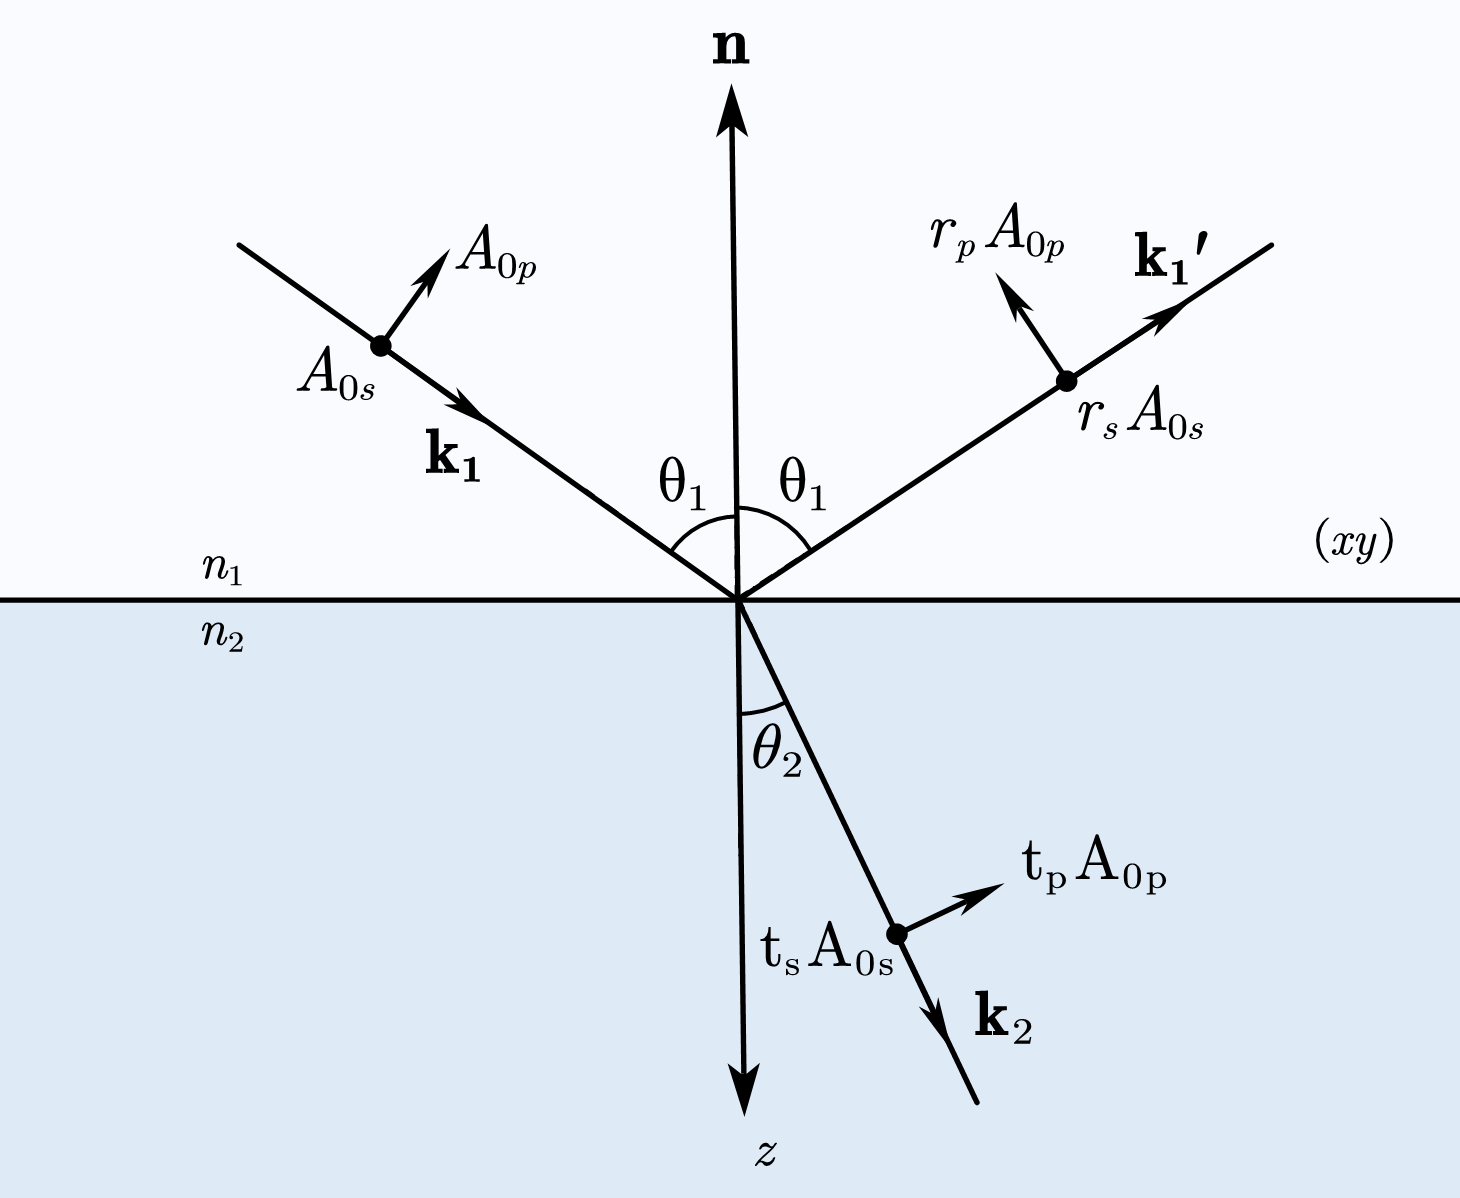
\includegraphics[width=0.6\textwidth]{菲涅尔公式演示图-有色.png}
  \caption{光在介质界面反射折射的基本物理图像}
  \label{fig:example}
\end{figure}
各反射光束和透射光束的振幅由描述电磁波在不同介质界面行为的菲涅尔方程确定。对于从介质 $i$ 入射到介质 $j$ 的情况，其振幅反射系数 ($r$) 和透射系数 ($t$) 为：
\begin{align}
r_s &= \frac{n_i \cos\theta_i - n_j \cos\theta_j}{n_i \cos\theta_i + n_j \cos\theta_j} & t_s &= \frac{2 n_i \cos\theta_i}{n_i \cos\theta_i + n_j \cos\theta_j} \\
r_p &= \frac{n_j \cos\theta_i - n_i \cos\theta_j}{n_j \cos\theta_i + n_i \cos\theta_j} & t_p &= \frac{2 n_i \cos\theta_i}{n_j \cos\theta_i + n_i \cos\theta_j}
\label{fen}
\end{align}
其中，$n_i, n_j$ 和 $\theta_i, \theta_j$ 分别是两介质的折射率和光线角度，它们通过斯涅尔定律 $n_i \sin\theta_i = n_j \sin\theta_j$ 相关联。

基于此，我们可以精确计算光束1和光束2的振幅。设空气折射率为 $n_0=1$，外延层折射率为 $n_1$，衬底折射率为 $n_2$。
\begin{itemize}
    \item \textbf{光束1 (空气/外延层界面反射):}
    \begin{align}
        A_{1s} &= r_s^{(0\to 1)} A_0 = \frac{n_0 \cos\theta_0 - n_1 \cos\theta_1}{n_0 \cos\theta_0 + n_1 \cos\theta_1} A_0 \\
        A_{1p} &= r_p^{(0\to 1)} A_0 = \frac{n_1 \cos\theta_0 - n_0 \cos\theta_1}{n_1 \cos\theta_0 + n_0 \cos\theta_1} A_0
    \end{align}
    \item \textbf{光束2 (空气$\to$外延层透射 $\to$ 衬底反射 $\to$ 外延层$\to$空气透射):}
    其振幅是多次透射和一次反射过程的乘积：
    \begin{equation}
        A_{2s} = t_s^{(0\to 1)} r_s^{(1\to 2)} t_s^{(1\to 0)} A_0 \quad \text{和} \quad A_{2p} = t_p^{(0\to 1)} r_p^{(1\to 2)} t_p^{(1\to 0)} A_0
    \end{equation}
\end{itemize}
将上述振幅表达式代入光强公式，即可得到总反射率 $R$ 作为外延层厚度 $d$、波长 $\lambda$、入射角 $\theta_0$ 以及各层折射率的函数。

\subsection{色散模型：材料光学常数的精确描述}
题目指出，外延层的折射率$n$并非一个常数。我们通过观察附件1和2的实验光谱，发现实验光谱存在“剩余射线带”，传统的塞尔迈耶方程无法描述此特质。为了精确地模拟光谱，在AI\cite{ai:gemini}的搜索功能帮助下，我们采了用因式分解形式的洛伦兹-德鲁德(Lorentz-Drude) 色散模型。该模型通过复介电函数 $\varepsilon(\omega)$ 来描述材料的光学响应，其表达式由文献\cite{oishi2006simultaneous}给出：
\begin{equation}
\varepsilon(\omega) = \varepsilon_{\infty} \left( \frac{\omega_L^2 - \omega^2 - i\gamma_L\omega}{\omega_T^2 - \omega^2 - i\gamma_T\omega} \right) - \frac{\omega_p^2}{\omega^2 + i\gamma_p\omega}
\label{eq:lorentz_drude}
\end{equation}

该模型结合了两种物理机制：第一项（洛伦兹振子项）描述了由晶格振动（声子）引起的共振吸收；第二项（德鲁德项）则描述了由掺杂引入的自由载流子的响应。

德鲁德项中的等离子体频率 $\omega_p$ 和阻尼 $\gamma_p$ 与材料的关键电学性质——载流子浓度 $N$ 和迁移率 $\mu$ 直接相关：
\begin{align}
    \omega_p^2 &= \frac{Nq^2}{\varepsilon_0 m^*} \label{eq:plasma_freq} \\
    \gamma_p &= \frac{q}{m^*\mu} \label{eq:damping_rate}
\end{align}

最终，材料复折射率$\tilde{n}(\omega) = n(\omega) + ik(\omega)$可通过以下关系式由复介电函数得到：
\begin{equation}
    \tilde{n}(\omega) = \sqrt{\varepsilon(\omega)}
\end{equation}
其中，实部 $n(\omega)$ 为我们需要的折射率，虚部 $k(\omega)$ 为消光系数。由于折射率是复数，菲涅尔系数和相位差的计算都将在复数域中进行，这自然地包含了吸收和相位突变效应。

\section{问题二的模型建立与求解}
问题二中，我们使用了问题一的双光束干涉模型以及洛伦兹-德鲁德色散模型，并根据文献确定了模型的部分基本参数，以附件1和2的实验数据为基准，对模型中未知的七个关键参数进行全局优化拟合，从而解出一组最优参数，最终确定外延层的厚度。
\subsection{决策变量的选取}
外延层和衬底的复介电函数 $\varepsilon(\sigma)$ 由公式（\ref{eq:lorentz_drude}）描述。

由题意，外延层和衬底为同种材质，但由于掺杂载流子浓度的不同而有不同的折射率。因此外延层和衬底的介电系数共享相同的晶格参数($\varepsilon_{\infty}, \omega_L, \omega_T, \gamma_L, \gamma_T$)。而载流子浓度的不同影响到材料的自由载流子响应项和迁移率，反映在外延层和衬底有各自的德鲁德参数($\omega_{p1}, \gamma_{p1}$ 和 $\omega_{p2}, \gamma_{p2}$)。
    
因此，求解本问的决策变量包含：
\begin{equation}
    \{d, \gamma_L, \gamma_T, \omega_{p1}, \gamma_{p1}, \omega_{p2}, \gamma_{p2}\}
\end{equation}



% \subsection{模型选择与策略演进}
% 在正式确定算法之前，我们评估了较为简化的干涉条纹计数法。该方法通过识别光谱中干涉条纹极值点的位置来估算光学厚度。我们选取光谱中干涉条纹清晰且本底相对平坦的高波数区域（设定为 > \SI{1500}{cm^{-1}}）进行分析。然而，此方法在处理附件1和附件2的数据时暴露了其局限性：对于附件1（\ang{10}），计算出的厚度为 $d_1 = 22.59 \pm 0.08 \, \mu\text{m}$；而对于附件2（\ang{15}），结果为 $d_2 = 7.73 \pm 0.10 \, \mu\text{m}$。对于同一物理样品，这两组结果之间存在着巨大的、不符合物理现实的差异。

% 我们分析认为，这种差异的根源在于衬底的重掺杂特性。重掺杂使得衬底呈现出类金属的光学特性，导致光在“外延层-衬底”界面反射时发生了复杂的、随频率变化的相位突变。简单的干涉条纹计数法假设相位变化为0或$\pi$，无法描述这种复杂的相位行为，因此导致了错误的厚度计算结果。

% 综合以上考量，我们最终确定采用问题一中建立的\textbf{双光束干涉模型}与\textbf{洛伦兹-德鲁德色散模型}相结合的策略。该组合能够从物理层面精确描述介电常数随频率的变化以及由此引发的复杂相位关系，对实验数据的拟合表现出更好的鲁棒性和物理真实性。

\subsection{求解模型的数学框架}
我们的任务是解决一个逆问题，即通过拟合实验光谱 $R_{\text{exp}}(\sigma)$ 来反向拟合出样品未知的物理参数。具体来说，我们设定了7个待拟合物理参数，需要通过固定物理参数计算出理论反射光谱，和实验光谱数据进行残差分析来计算出残差最小时对应的参数组合。

首先，我们假设样品为4H-SiC材料，参考文献中的物理参数，从而简化模型的计算。经过AI\cite{ai:gemini}搜索，该材料的本征光学参数可以依据文献\cite{oishi2006simultaneous}设定，具体如表（\ref{tab:sic_params}）所示。

\begin{table}[h!]
\centering
\caption{4H-SiC材料固定的本征光学参数}
\label{tab:sic_params}
\begin{tabular}{@{}llll@{}}
\toprule
参数 & 符号 & 数值 & 单位 \\ \midrule
高频介电常数 & $\varepsilon_{\infty}$ & 6.56 & (无量纲) \\
纵向光学声子频率 & $\omega_L$ & 970.0 & \si{cm^{-1}} \\
横向光学声子频率 & $\omega_T$ & 798.0 & \si{cm^{-1}} \\ \bottomrule
\end{tabular}
\end{table}
我们的算法模型目标是求解出最优的一组参数向量$\mathbf{p}$，它们与介电函数紧密相关：
\begin{equation}
    \mathbf{p} = \{d, \gamma_L, \gamma_T, \omega_{p1}, \gamma_{p1}, \omega_{p2}, \gamma_{p2}\}
\end{equation}

这些参数通过以下物理链条决定最终的反射率：

\begin{enumerate}
    \item \textbf{光学模型决定介电函数：} 外延层和衬底的复介电函数 $\varepsilon(\sigma)$ 由公式（\ref{eq:lorentz_drude}）描述。
    其中，外延层和衬底共享相同的晶格参数($\varepsilon_{\infty}, \omega_L, \omega_T, \gamma_L, \gamma_T$)，但具有不同的德鲁德项参数($\omega_{p1}, \gamma_{p1}$ 和 $\omega_{p2}, \gamma_{p2}$)。

    \item \textbf{介电函数决定光学常数与界面行为：} 复折射率 $\tilde{n}(\sigma) = \sqrt{\varepsilon(\sigma)}$ 决定了光在空气/外延层和外延层/衬底界面上的反射与透射行为，这些行为由菲涅尔方程精确描述。

    \item \textbf{厚度决定干涉效应：} 外延层的厚度 $d$ 决定了两束反射光之间的相位差 $\delta$，关系见公式（\ref{dis}）。最终的非偏振光反射率 $R$ 由此确定。
\end{enumerate}

我们需要寻找最优的$\mathbf{p}_{\text{opt}}$，使得理论反射率 $R_{\text{theory}}(\sigma; \mathbf{p})$ 与实验数据 $R_{\text{exp}}(\sigma)$ 的差异最小。问题二求解的算法流程图如图（\ref{fig:process}）。

\begin{figure}[H]
    \centering
    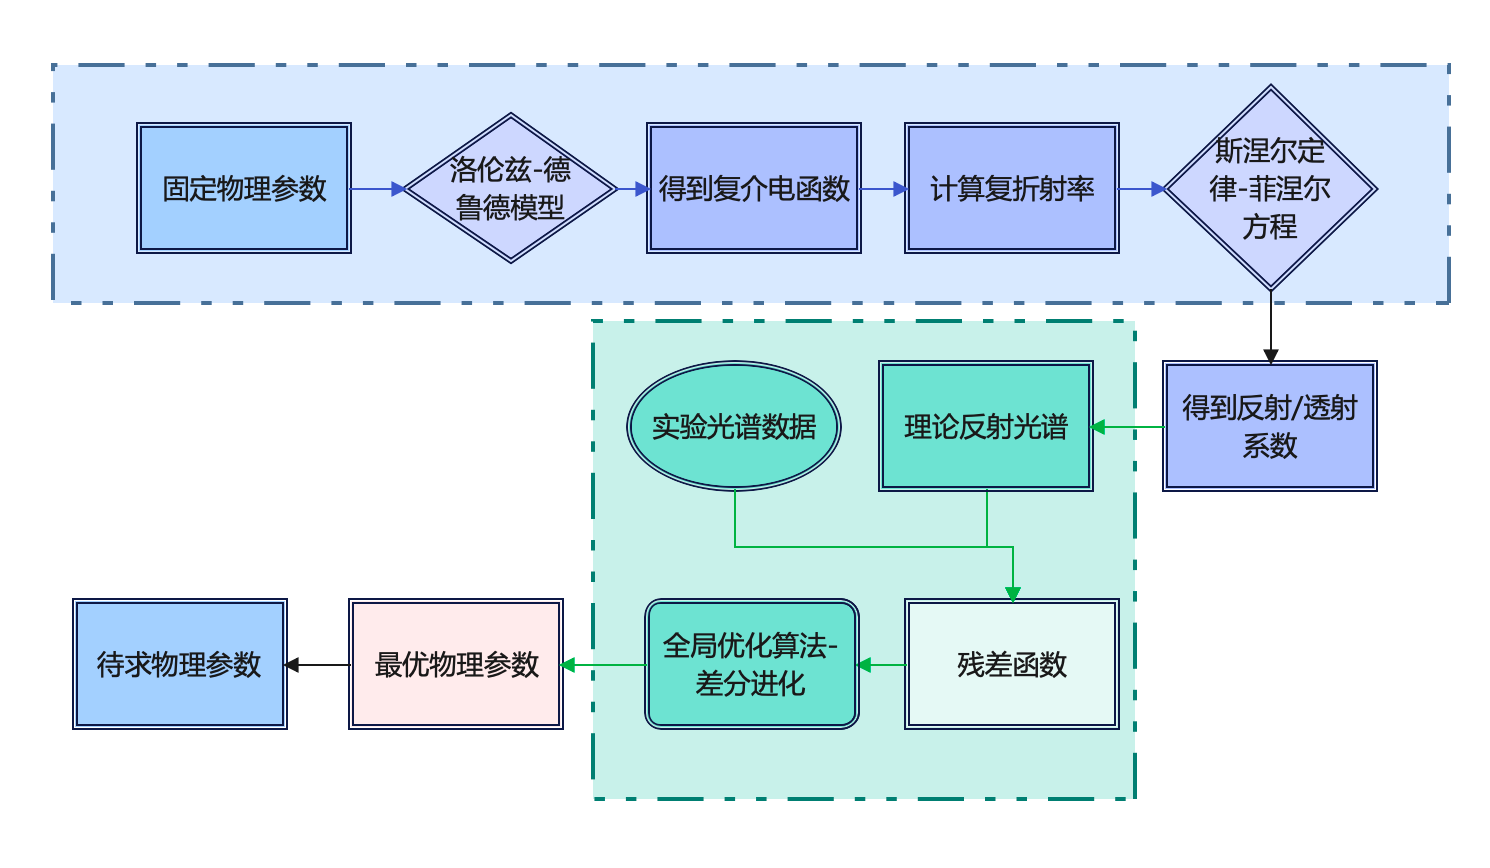
\includegraphics[width=0.75\textwidth]{流程.png} 
    \caption{问题二求解算法流程图}
    \label{fig:process}
\end{figure}


\subsection{算法设计}

% \subsubsection{固定参数}
% 为了确保模型的物理真实性并降低优化问题的复杂度，我们假设样品为4H-SiC材料。其本征的晶格振动参数依据文献\cite{oishi2006simultaneous}设定为固定值，具体如表 \ref{tab:sic_params} 所示。

% \begin{table}[h!]
% \centering
% \caption{4H-SiC材料固定的本征光学参数}
% \label{tab:sic_params}
% \begin{tabular}{@{}llll@{}}
% \toprule
% 参数 & 符号 & 数值 & 单位 \\ \midrule
% 高频介电常数 & $\varepsilon_{\infty}$ & 6.56 & (无量纲) \\
% 纵向光学声子频率 & $\omega_L$ & 970.0 & \si{cm^{-1}} \\
% 横向光学声子频率 & $\omega_T$ & 798.0 & \si{cm^{-1}} \\ \bottomrule
% \end{tabular}
% \end{table}

\subsubsection{优化策略与目标函数}
经过和AI\cite{ai:claude}的讨论，我们决定采用全局同步拟合算法，即寻找一组唯一的物理参数向量 $\mathbf{p}$，使其能够同时最优地解释附件1和附件2两个独立的实验数据，所以我们设定目标函数为两个数据集均方误差（MSE）的总和：
\begin{equation}
    \chi^2_{\text{total}}(\mathbf{p}) = \text{MSE}(\mathbf{p}, \text{\ang{10}}) + \text{MSE}(\mathbf{p}, \text{\ang{15}})
\end{equation}

此策略采用了一组唯一参数来同时约束两个不同角度的光谱数据，极大地降低了多参数逆问题中普遍存在的解不唯一风险，保证了了核心厚度参数$d$的鲁棒性。
\subsubsection{优化执行步骤}
我们执行两步优化流程，以确保能够找到全局最优解，避免陷入局部极值。
\begin{enumerate}
    \item \textbf{第一步：全局搜索。} 我们使用\textbf{差分进化算法（Differential Evolution）}，在预设的参数边界内进行并行搜索。
    \item \textbf{第二步：局部优化。} 在全局搜索找到一个接近最优解的区域后，我们以差分进化算法的输出作为初始值，采用\textbf{L-BFGS-B算法}进行精细的局部优化，搜索出更加精确的结果。
\end{enumerate}



\subsection{求解过程与结果分析}
\subsubsection{数据处理与算法参数设定}
首先，我们注意到附件中的第一行数据显示反射率为0，不符合物理事实，因此予以剔除，从第二个数据点开始进行拟合。
其次，我们使用AI\cite{ai:deepseek}生成了基本的优化算法，并且自行调整参数，对于第一步的\textbf{全局优化阶段（差分进化）}，我们设定种群大小为40，最大迭代次数为1000次；同时固定随机种子为42以保证结果的可复现性。在随后的\textbf{局部优化阶段（L-BFGS-B）}，我们设定最大迭代次数为500次，并将收敛容差（\texttt{ftol}, \texttt{gtol}）设为严格的$1 \times 10^{-12}$。

\subsubsection{全光谱范围全局同步拟合}
我们将附件1和附件2提供的完整光谱数据代入上述求解算法，进行全局同步拟合。最终得到的唯一参数组$p$如表（\ref{tab:full_range_fit}）所示。

\begin{table}[h!]
\centering
\caption{全光谱范围（\SIrange{400}{4000}{cm^{-1}}）全局同步拟合参数}
\label{tab:full_range_fit}
\begin{tabular}{@{}lll@{}}
\toprule
参数 & 符号 & 拟合值 \\ \midrule
\textbf{外延层厚度} & $d$ & \textbf{\SI{7.413}{\micro\meter}} \\
声子阻尼 (纵向) & $\gamma_L$ & \SI{0.100}{cm^{-1}} \\
声子阻尼 (横向) & $\gamma_T$ & \SI{1.096}{cm^{-1}} \\
外延层等离子体频率 & $\omega_{p1}$ & \SI{457.42}{cm^{-1}} \\
外延层等离子体阻尼 & $\gamma_{p1}$ & \SI{1294.51}{cm^{-1}} \\
衬底等离子体频率 & $\omega_{p2}$ & \SI{1120.07}{cm^{-1}} \\
衬底等离子体阻尼 & $\gamma_{p2}$ & \SI{648.05}{cm^{-1}} \\ \bottomrule
\end{tabular}
\end{table}

相应的拟合曲线与实验数据对比如图（\ref{fig:full_range_plot1}）和（\ref{fig:full_range_plot2}）所示。从图中可以看出，附件1和附件2的决定系数（R²）分别高达\textbf{0.9967和0.9948}，证明了模型的高度准确性。
% \begin{figure}[h!]
% \centering
% \begin{minipage}{0.5\textwidth}
%     \centering
%     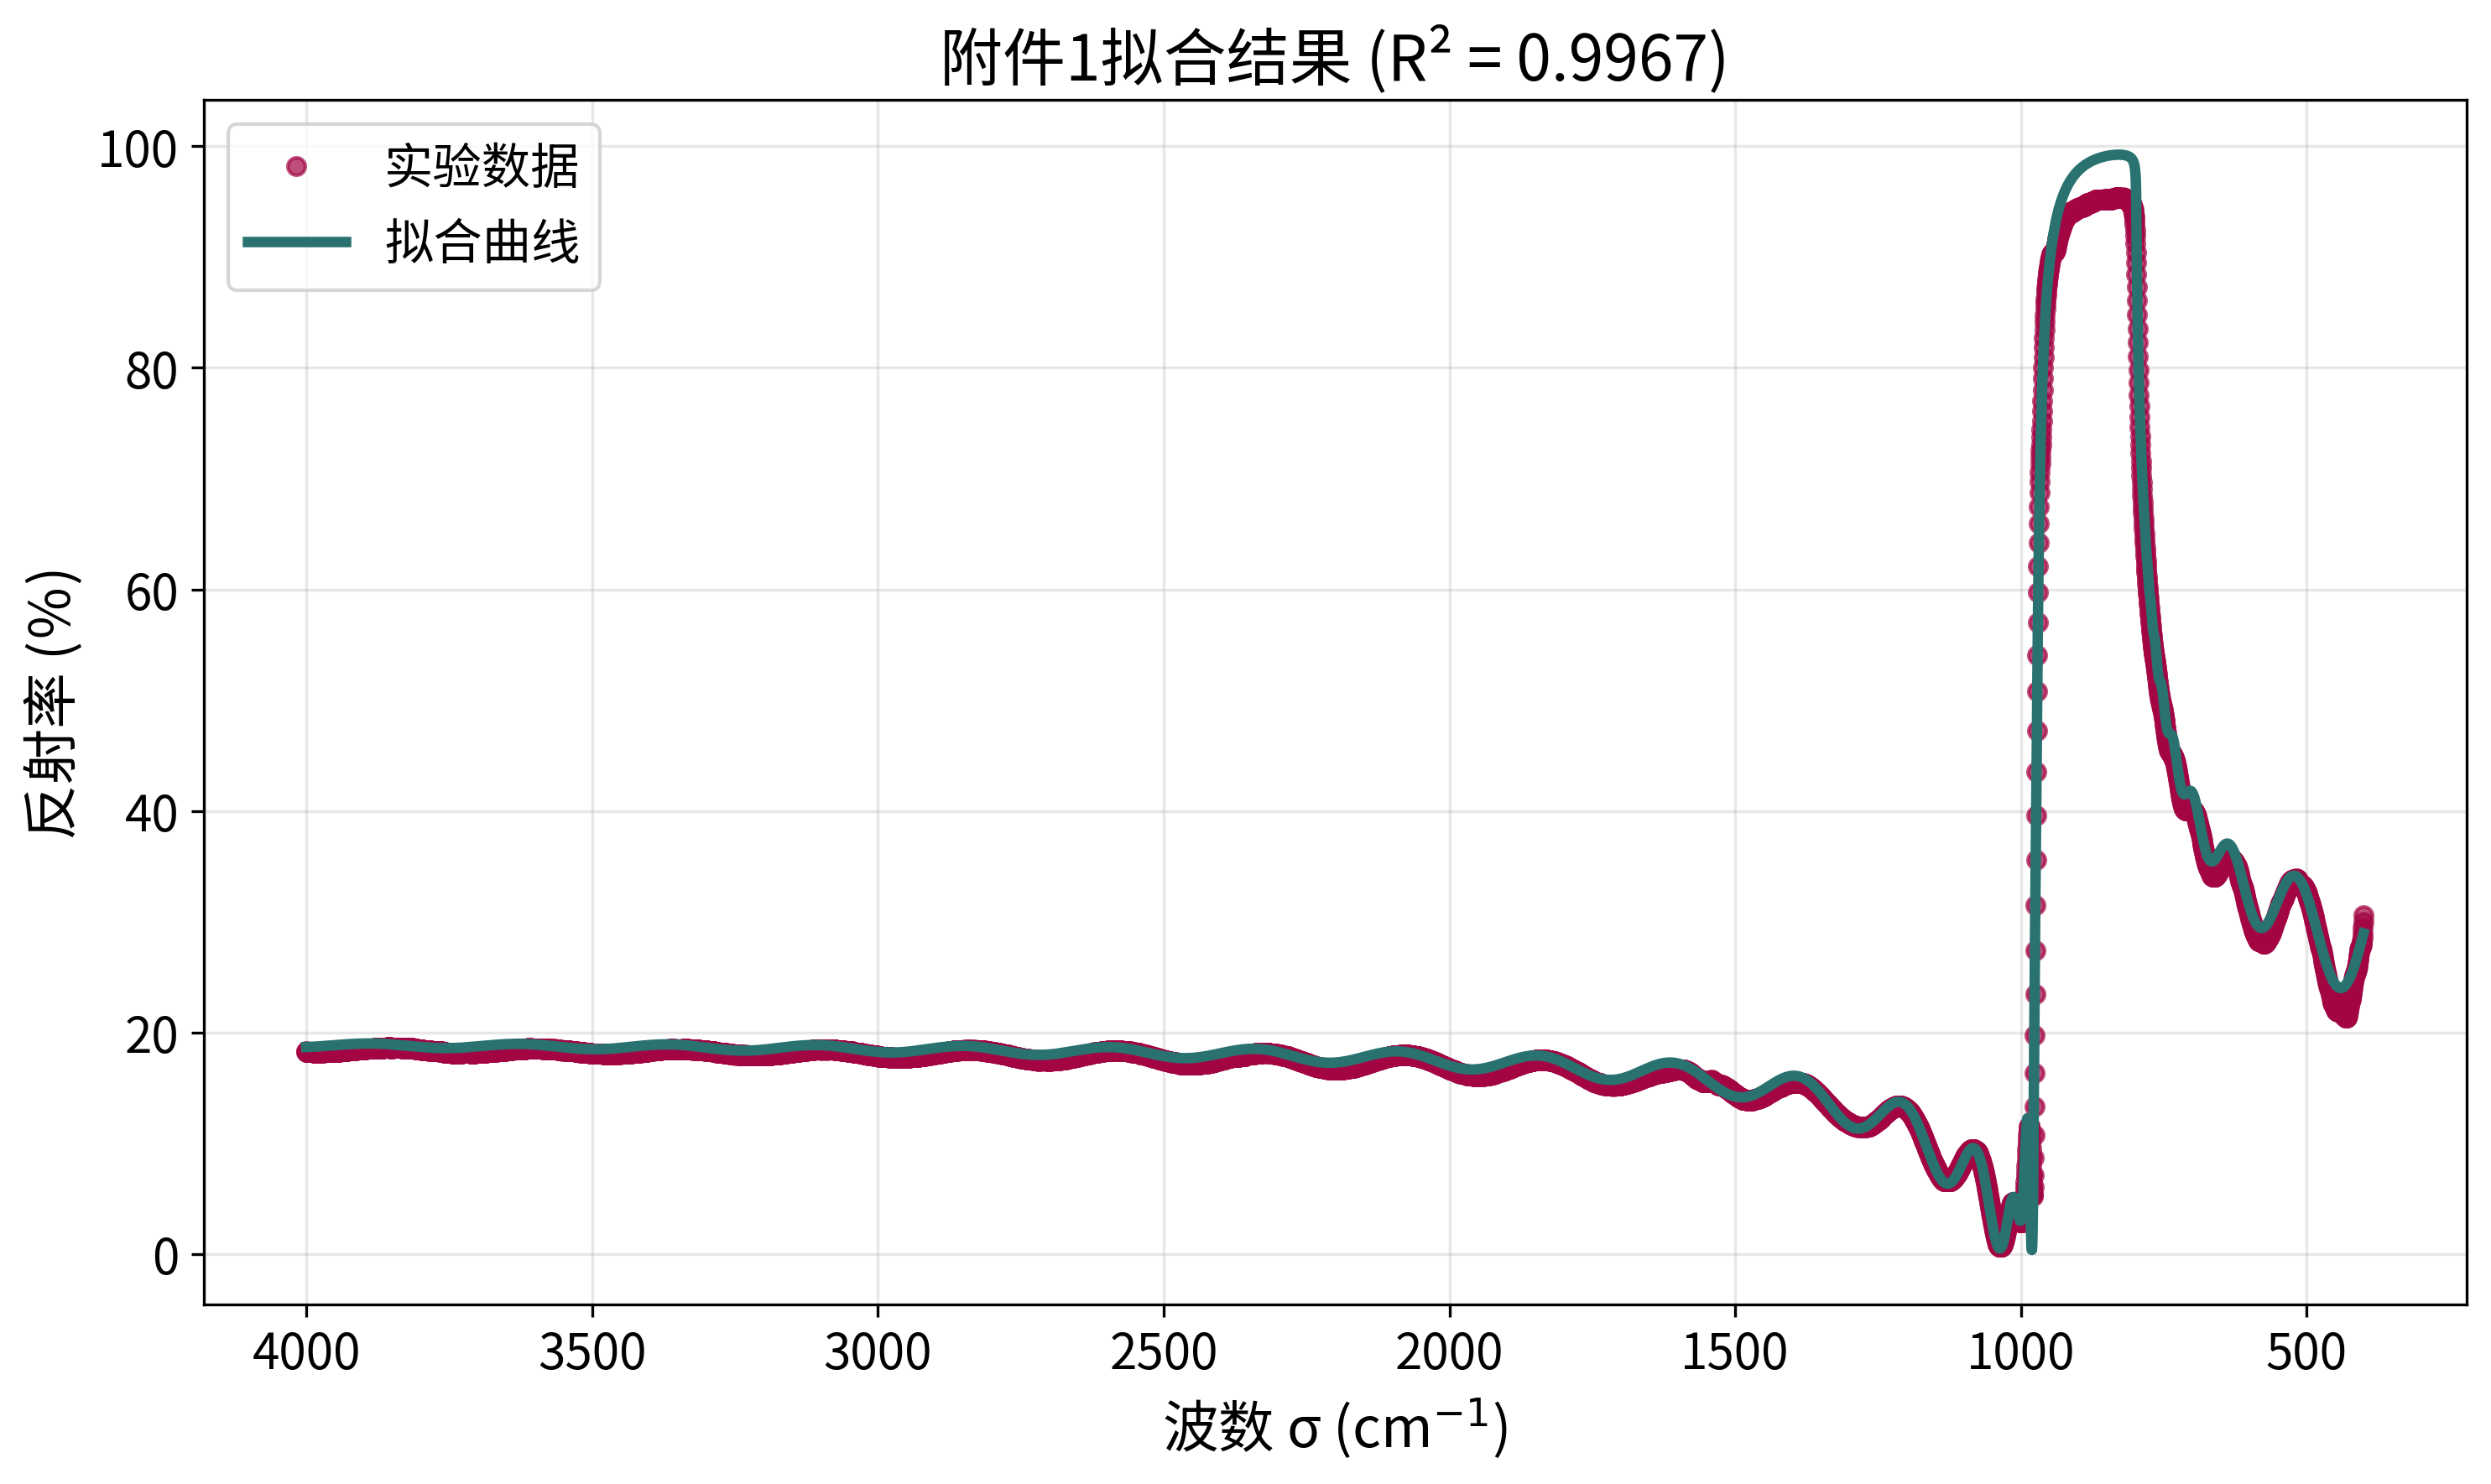
\includegraphics[width=\textwidth]{附件1拟合.png}
%     \caption{附件1全光谱范围的全局同步拟合结果（R²=0.9967）。}
%     \label{fig:1}
% \end{minipage}
% \hfill
% \begin{minipage}{0.5\textwidth}
%     \centering
%     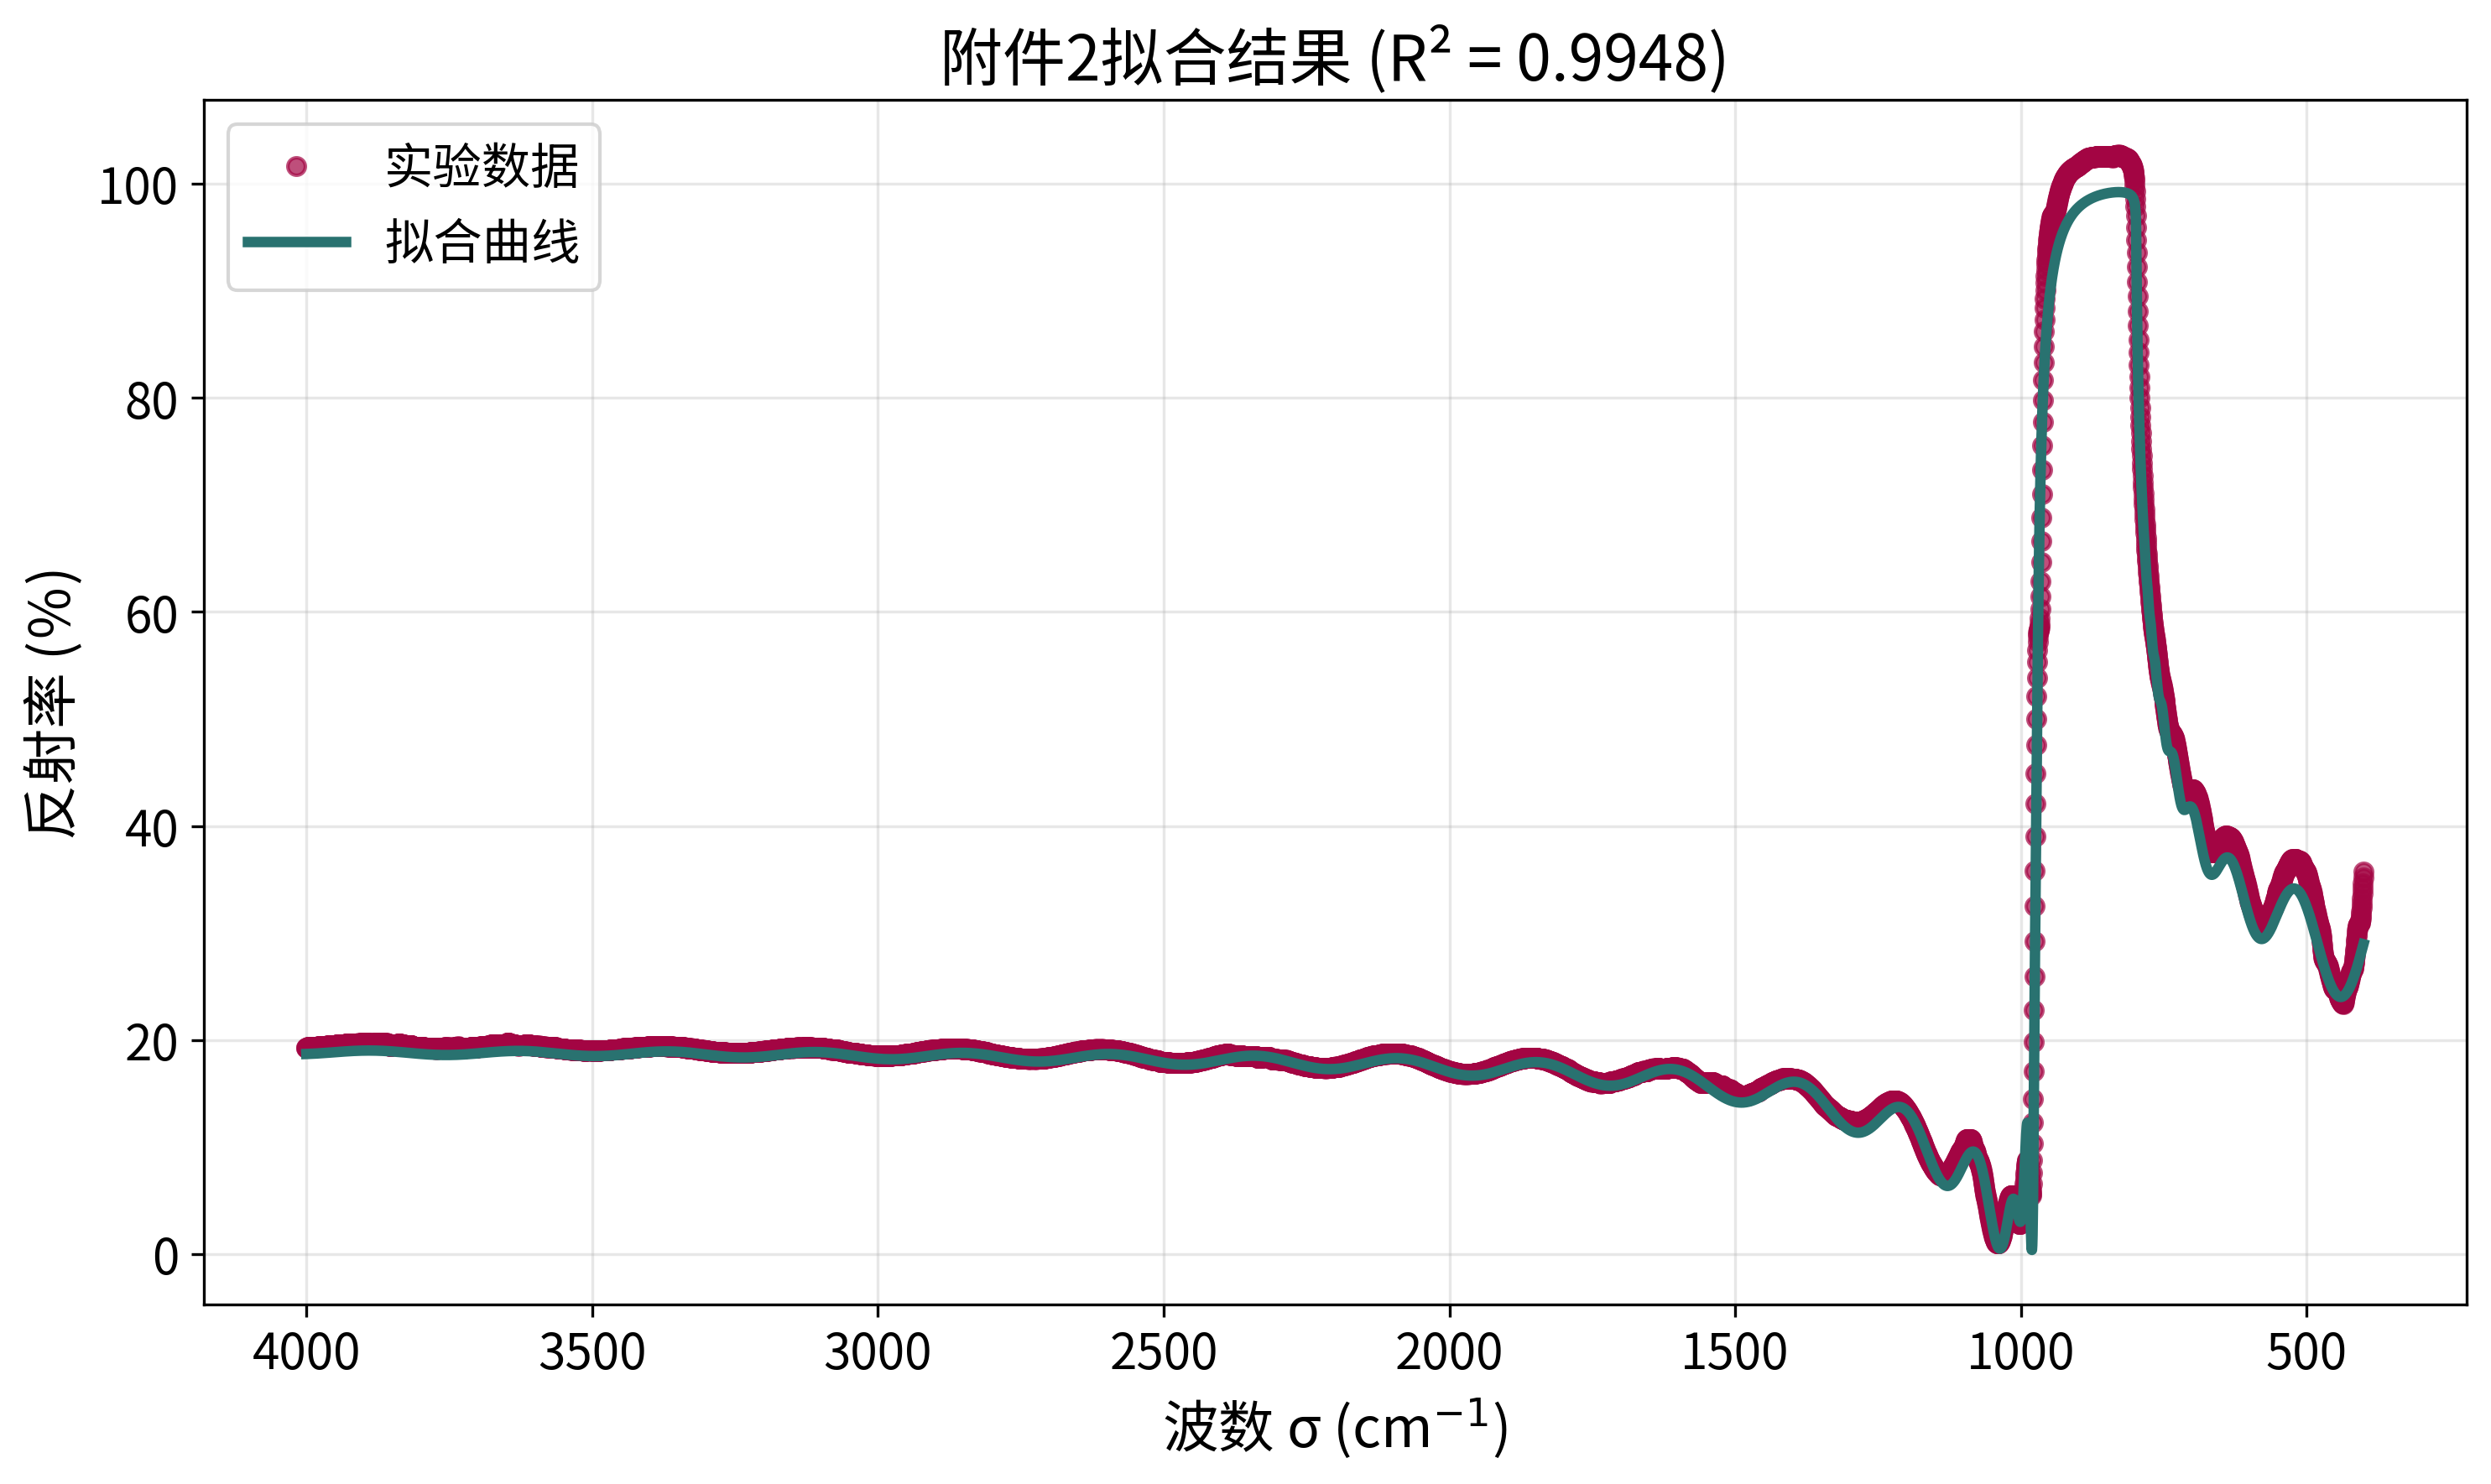
\includegraphics[width=\textwidth]{附件2拟合.png}
%     \caption{附件2全光谱范围的全局同步拟合结果（R²=0.9948）。}
%     \label{fig:2}
% \end{minipage}
% \end{figure}

\begin{figure}[h!]
    \centering
    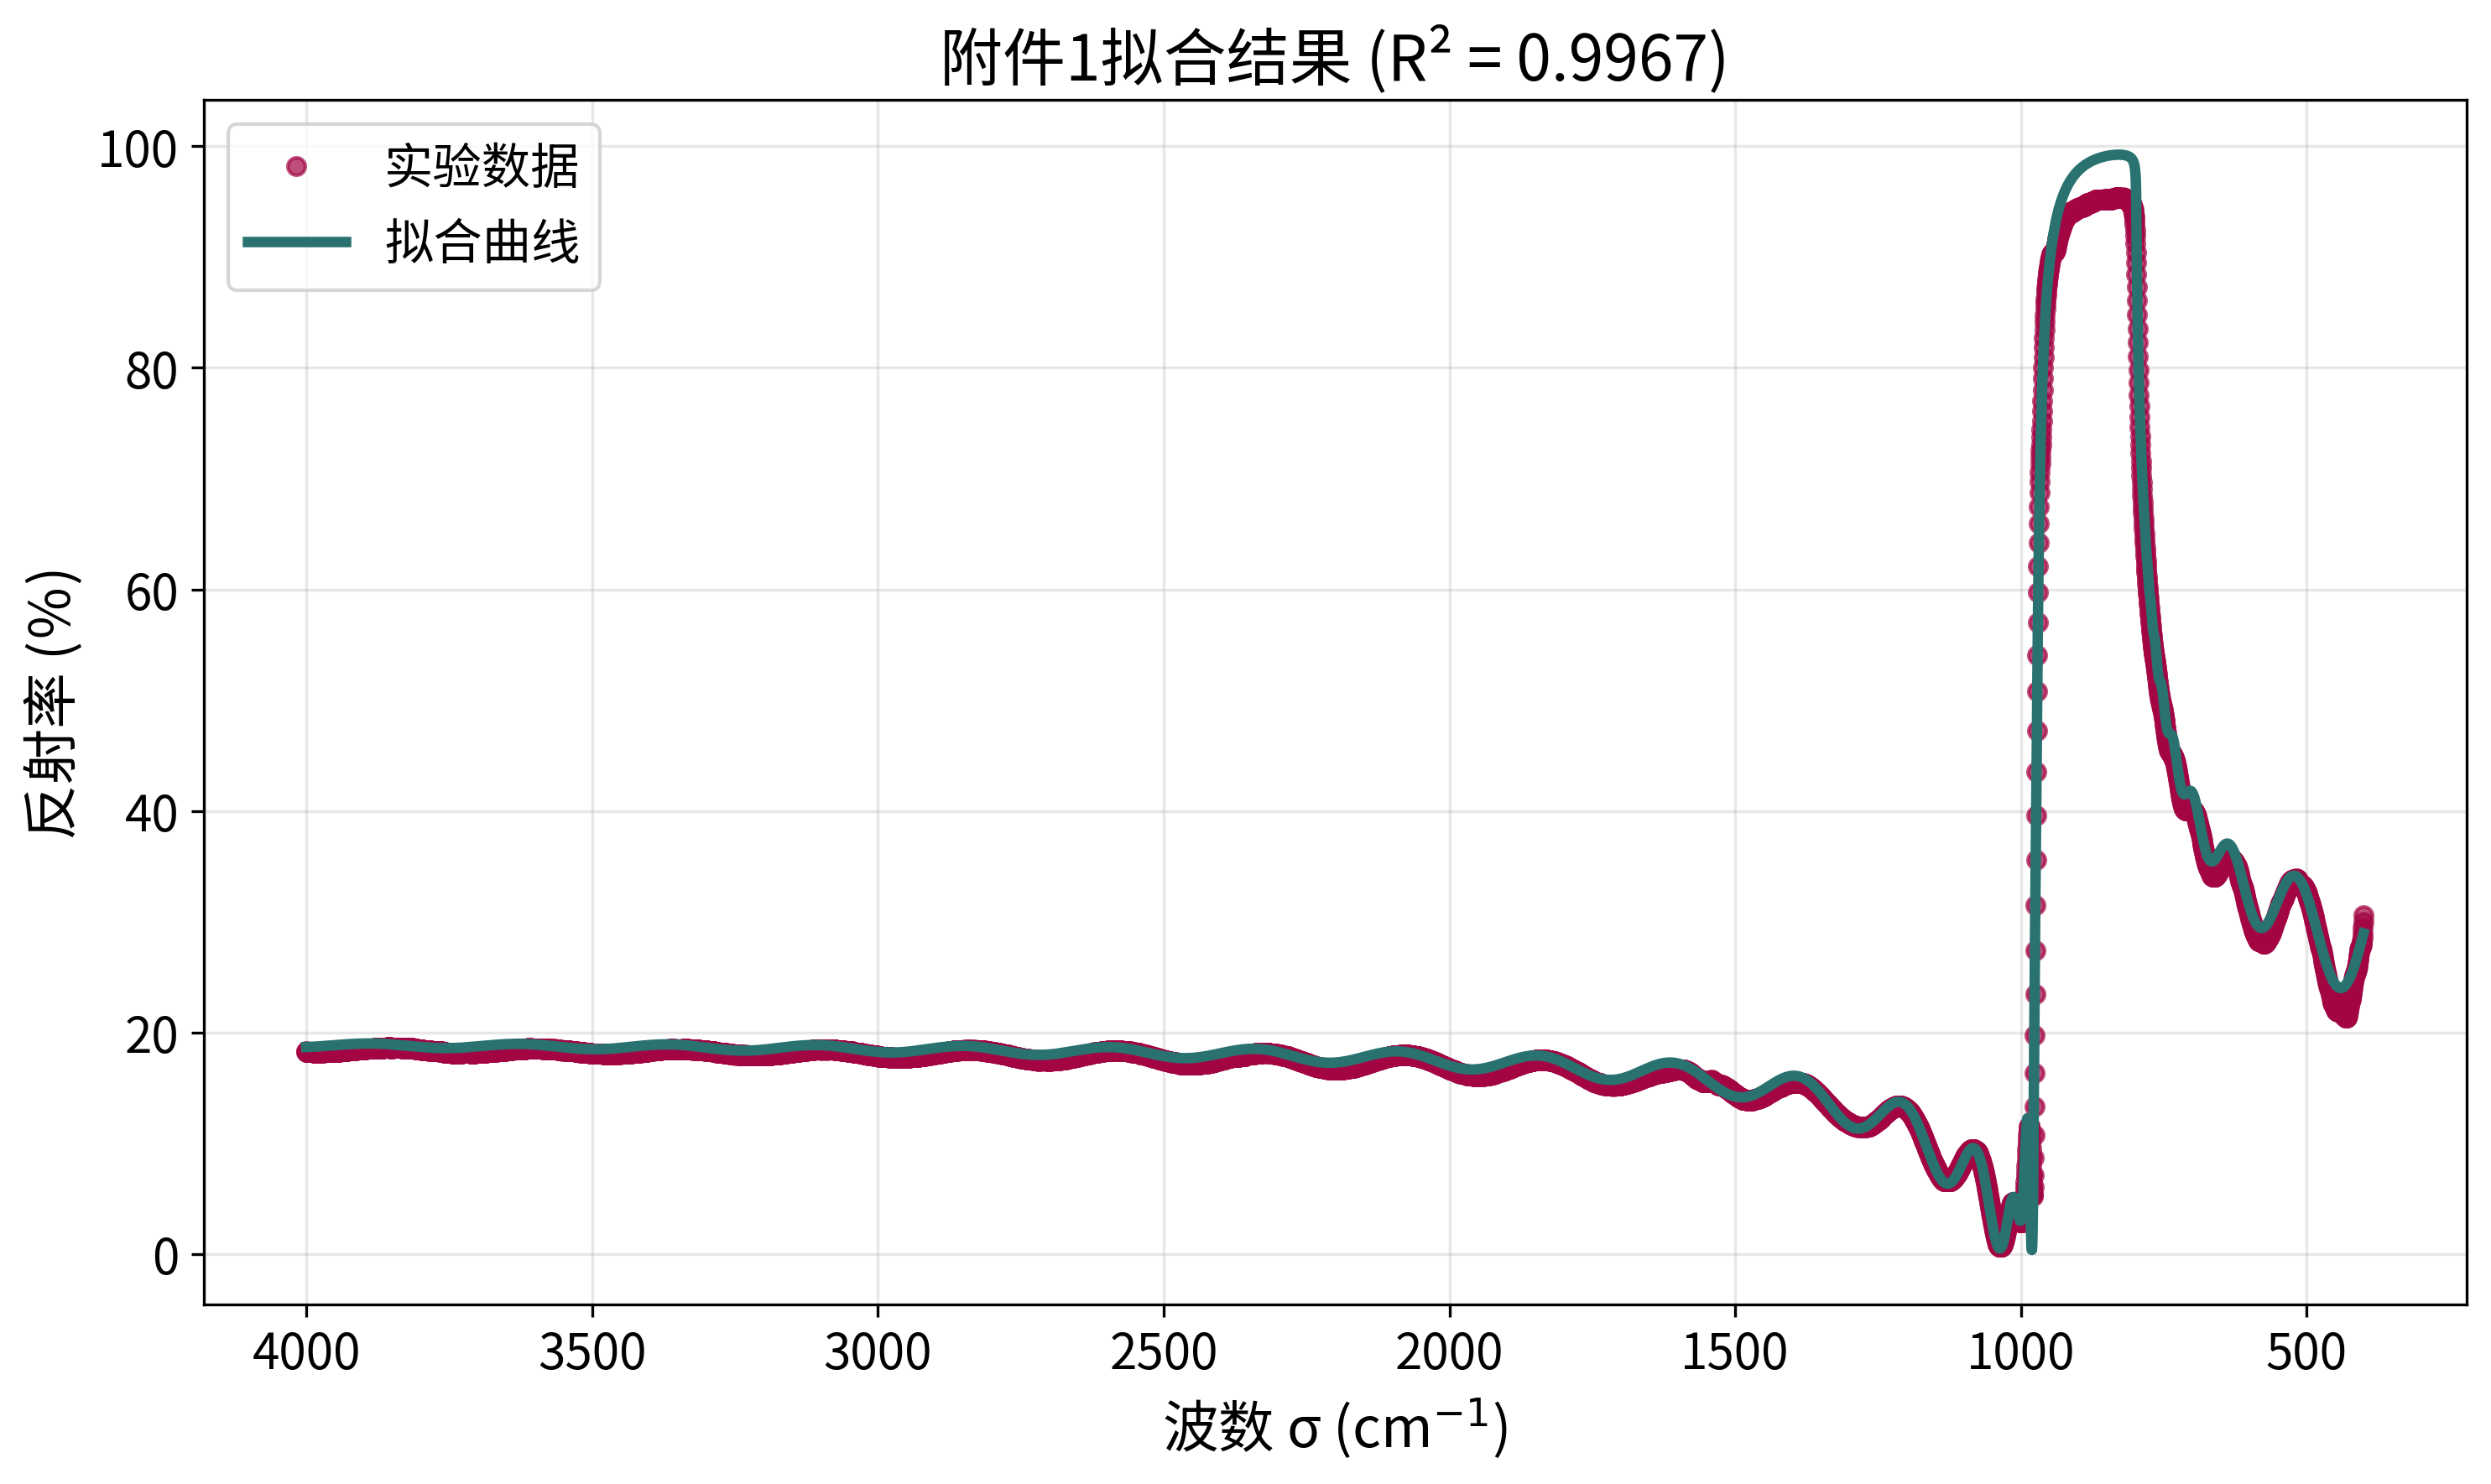
\includegraphics[width=0.7\textwidth]{附件1拟合.png} 
    \caption{附件1全光谱范围的全局同步拟合结果（R²=0.9967）。}
    \label{fig:full_range_plot1}
\end{figure}
\begin{figure}[h!]
    \centering
    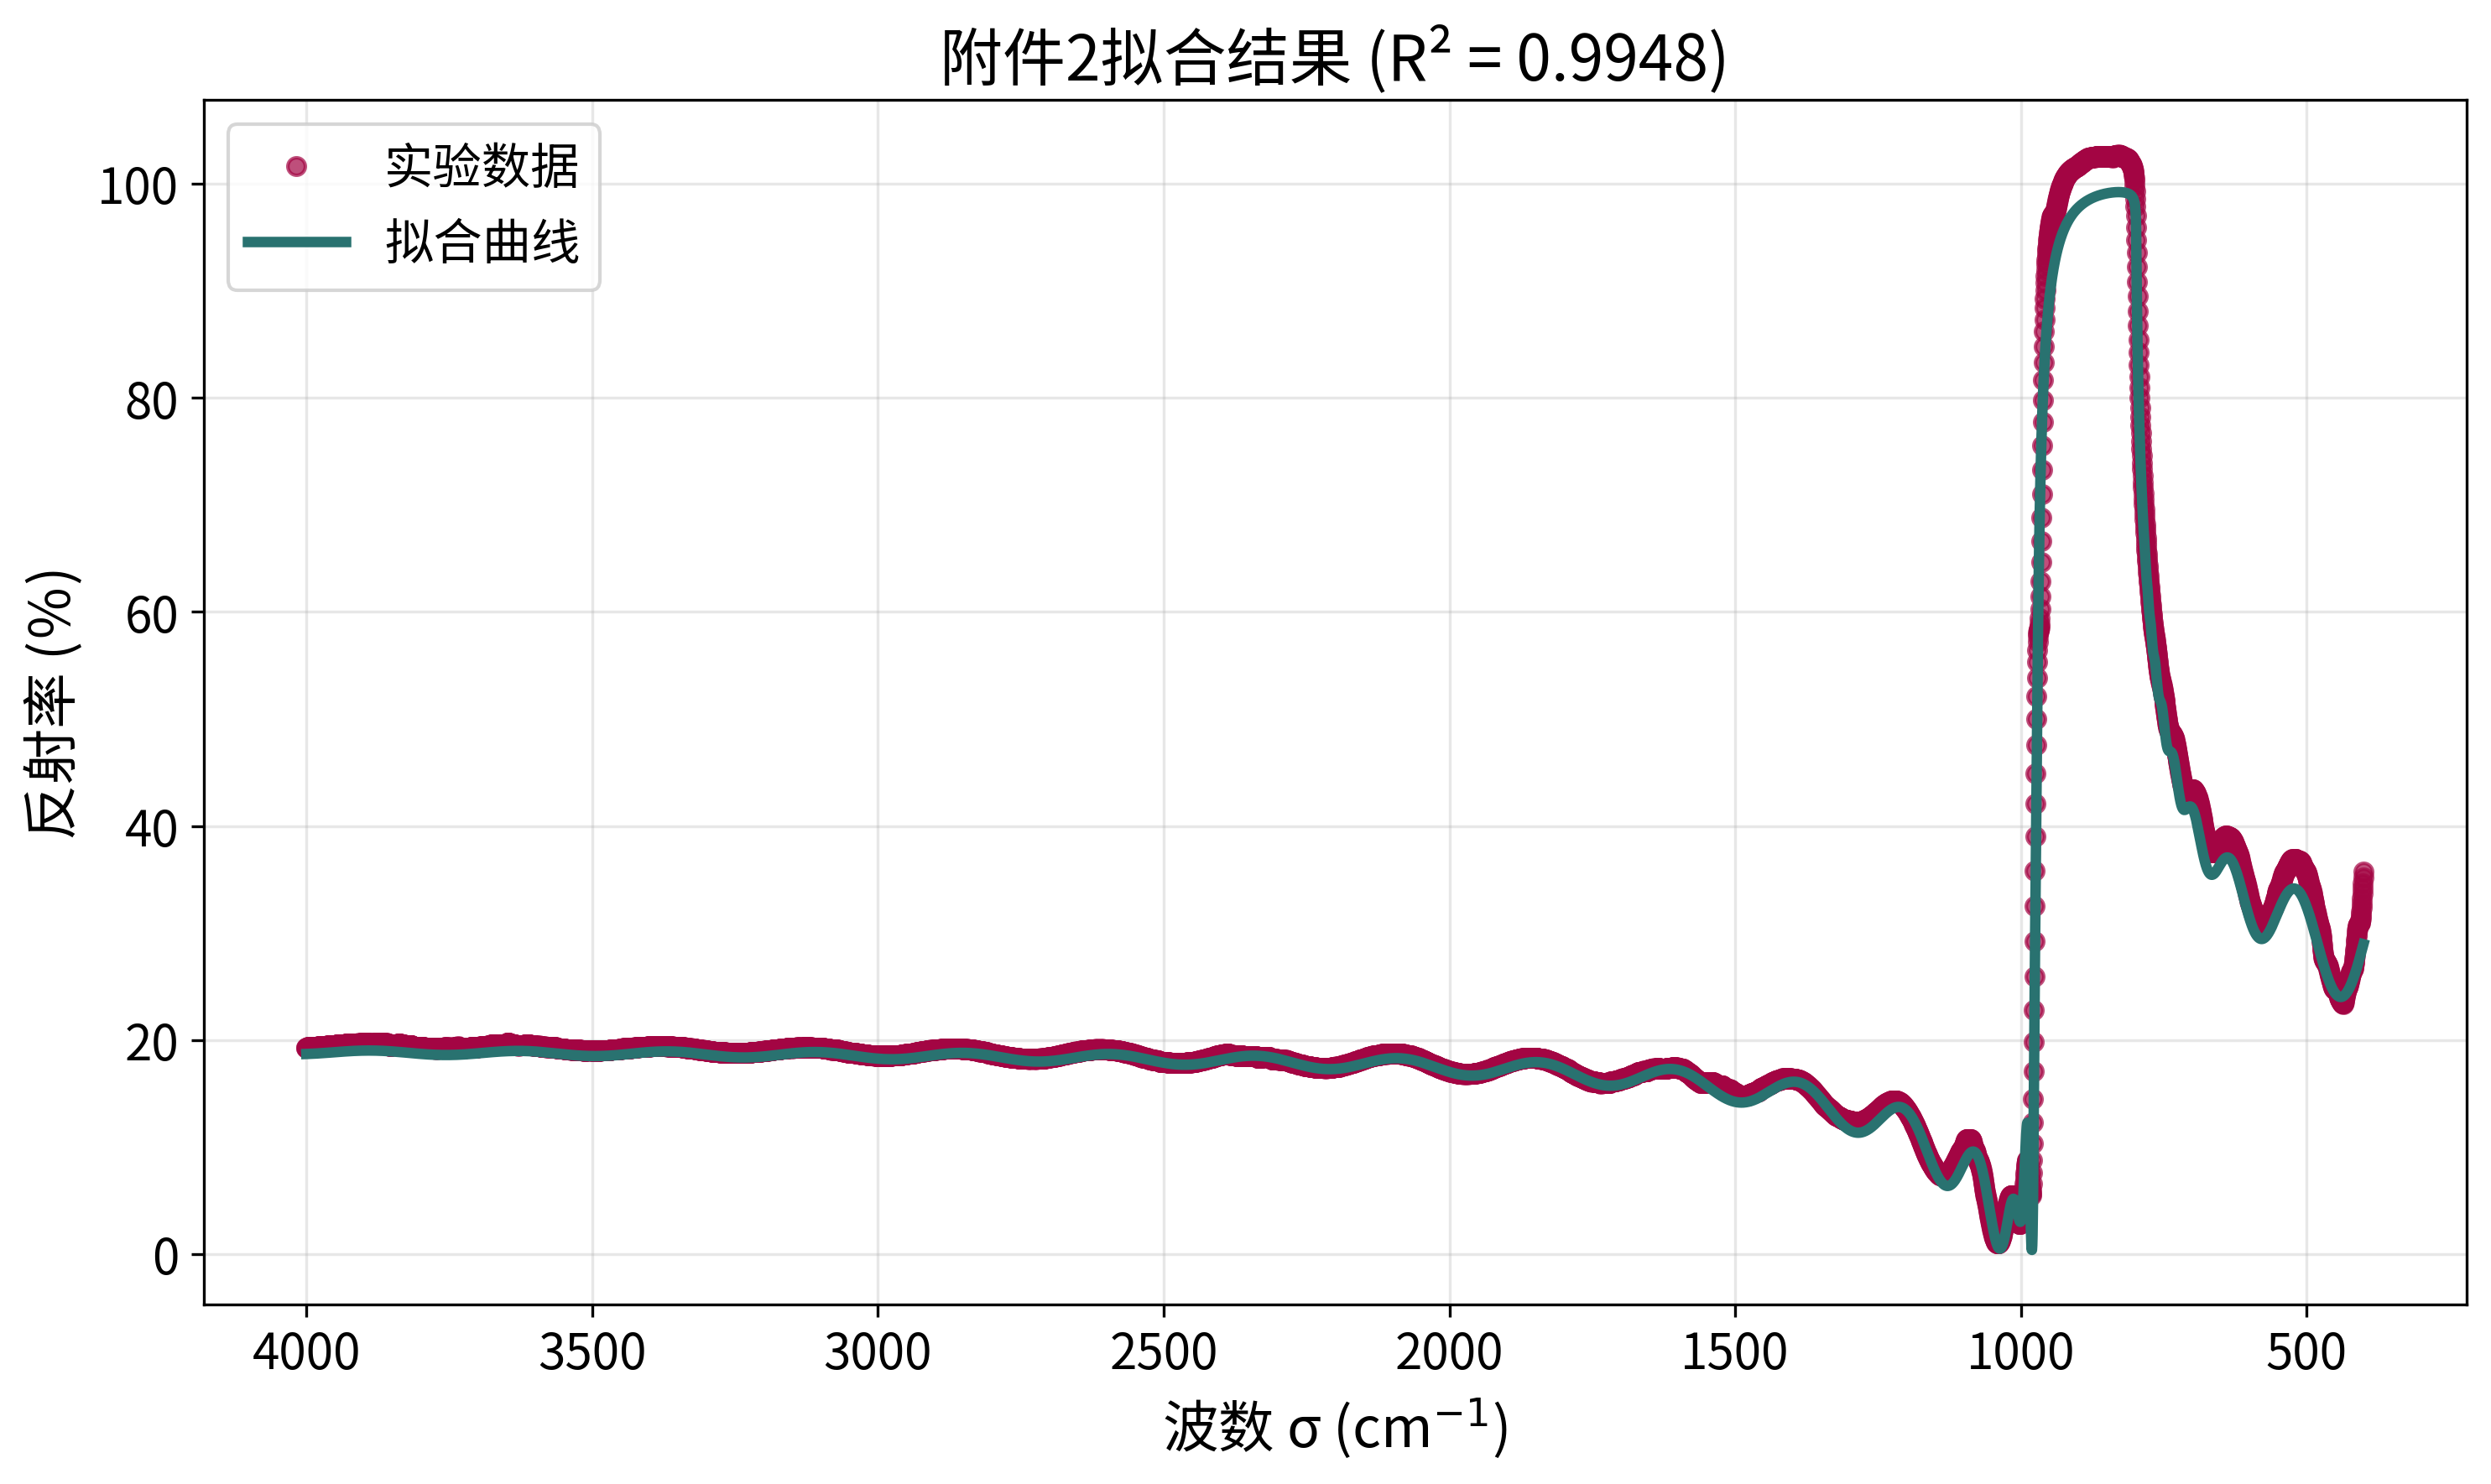
\includegraphics[width=0.7\textwidth]{附件2拟合.png} 
    \caption{附件2全光谱范围的全局同步拟合结果（R²=0.9948）。}
    \label{fig:full_range_plot2}
\end{figure}
% \begin{figure}[htbp]
%   \centering % 将整个图形块居中

%   % --- 第一个子图 (左图) ---
%   \begin{subfigure}[b]{0.49\textwidth}
%     \centering
%     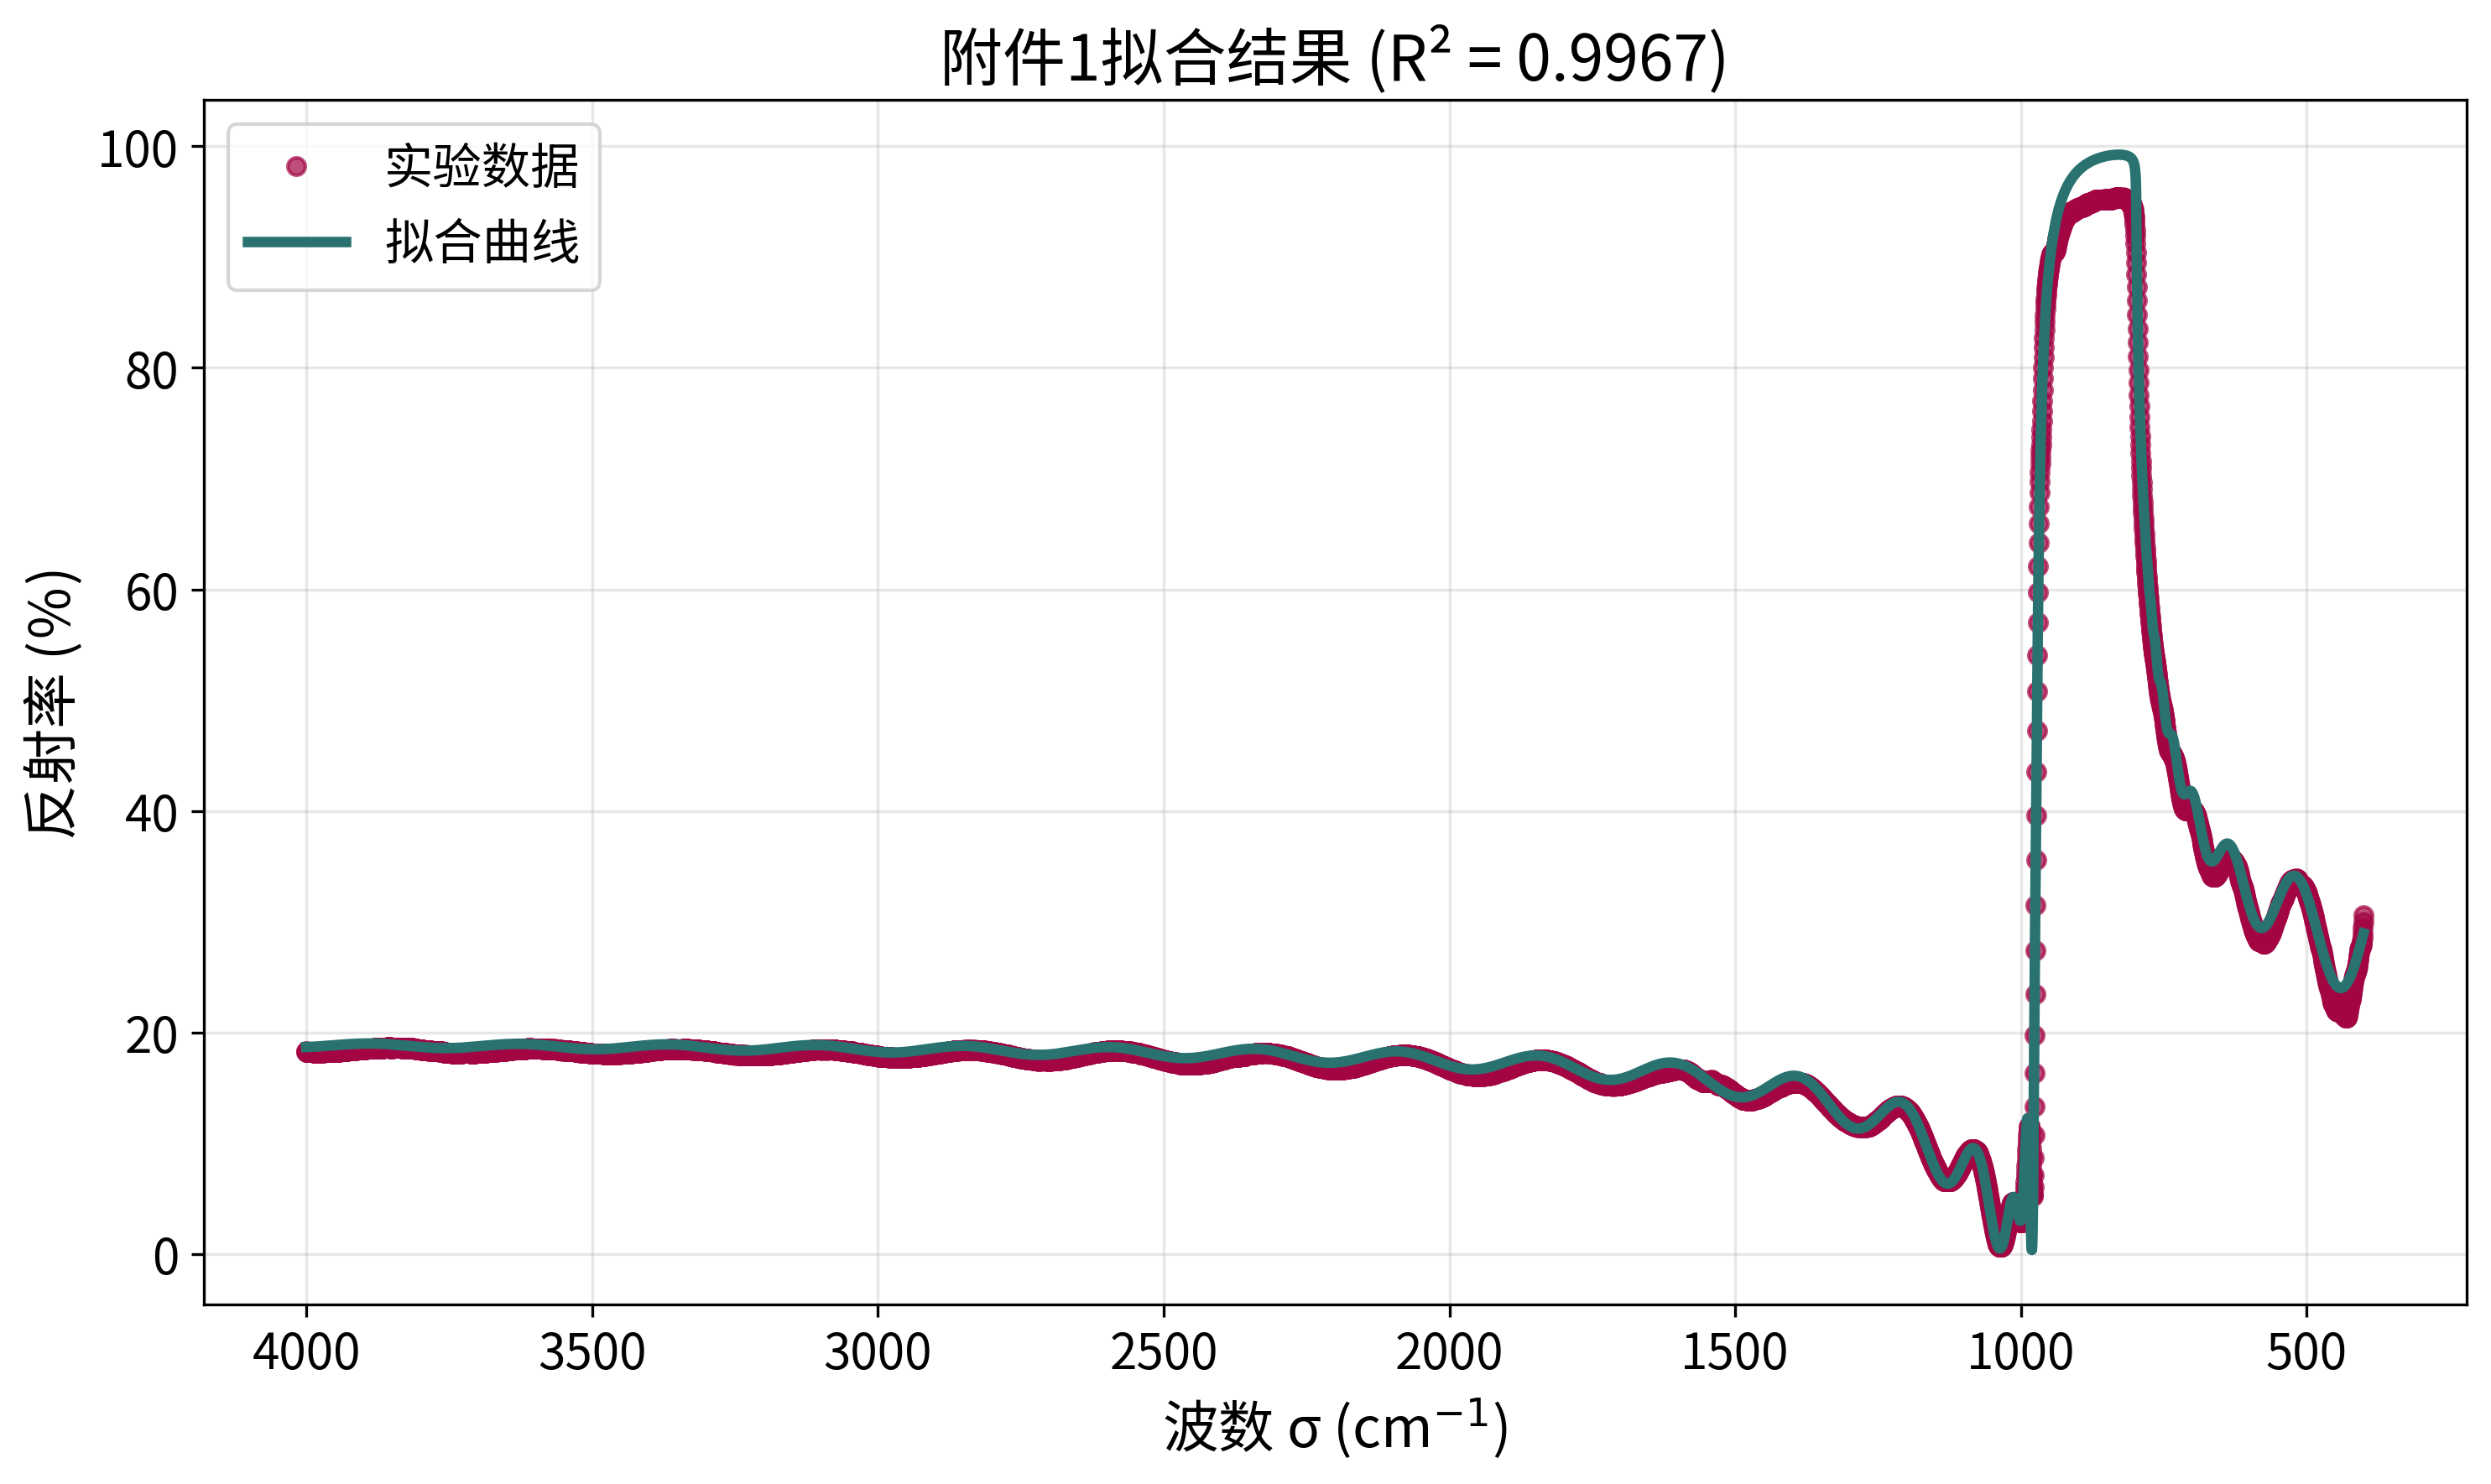
\includegraphics[width=\textwidth]{附件1拟合.png}
%     \caption{附件1全光谱范围的全局同步拟合结果（R²=0.9967）}
%     \label{fig:full_range_plot1}
%   \end{subfigure}
%   \hfill % 在两个子图之间添加一个弹性的水平间距
%   % --- 第二个子图 (右图) ---
%   \begin{subfigure}[b]{0.49\textwidth}
%     \centering
%     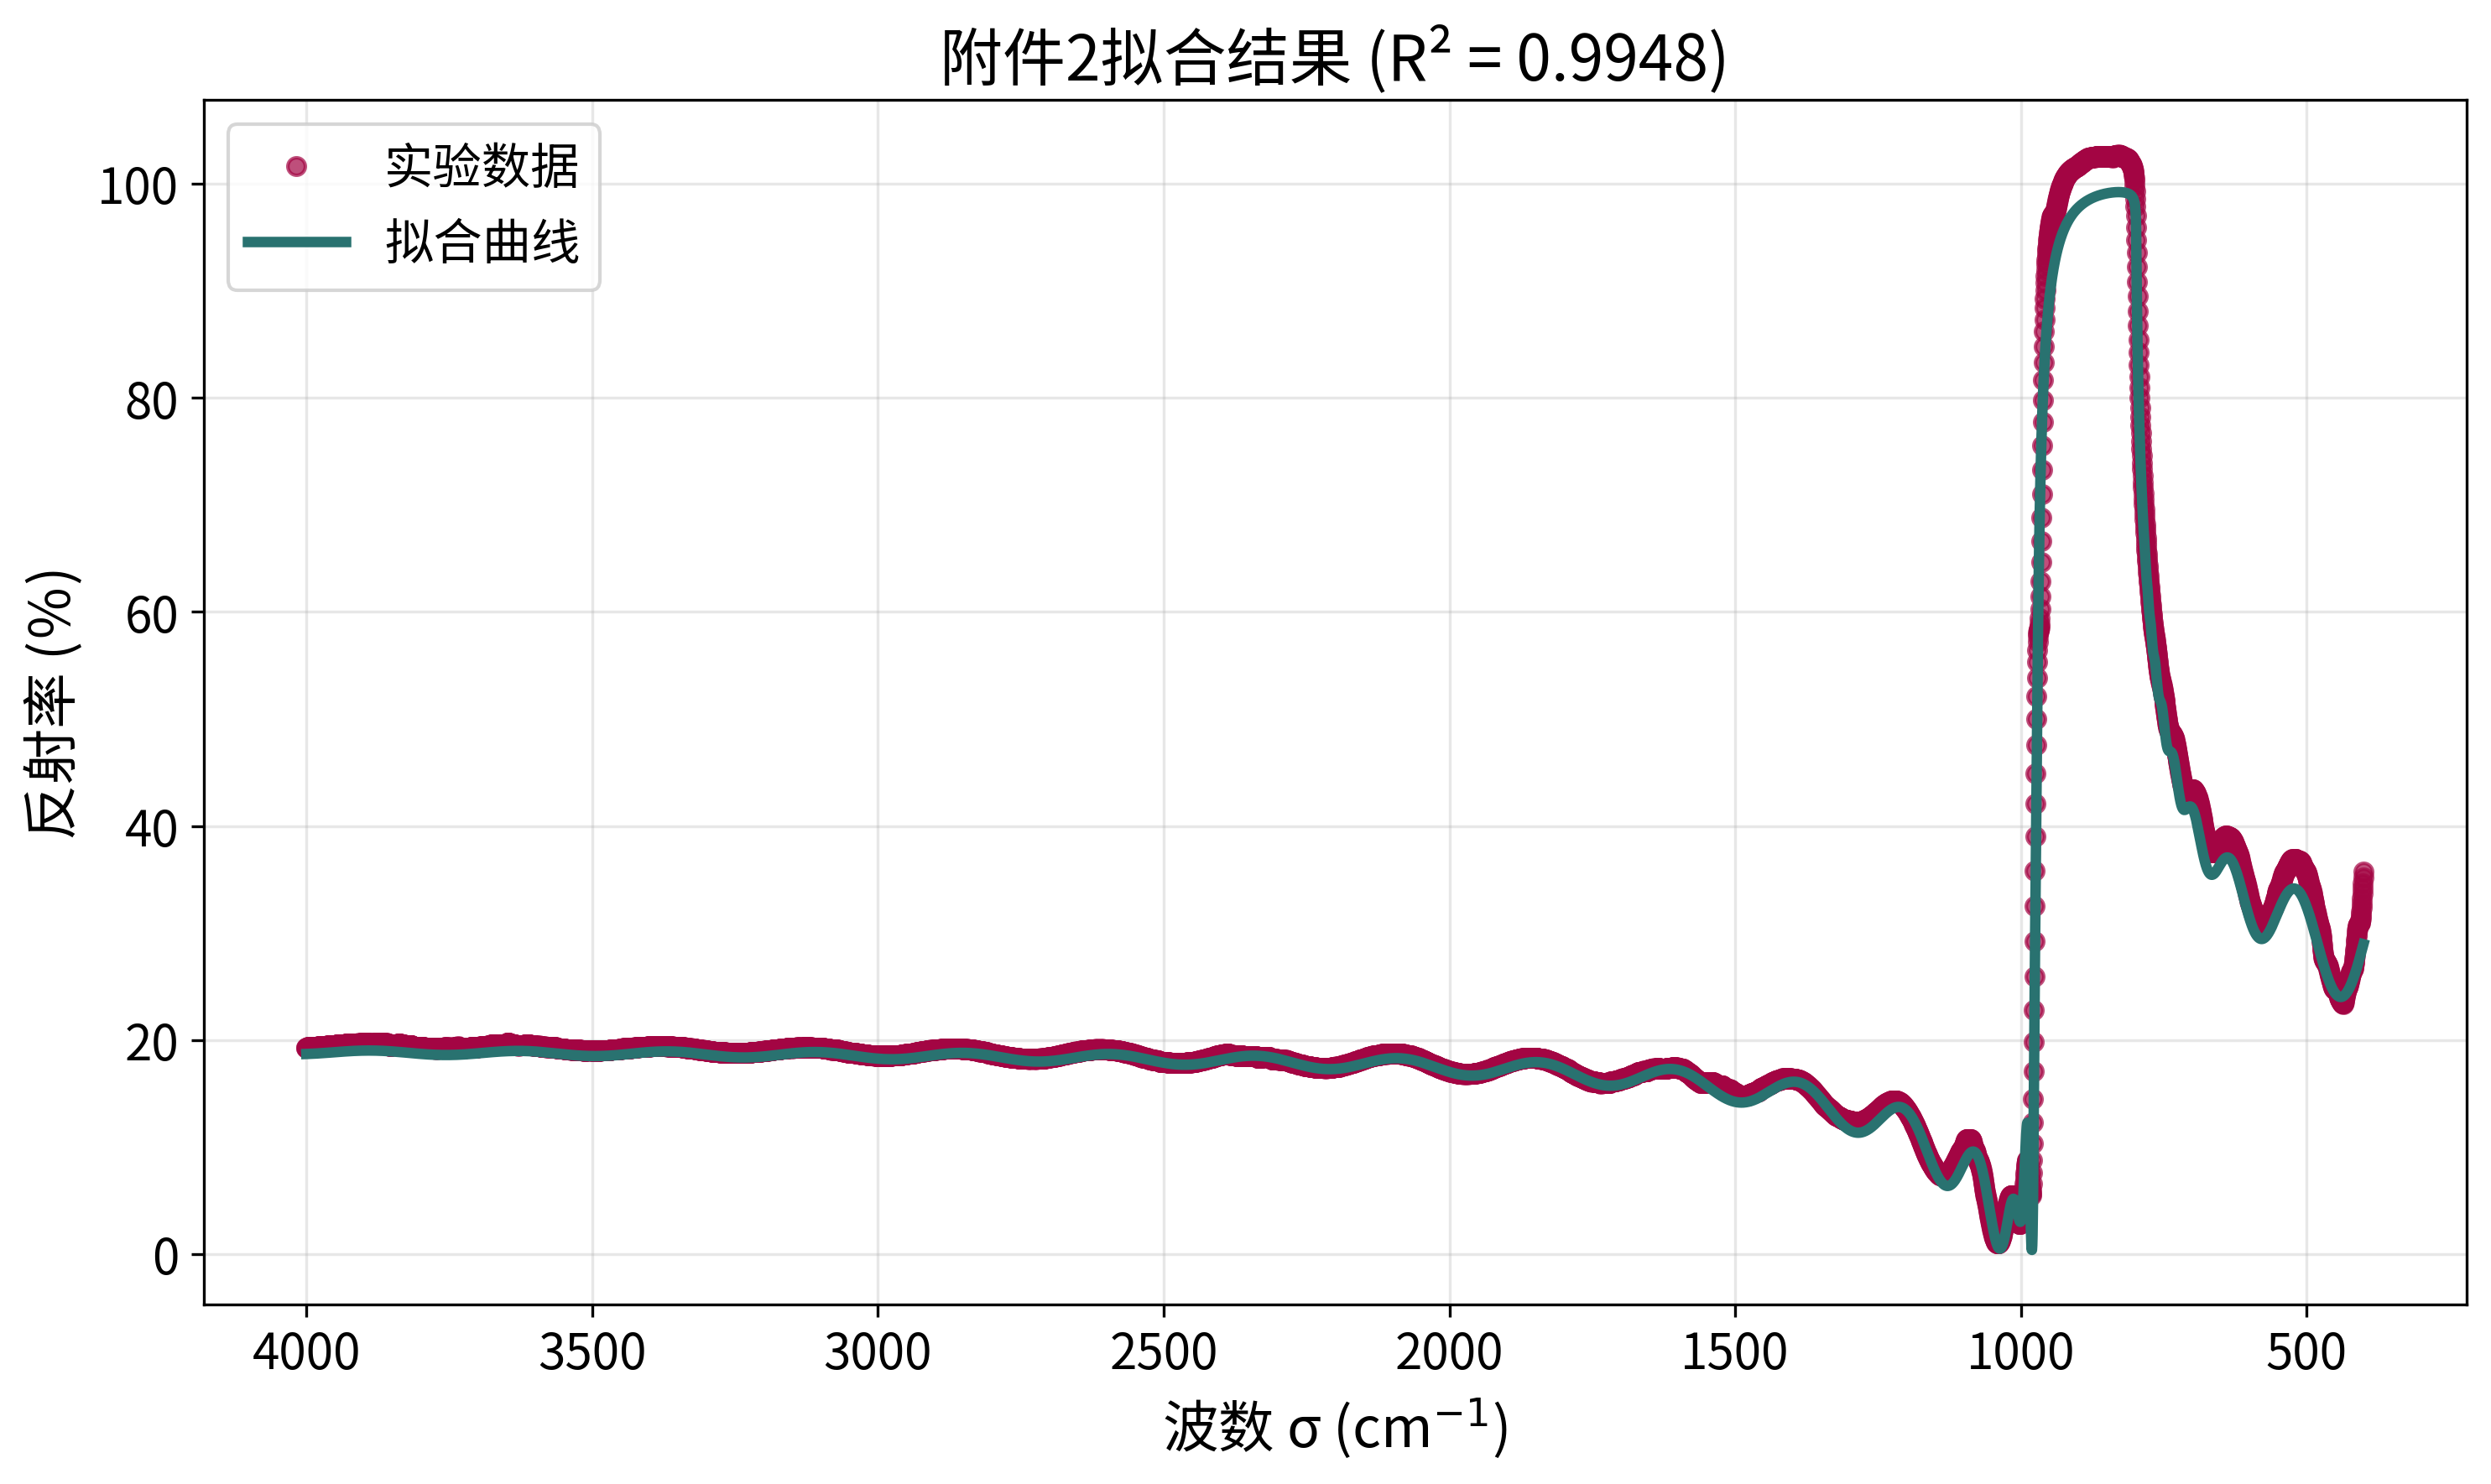
\includegraphics[width=\textwidth]{附件2拟合.png}
%     \caption{附件2全光谱范围的全局同步拟合结果（R²=0.9948）}
%     \label{fig:full_range_plot2}
%   \end{subfigure}

  % --- 整个并排图的总标题和总标签 ---
%   \caption{FFT算法的灵敏度与收敛性综合分析}
%   \label{fig:sensitivity_combined}
% \end{figure}
\subsubsection{模型合理性分析与多光束干涉判断}
为了验证我们所选双光束模型的合理性，我们基于表 \ref{tab:full_range_fit} 中的参数组，计算了外延层和衬底的复折射率，如图（\ref{fig:refractive_index_plot}）所示。

\begin{figure}[h!]
    \centering
    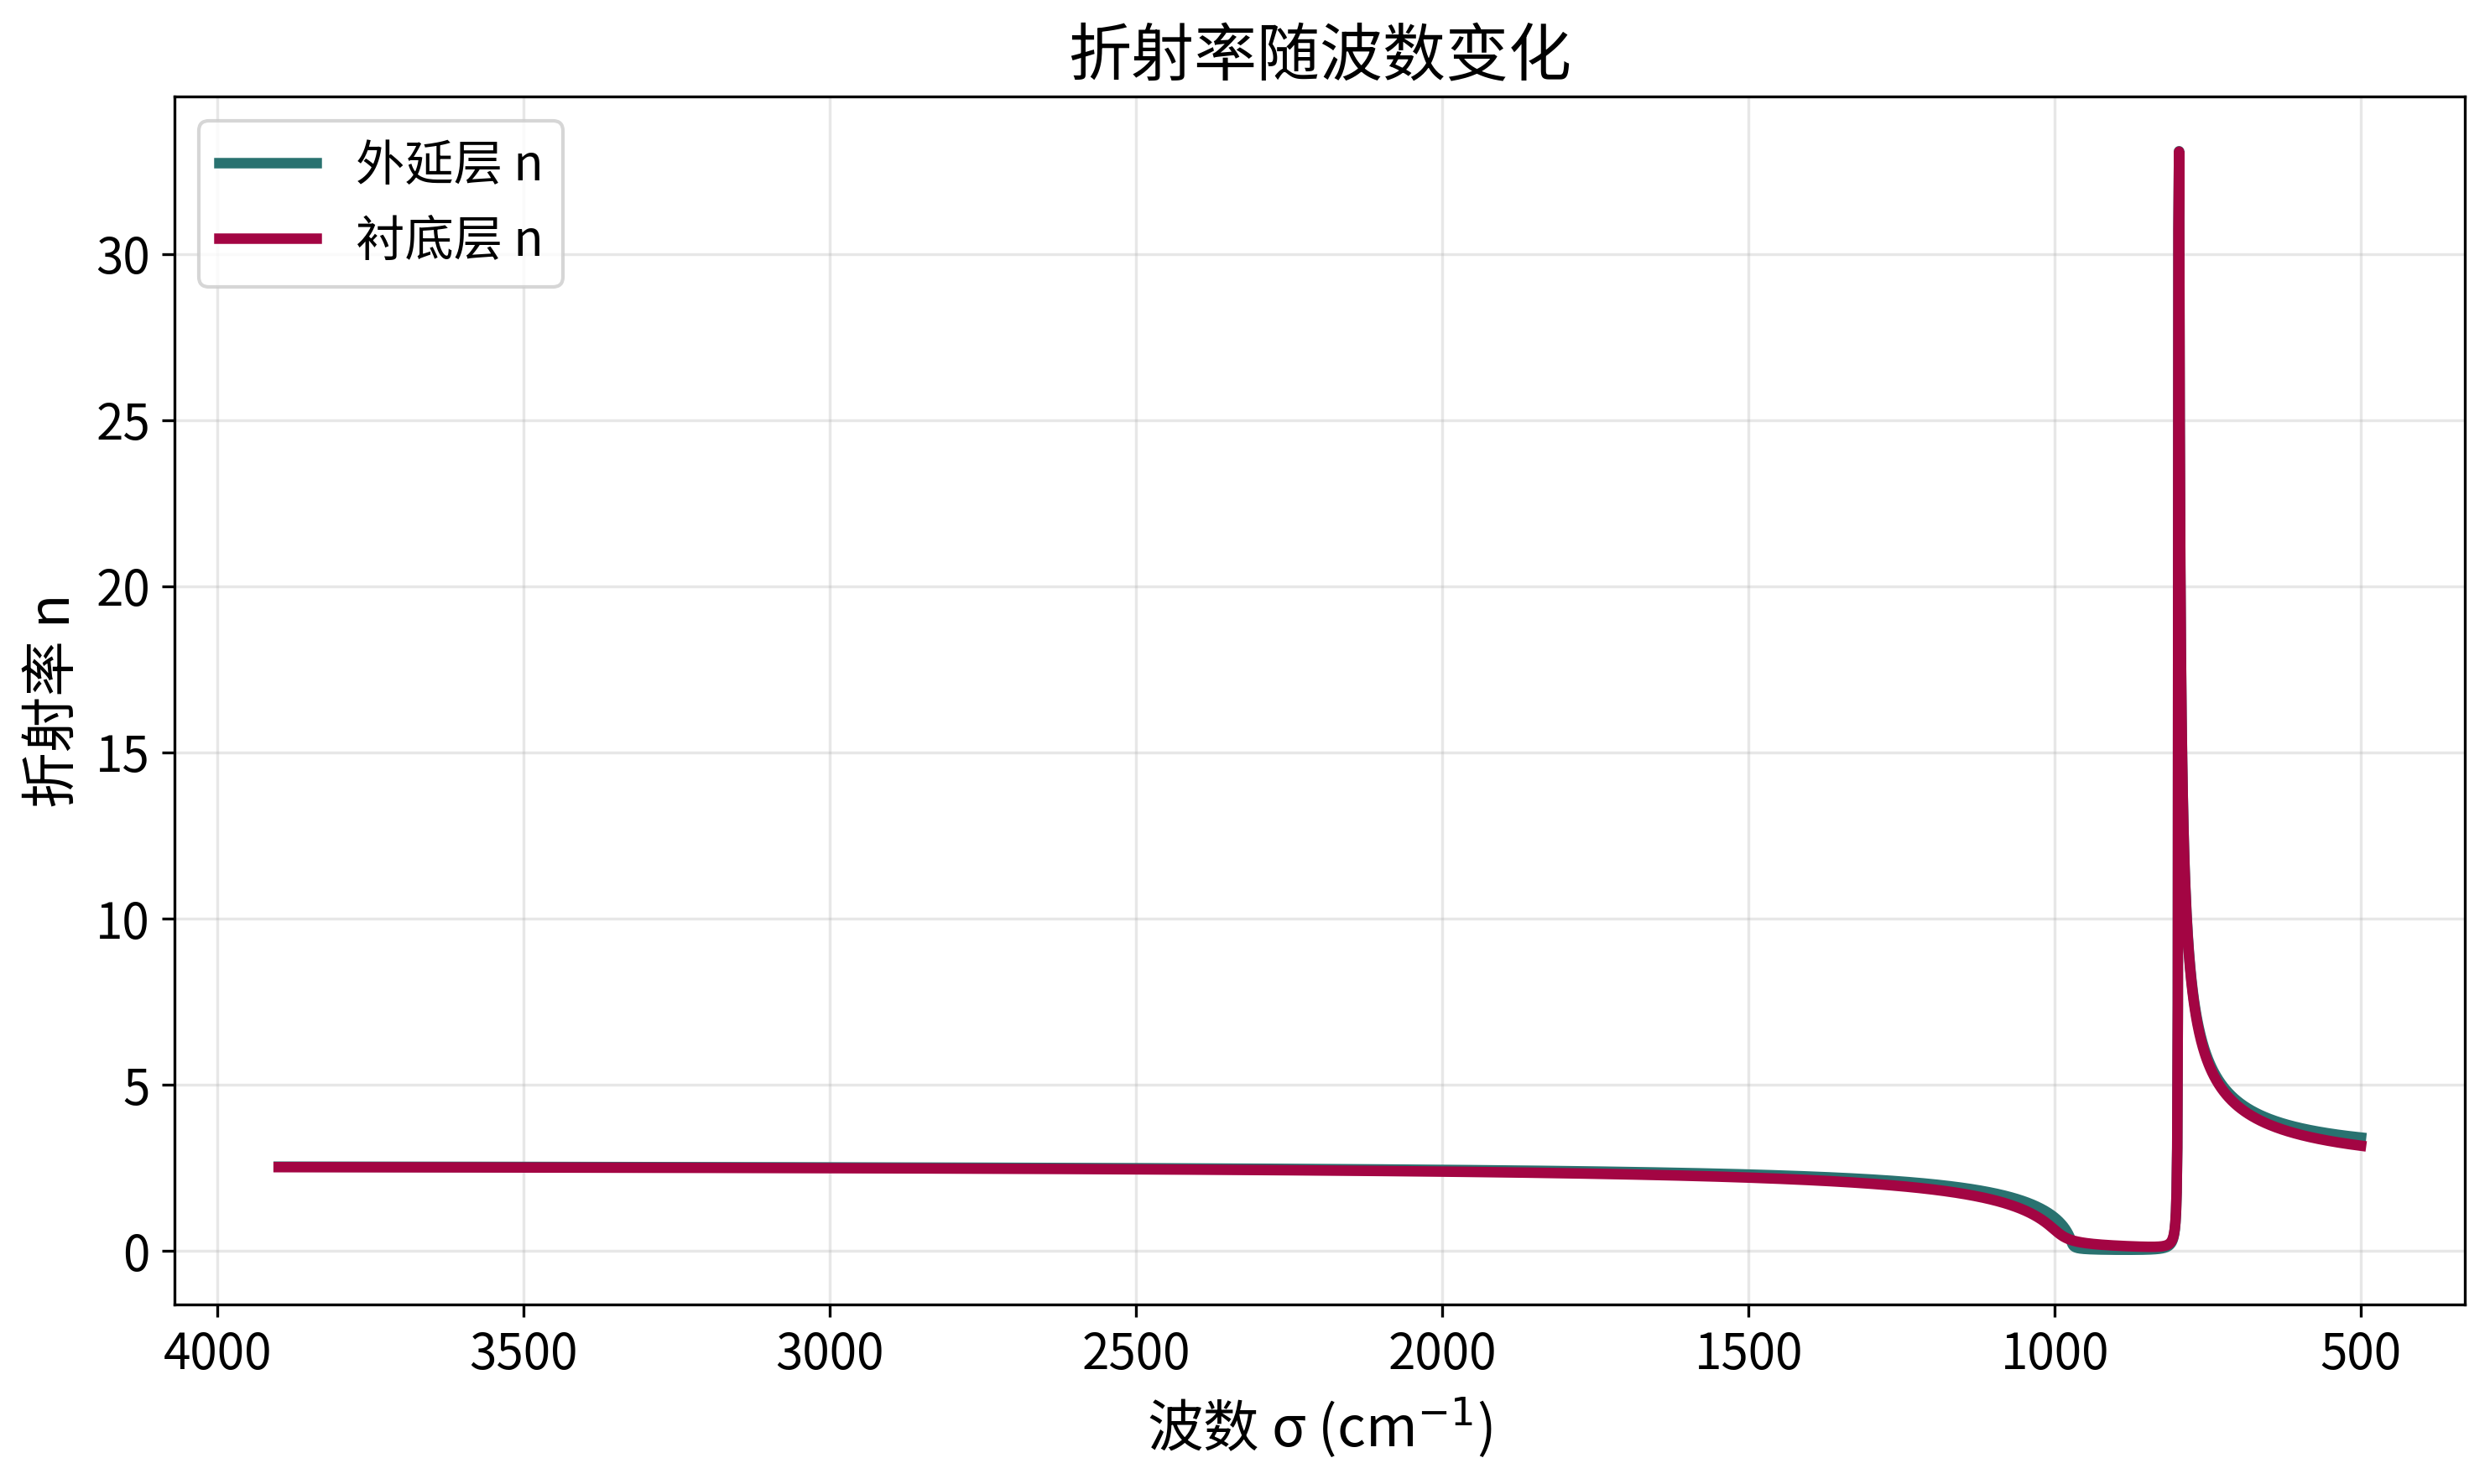
\includegraphics[width=0.7\textwidth]{折射率变化.png}
    \caption{根据最终拟合参数计算得到的外延层与衬底的复折射率谱。}
    \label{fig:refractive_index_plot}
\end{figure}
我们从图（\ref{fig:refractive_index_plot}）中可以发现，在整个光谱范围内，外延层和衬底的折射率实部（n）几乎一致。根据菲涅尔方程，光在两种介质界面处的反射强度主要由二者折射率的差异决定。当 $n_1 \approx n_2$ 时，后续光束在经历多次弱界面反射后，其强度会迅速衰减至可以忽略不计，因此对于本问题中的碳化硅样品，我们可以忽略多光束干涉效应，可以采用\textbf{双光束干涉模型}这一物理模型。


\subsubsection{最终结论与可靠性分析}

基于以上分析，我们忽略了碳化硅样品的多光束干涉效应，采用更合理的双光束干涉模型。所以我们基于问题一模型计算出的厚度 \SI{7.413}{\micro\meter}即为最终结果，无需进行额外修正。

对于最终结果，我们分析其可靠性：
% \begin{enumerate}
%     \item \textbf{模型的物理合理性：} 如上一节所述，通过对拟合参数的物理性质分析，我们验证了双光束干涉模型对于本样品的适用性，证明了我们选择的物理模型是可靠的。

%     \item \textbf{拟合方法的鲁棒性：} 方法成功地在两个数据集上均获得了超过0.99的决定系数（R²），这表明我们的拟合结果有很强的统计可靠性和物理自洽性。

%     \item \textbf{核心参数的稳定性：} 我们绘制了拟合残差图，如图（\ref{fig:residual_plot1}）和（\ref{fig:residual_plot2}）。
%     残差图显示，在波数大于 \SI{1000}{cm^{-1}} 的区域，残差极小，表明模型在此区域的拟合近乎完美。查阅文献\cite{shokhovets2011infrared}后,我们认为残差图在低波数段的系统性偏差，并非简单的模型缺陷，而是高掺杂SiC衬底中LO声子-等离激元耦合（LOPC）现象的外显。
% \end{enumerate}
我们设计的算法成功在附件1和2的数据上获得了超过0.99的决定系数（R²），说明我们的拟合结果有很强的精确度；我们绘制了拟合残差图，如图（\ref{fig:residual_plot1}）和（\ref{fig:residual_plot2}），在波数大于 \SI{1000}{cm^{-1}} 的区域，残差极小，表明模型在此区域的拟合效果很好。所以我们可以认为我们现有模型拟合出来的结果是可靠的。

\begin{figure}[H]
        \centering
        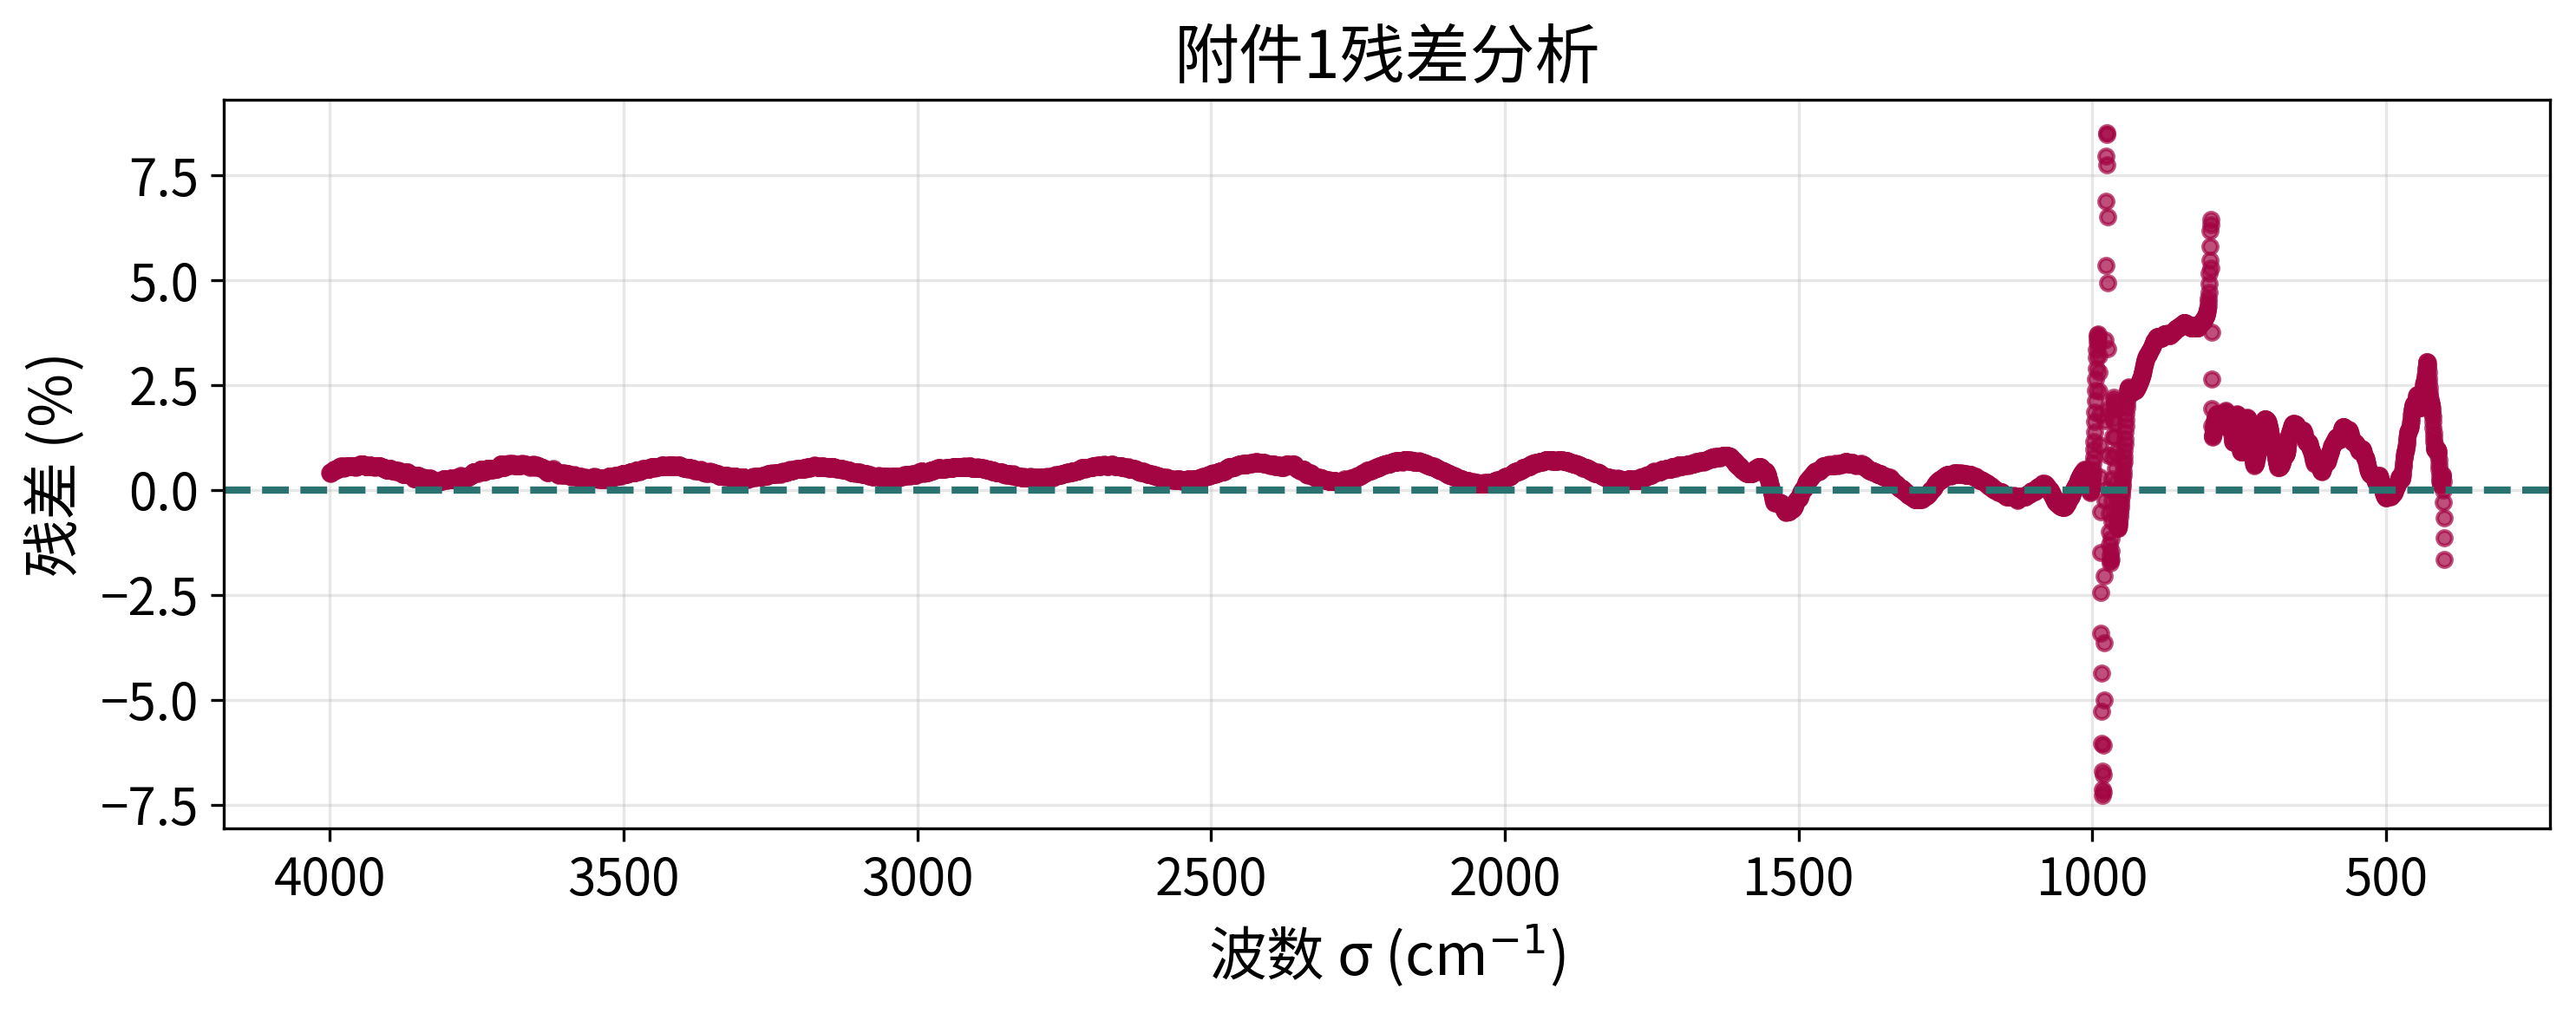
\includegraphics[width=0.7\textwidth]{残差1.png}
        \caption{全光谱拟合中附件1的残差分布图。}
        \label{fig:residual_plot1}
    \end{figure}
    \begin{figure}[H]
        \centering
        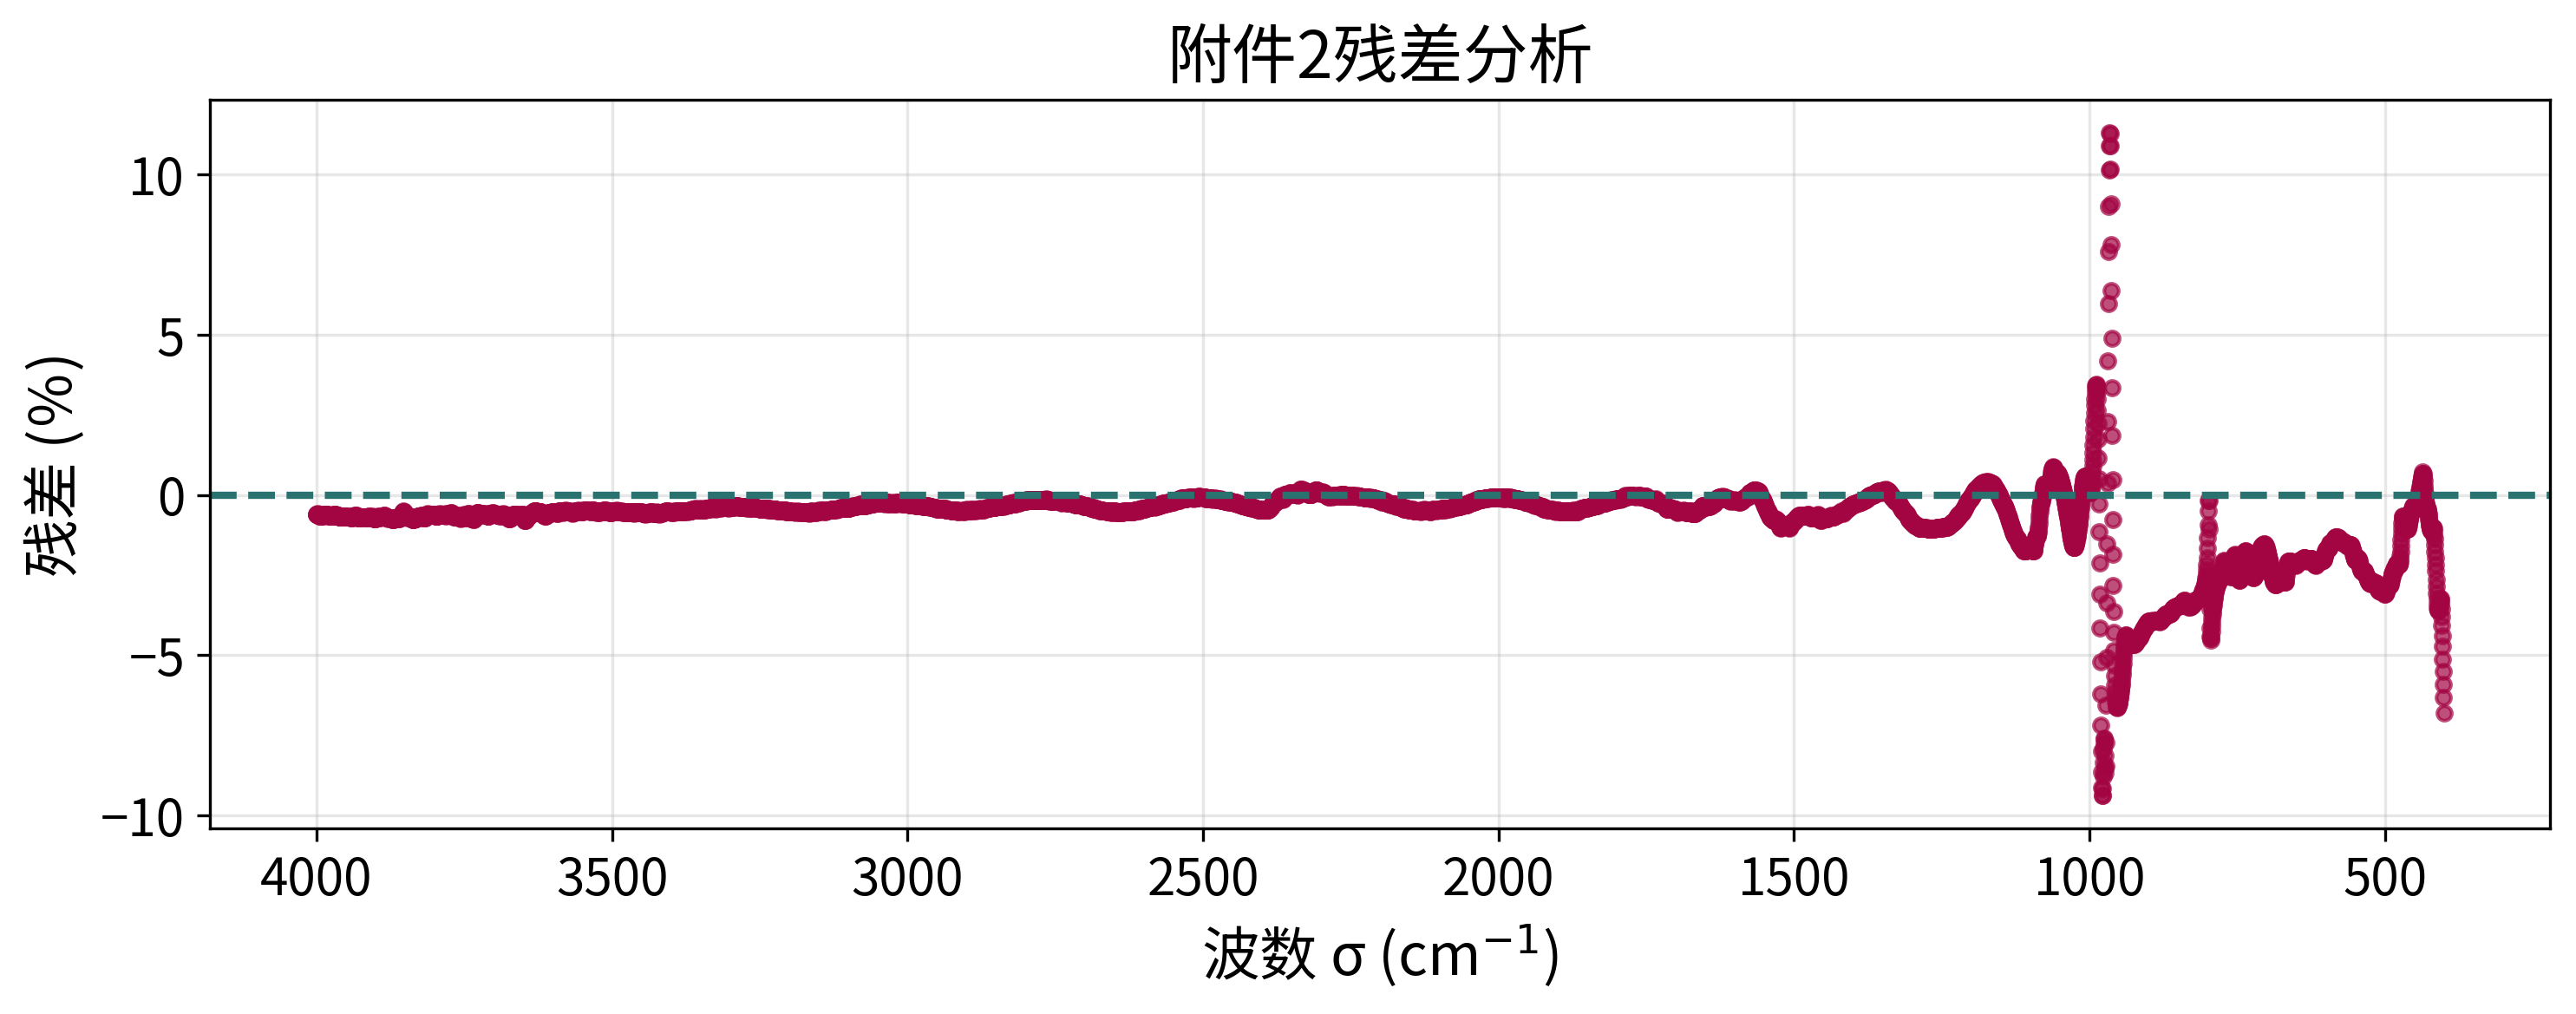
\includegraphics[width=0.7\textwidth]{残差2.png}
        \caption{全光谱拟合中附件2的残差分布图。}
        \label{fig:residual_plot2}
    \end{figure}


当然，如上图所示，模型在低波数区域残差较大，这引发了我们对洛伦兹-德鲁德模型拟合碳化硅衬底的精确性的怀疑。查阅文献\cite{shokhovets2011infrared}后,我们认为残差图在低波数段的系统性偏差，并非简单的模型缺陷，而是高掺杂SiC衬底中LO声子-等离激元耦合（LOPC）现象的外显。


% 综上所述，我们通过一个物理上合理、方法上鲁棒、并且结果经得起检验的流程，确定了外延层的厚度。因此，我们认为计算结果 \textbf{\SI{7.413}{\micro\meter}} 是高度可靠的。


\section{问题三模型的建立与求解}
为了分析硅晶原片的测试结果是否出现多光束干涉，并计算出硅外延层的厚度，我们考虑一个由“空气-外延层-衬底”构成的Fabry–Pérot腔。该模型基于多光束干涉的经典理论和菲涅尔公式对反射率进行计算，并引入了针对硅晶体色散特性的折射率模型。
\subsection{干涉模型：多光束干涉的数学描述}
考虑光在外延层界面和衬底界面产生多次反射和透射，进行相干叠加的结果。

\begin{figure}[h!]
\centering
\begin{minipage}{0.6\textwidth}
    \centering
    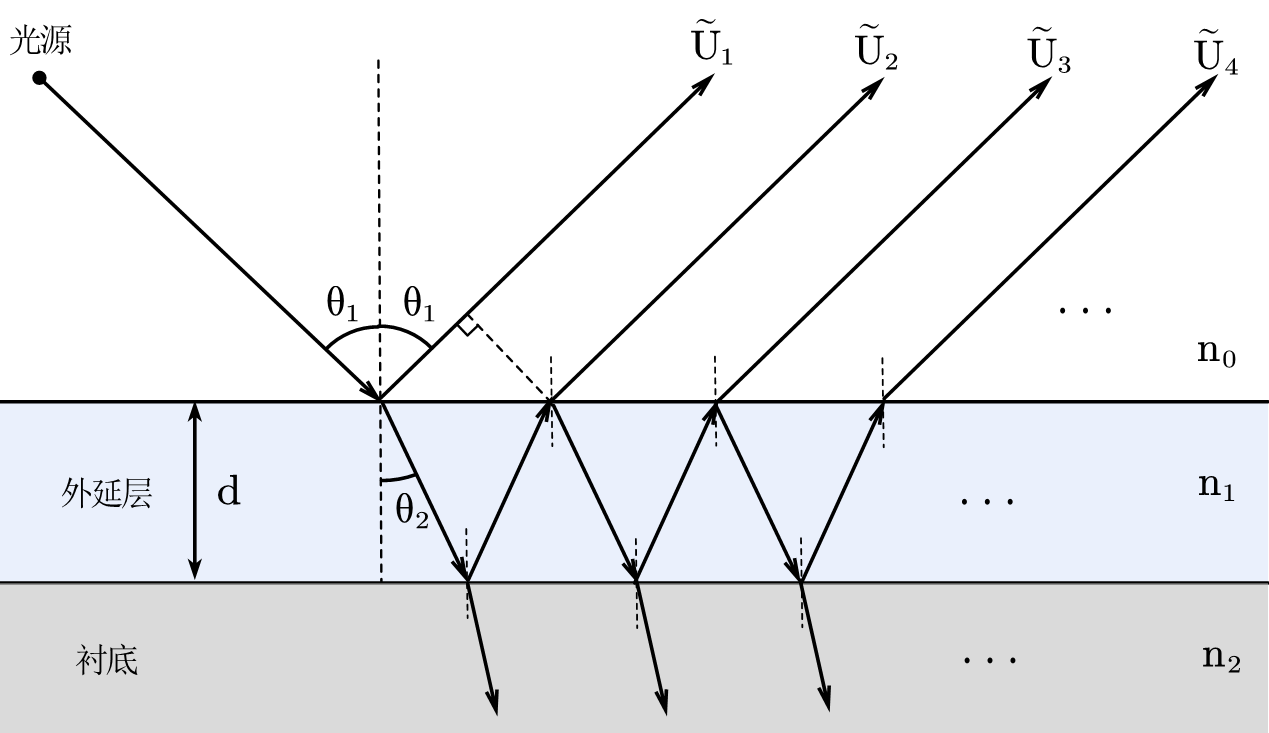
\includegraphics[width=\textwidth]{多光束光路图.png}
    \caption{多光束干涉光路图}
\end{minipage}\hfill
\begin{minipage}{0.35\textwidth}
    \hspace{1.5em} 各级反射光复振幅表达式：
    \begin{equation*}
    \begin{cases}
        \tilde{U}_1 = r_1 A_0, \\[6pt]
        \tilde{U}_2 = r_2 (t_1 t_1') e^{-i\delta} A_0, \\[6pt]
        \tilde{U}_3 = r_2^{2}r_1' (t_1 t_1') e^{-i(2\delta)} A_0, \\[6pt]
        \tilde{U}_4 = r_2^{3}r_1'^2 (t_1 t_1') e^{-i(3\delta)} A_0, \\[6pt]
        \vdots
    \end{cases}
    \end{equation*}
\end{minipage}
\end{figure}

对所有复振幅求和，并带入互易关系$t_1t_1' - r_1r_1' = 1$得到：
\begin{equation}
    \tilde{U}_R =  \left( \frac{r_1 + r_2 e^{- i \delta}}{1 + r_1 r_2 e^{- i \delta}} \right)A_0
\end{equation}

对s光和p光分别计算:
\begin{equation}
    \tilde{U_{s}} = \left( \frac{r_{1s} + r_{2s} e^{- i \delta}}{1 + r_{1s} r_{2s} e^{- i \delta}} \right)A_0
\end{equation}
\begin{equation}
    \tilde{U_{p}} = \left( \frac{r_{1p} + r_{2p} e^{- i \delta}}{1 + r_{1p} r_{2p} e^{- i \delta}} \right)A_0
\end{equation}

二者非相干叠加，得到光强，计算总反射率：
\begin{equation}
    R = \frac{\left| \frac{r_{1s} + r_{2s} e^{- i \delta}}{1 + r_{1s} r_{2s} e^{- i \delta}} \right|^{2} + \left| \frac{r_{1p} + r_{2p} e^{- i \delta}}{1 + r_{1p} r_{2p} e^{- i \delta}} \right|^{2}}{2}  
\end{equation}

\subsection{发生多光束干涉的必要条件}
\subsubsection{相干性条件}
由于现实情况下光的相干长度有限，如果要发生多光束干涉，需要相干长度远大于在介质中往返一次的光程差，这样才能保证同一列光波能在经过多次反射后仍能和自身发生干涉。
\begin{equation}
    L_c >> 2ndcos\theta
\end{equation}

\subsubsection{反射率与吸收条件}
考虑第k次反射波的振幅和第k+1次反射波振幅：
\begin{equation}
    \tilde{U}_k = r_2^{k-1}r_1'^{k-2} (t_1 t_1') e^{-i(k-1)\delta} A_0
\end{equation}
\begin{equation}
    \tilde{U}_{k+1} = r_2^{k}r_1'^{k-1} (t_1 t_1') e^{-i(k)\delta} A_0
\end{equation}

计算(k+1)次反射光和k次反射光振幅比，得到：
\[
\begin{cases}
\left|\frac{\tilde{U}_{1}}{\tilde{U}_2}\right| = \left|\frac{r_2t_1t_1'e^{-i\delta}}{r_1}\right| & k = 1 \\[6pt]
\left|\frac{\tilde{U}_{k+1}}{\tilde{U}_k}\right| = \left|r_1'r_2e^{-i\delta} \right|  & k \geq 2
\end{cases}
\]

若要发生多光束干涉，需要满足经过多次透射折射后的反射光振幅衰减较慢。

在这里，我们认为如果:
\begin{equation}
    \left|r_1'r_2e^{-i\delta} \right| \sim 10^{-1} \text{-} 10^{0}
\end{equation}

则多次反射光对于最终光强仍有较大贡献，需要考虑多光束产生的影响。

若:
\begin{equation}
    \left|r_1'r_2e^{-i\delta} \right| <<1
\end{equation}

则多次反射波的振幅衰减极快，对光强的影响将小于数据噪音，可以忽略，只需考虑双光束干涉。

\subsubsection{几何与均匀性条件}
两界面基本平行且足够光滑，膜层厚度在光斑内均匀，这样相邻往返的相位差保持恒定值:
\begin{equation}
    \delta = \frac{4 \pi n d \cos \theta}{\lambda}
\end{equation}

% \subsection{发生多光束干涉的反射率随波数变化特征}

% 反射率公式可化简为:
% \begin{equation}
%     R = 1 
%     - \frac{(r_{1s}r_{2s})^2 + 1 - r_{1s}^2 - r_{2s}^2}{2\bigl(1 + (r_{1s}r_{2s})^2 + 2r_{1s}r_{2s}\cos\delta\bigr)}
%     - \frac{(r_{1p}r_{2p})^2 + 1 - r_{1p}^2 - r_{2p}^2}{2\bigl(1 + (r_{1p}r_{2p})^2 + 2r_{1p}r_{2p}\cos\delta\bigr)}
%     \label{R}
% \end{equation}


% \begin{equation}
%     \delta = 4\pi ndcos\theta \sigma
%     \label{distance}
% \end{equation}

\subsection{多光束干涉对厚度计算精度的影响分析}
\subsubsection{对比度分析}
对比度V是衡量波峰和波谷光强变化相对于本底光强的明显程度的物理量，它的定义是：
\begin{equation}
    V = \frac{I_{max} - I_{min}}{I_{max} + I_{min}}
\end{equation}
通过波动图像的峰值推算厚度d，对比度越大，波峰和波谷越明显，对峰值处的波数值测量更准确。反之，如果对比度很小，峰值测量误差大，会导致最终算出的d存在较大误差。

对于双光束干涉，若两束光的强度分别为$I_1$,$I_2$,二者相位差为$\delta$则对比度由公式：
\begin{equation}
    V_{2beam} = \frac{2\sqrt{I_1I_2}}{I_1 + I_2}
\end{equation}
对多光束干涉，若衬底和空气折射率差异不大，可近似使用经典 Airy 公式给出透射强度：
\begin{equation}
T(\delta) = \frac{1}{1 + F \sin^{2}\!\left(\tfrac{\delta}{2}\right)}, 
\qquad 
F = \frac{4R}{(1 - R)^{2}} \, .
\end{equation}
得到对比度为：
\begin{equation}
    V_{multi} = \frac{F}{F+2}
\end{equation}

在通常情况下$V_{multi} >> V_{2beam}$,若发生多光束干涉，能使条纹对比度更大，测量和标定的峰值坐标更加准确，厚度计算精度更高。

\subsubsection{精细度分析}
    光谱精细度F是衡量干涉条纹尖锐程度的物理量，由文献 [3]，精细度被定义为干涉条纹的自由光
谱范围（FSR, Free Spectral Range）与半高全宽（FWHM, Full Width at Half Maximum）的比值：
    \begin{equation}
        F = \frac{FSR}{FWHM} = \frac{\Delta\sigma}{\delta \sigma}
        \label{fitness}
    \end{equation}
    光谱精细度F越大，波峰越锐利，对波峰处数值的定位和测量更加准确。
对于双光束干涉，其干涉条纹呈余弦分布，由定义计算：
\begin{equation}
    F_{2beam} \approx 2
\end{equation}
对多光束干涉，谱线会出现明显的锐利尖峰,在合适条件下F会远大于2:
\begin{equation}
    F_{multi} > 2
\end{equation}
若发生多光束干涉，其干涉条纹在频谱上更加锐利，对峰值的定位更加准确，厚度计算精度更高。

\subsection{对硅晶圆片发生多光束干涉的定性判断}
% \subsubsection{定性分析}

对于双光束干涉，可以得到峰值间隔$\Delta \sigma \approx \frac{1}{2ndcos\theta}$，将反射率R的表达式抽象为函数形式:
\begin{equation}
    R(\sigma) = A_1(\sigma) + B_1(\sigma)cos(C_1\sigma)
\end{equation}

若发生多光束干涉，峰值之间的波数间隔$\Delta \sigma \approx \frac{1}{2ndcos\theta}$
与双光束一致，对于R的表达式，可以抽象为函数形式:
\begin{equation}
    R(\sigma) = 1 - \frac{A_2(\sigma)}{B_2(\sigma) + C_2(\sigma)cos(D_2\sigma)}
\end{equation}
为考察其波动特征，可以先忽略振幅调制，只考虑相位对反射率图像的影响，取合适参数作图：
\begin{figure}[h!]
\centering
\begin{minipage}{0.45\textwidth}
    \centering
    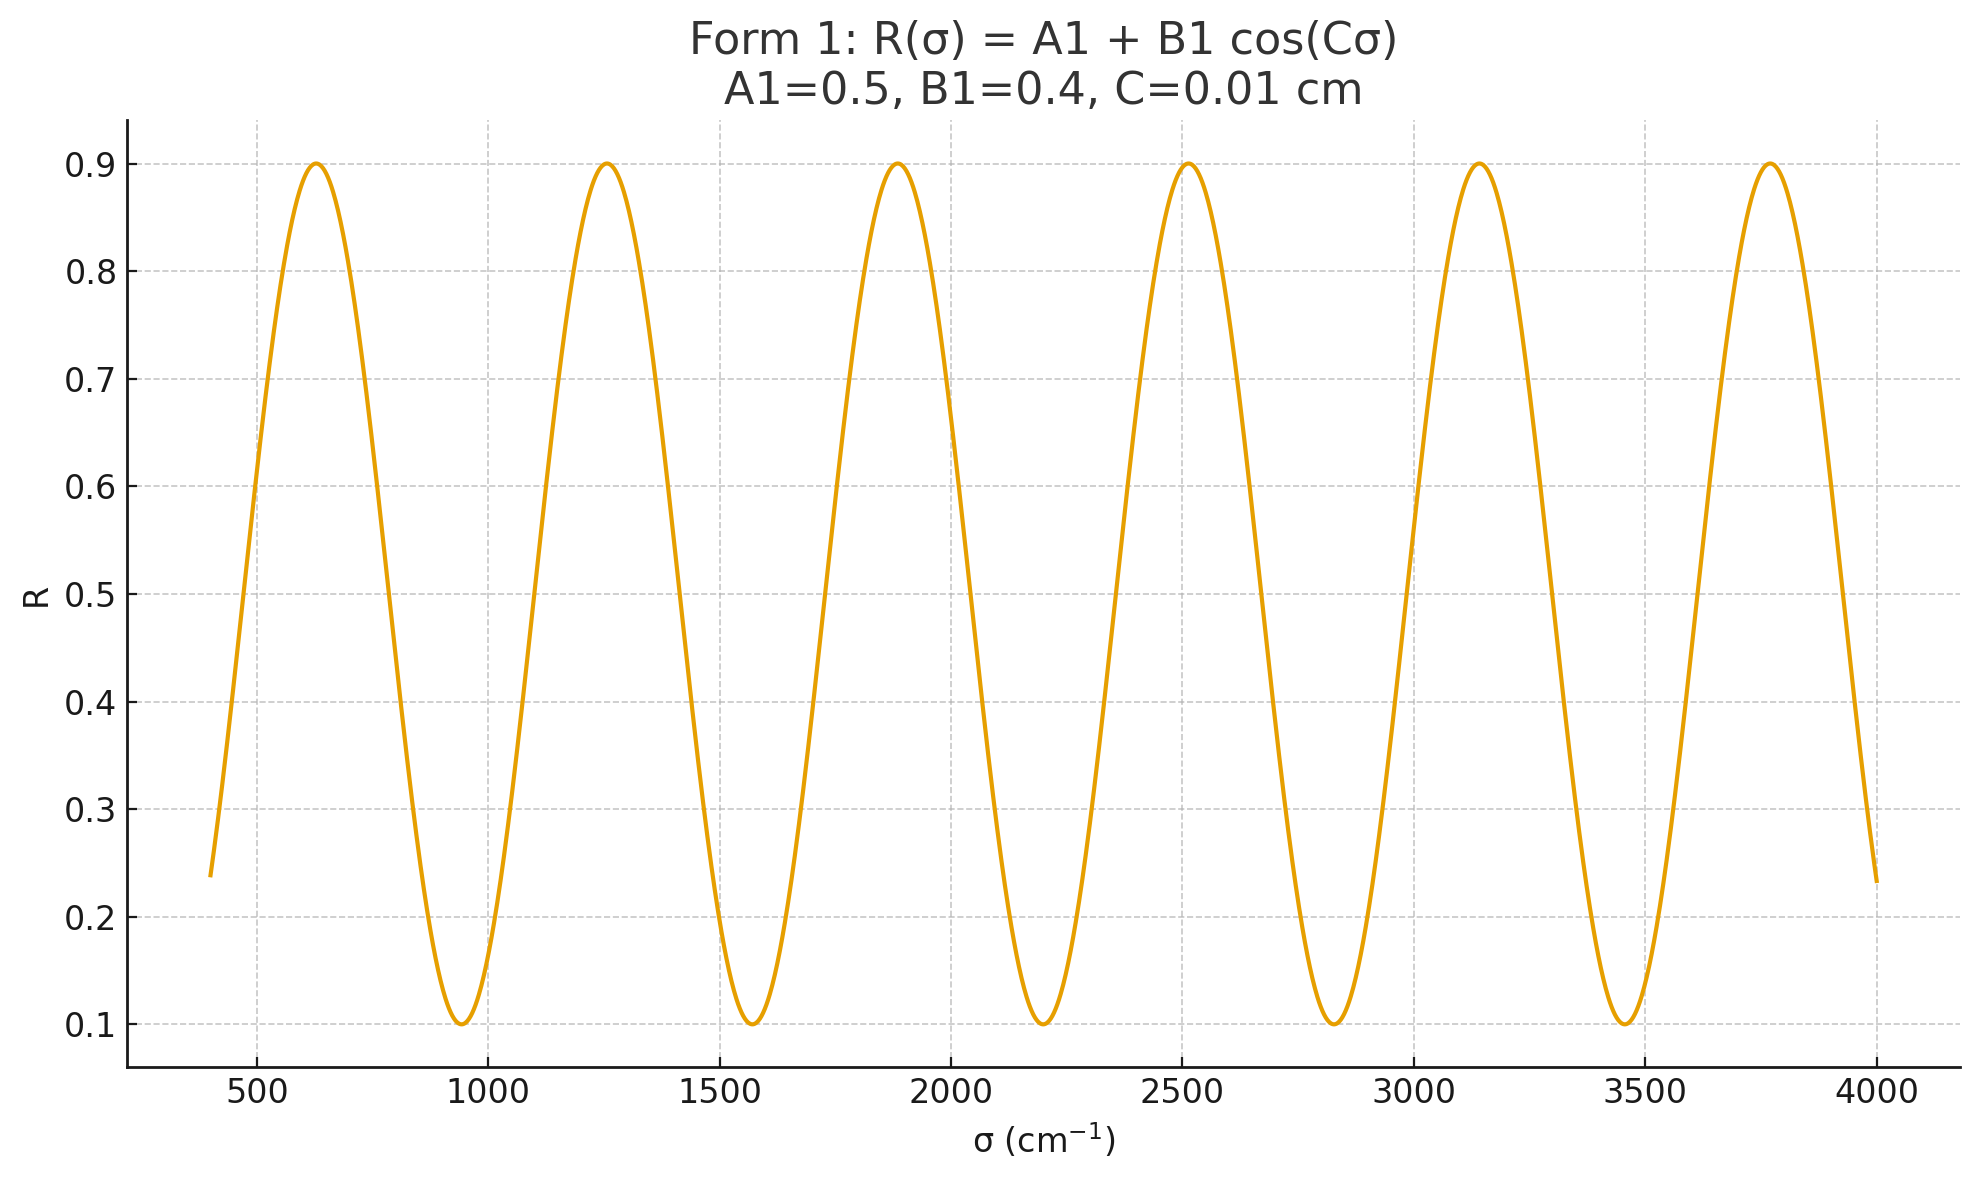
\includegraphics[width=\textwidth]{定性图_多光束.png}
    \caption{双光束干涉反射率形貌图}
    \label{fig:1}
\end{minipage}
\hfill
\begin{minipage}{0.45\textwidth}
    \centering
    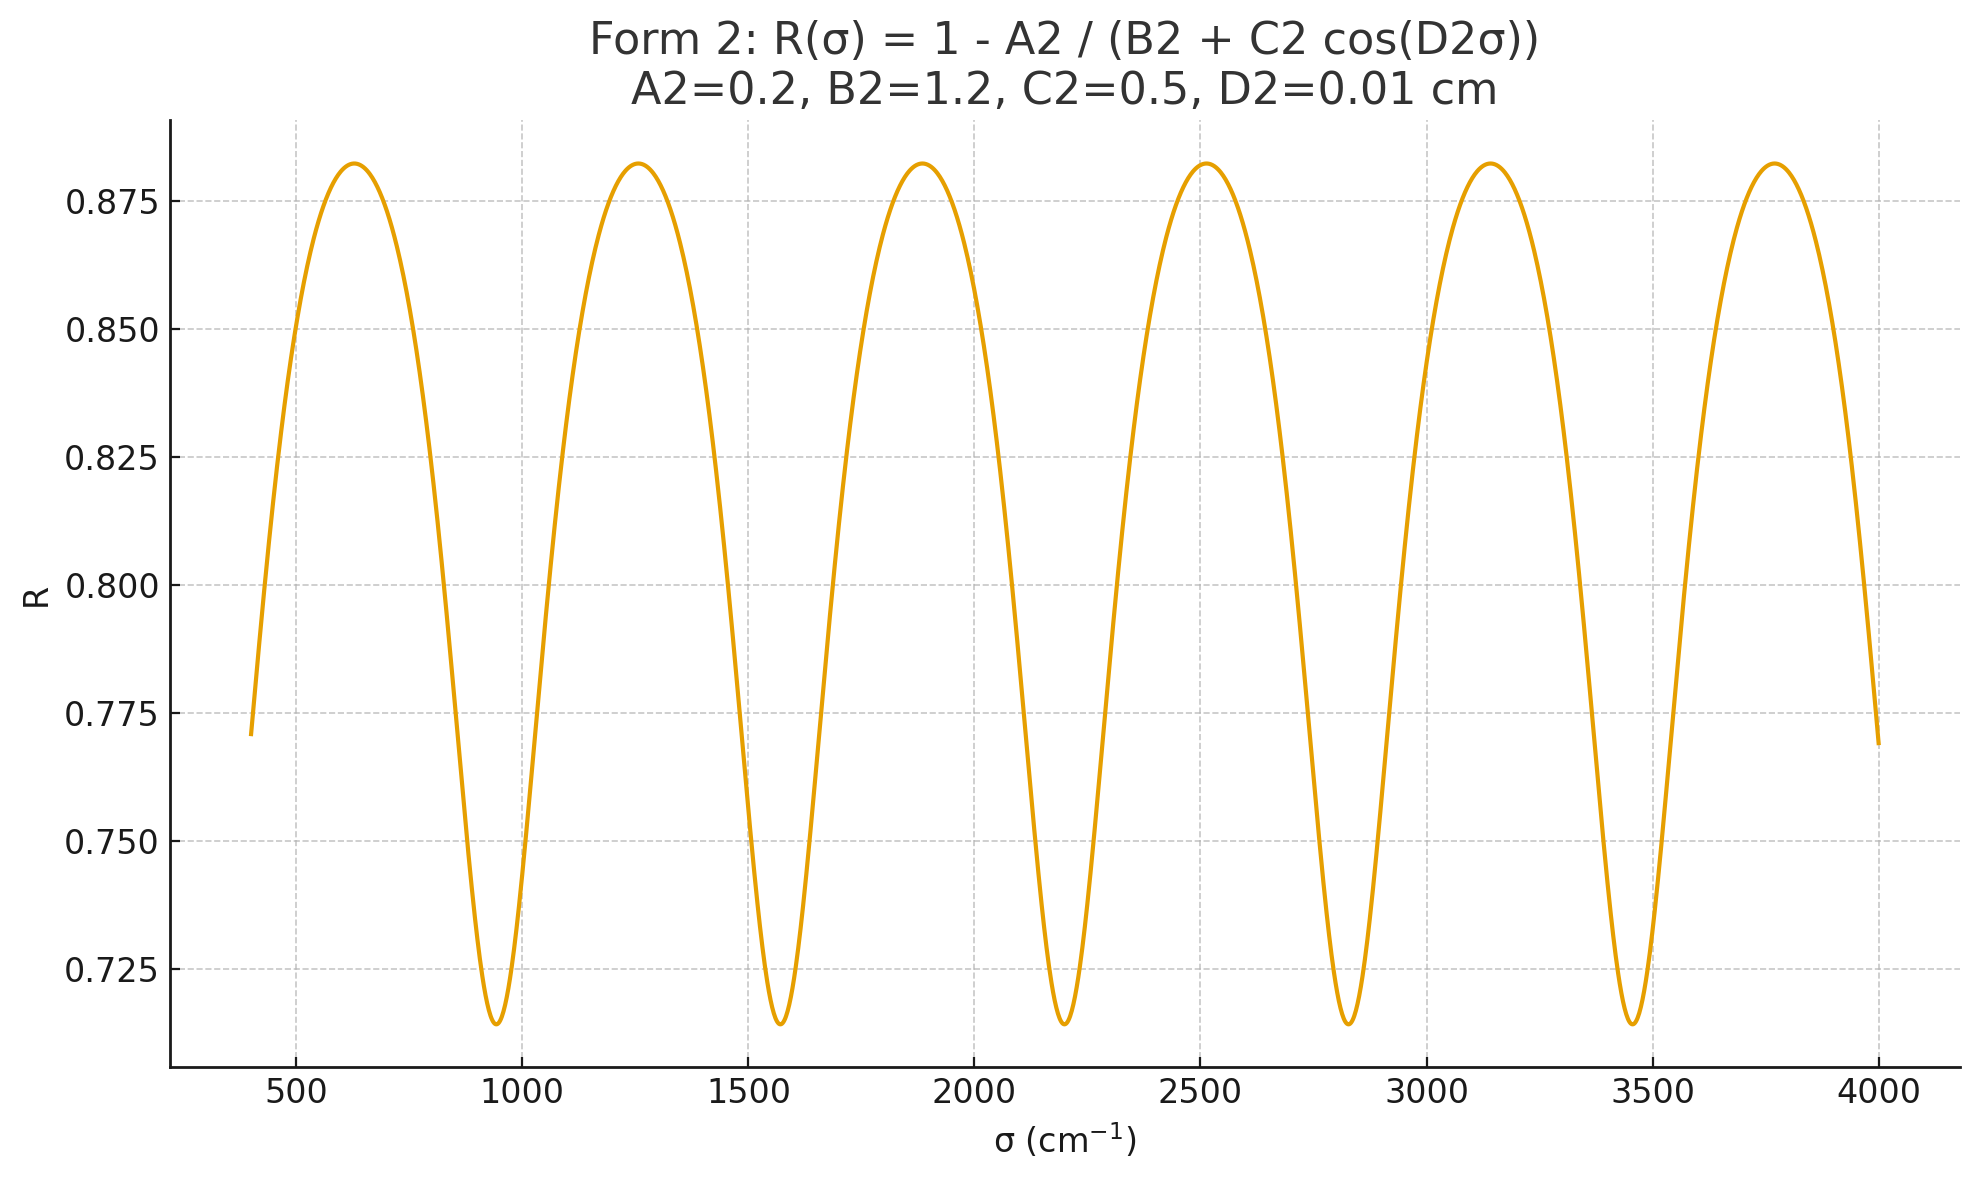
\includegraphics[width=\textwidth]{定性图_双光束.png}
    \caption{多光束干涉反射率形貌图}
    \label{fig:2}
\end{minipage}
\end{figure}

对比发现，双光束干涉的波峰和波谷基本对称。而多光束呈现出波峰较圆，波谷较尖的特征，与附件3，4图像中出现的波峰波谷非对称现象相符。

据此，可以定性推断附件 3 和附件 4 提供的硅晶圆片的测试结果出现了多光束干涉。\\


\subsection{基于干涉极值点的外延层厚度数学模型}
在确认附件3和附件4的光谱具有明显的多光束干涉特征后，我们设计了一种基于干涉极值点（波峰与波谷）位置的解析算法来精确求解外延层厚度。
\subsubsection{算法模型选择}
% 问题二中，碳化硅的光学特性复杂，其厚度 $d$ 与载流子浓度 $N$、迁移率 $\mu$ 等多个物理参数相互耦合，须通过全局拟合整个光谱才能准确解耦并求解所有参数。
与问题二不同，问题三的硅晶圆片产生的光谱是由高透明介质产生的\textbf{高保真多光束干涉条纹}，所以其光学响应主要由实部折射率 $n$ 确定。这意味着光谱中反射率仅与厚度 $d$ 存在函数关系，与其他物理参数基本无关。基于此，我们选择\textbf{干涉极值点解析法}。

\subsubsection{折射率模型}
% 经查阅，硅与碳化硅在晶体结构上存在根本性差异：前者不存在永久电偶极矩，其晶格振动在红外波段是\textbf{非一阶红外活性的}，没有强烈的声子共振吸收峰，表现为高度透明；而后者Si-C化学键存在电偶极矩，晶格振动（声子）具有强烈的\textbf{一阶红外活性}，能够在红外波段与光子发生强烈的共振吸收。因此，描述SiC须使用洛伦兹振子项的洛伦兹-德鲁德模型，而Si外延层则须选取其他模型表示折射率。

硅与碳化硅在晶体结构上存在根本差异，其晶格振动在红外波段高度透明，所以我们无法直接沿用问题二的折射率模型。通过使用AI\cite{ai:gemini}进行文献搜索，我们发现对于硅外延层，其在红外波段的折射率色散关系可以通过一个三项的塞尔迈耶方程精确描述。根据文献\cite{li1980refractive}，该方程形式如下：
\begin{equation}
    n_{\text{Si}}^2(\lambda) = 1 + \sum_{j=1}^{3} \frac{B_j \lambda^2}{\lambda^2 - C_j}
    \label{eq:sellmeier_si_3term}
\end{equation}

其中，$n_{\text{Si}}(\lambda)$ 是硅在波长 $\lambda$ 处的折射率。通过阅读文献，我们采用色散系数 $B_j$ 和 $C_j$这一组经验常数 ，其数值如下：
\begin{align*}
    B_1 &= 10.6684293,   &\quad C_1 &= 0.09091219 \, \mu\text{m}^2 \\
    B_2 &= 0.0030434748,  &\quad C_2 &= 1.28766018 \, \mu\text{m}^2 \\
    B_3 &= 1.54133408,    &\quad C_3 &= 1218816    \, \mu\text{m}^2
\end{align*}
\subsubsection{干涉模型}
% 光波在厚度为 $d$、折射率为 $n$ 的薄膜中以角度 $\theta_1$ 传播并往返一次所产生的相位差 $\delta$由公式（\ref{distance}）表示：$\delta = 4\pi ndcos\theta_1 \sigma$。

% 干涉光谱的极值点出现在相位差满足特定条件的位置：
% \begin{itemize}
%     \item \textbf{相长干涉 (波峰)}: $\delta = m \cdot 2\pi$, 其中 $m$ 为整数，称为干涉级数。
%     \item \textbf{相消干涉 (波谷)}: $\delta = (m + 1/2) \cdot 2\pi$, 其中 $m$ 为整数。
% \end{itemize}

% 将以上两式统一，并代入相位差公式，可反解出厚度 $d$ 的计算式：
% \begin{equation}
%     d = \frac{k}{2 n(\sigma_k) \cos\theta_1 \sigma_k}
%     \label{eq:thickness_formula}
% \end{equation}
% 其中，$\sigma_k$ 是第 $k$ 个极值点的波数，$n(\sigma_k)$ 是在该波数下由塞尔迈耶方程计算出的折射率。干涉级数因子 $k$ 对于波峰是整数，对于波谷是半整数。
干涉光谱的极值点（波峰与波谷）满足其相位差 $\delta$ 为 $\pi$ 的整数倍。我们可以将此条件统一表示为 $\delta = k \cdot 2\pi$（k取0.5的整数倍），其中，干涉级数因子 $k$ 对于相长干涉的波峰是整数，对于相消干涉的波谷是半整数。

将相位差的表达式 $\delta = 4\pi n d \cos\theta_1 \sigma$ 代入上式，即可反解出厚度 $d$ 的计算公式：
\begin{equation}
    d = \frac{k}{2 n(\sigma_k) \cos\theta_1 \sigma_k}
    \label{eq:thickness_formula}
\end{equation}
其中，$\sigma_k$ 是对应级数因子为 $k$ 的极值点波数，$n(\sigma_k)$ 是在该波数下由塞尔迈耶方程计算出的折射率。

\subsubsection{算法流程与数据}
\begin{enumerate}
    \item \textbf{数据提取}: 从实验光谱数据中精确提取所有干涉极值点（波峰与波谷）的波数位置 $\sigma_k$。表 \ref{tab:extrema_points} 列出了用于计算的精确数据。
    \item \textbf{遍历搜索}: 设定一个合理的整数范围，遍历尝试第一个极值点的初始干涉级数 $m_0$因子。
    \item \textbf{厚度计算}: 对于每一个假定的 $m_0$，根据所有极值点的相对顺序确定它们的干涉级数序列（例如 $m_0, m_0+0.5, m_0+1, \dots$），并利用公式（\ref{eq:thickness_formula}）计算出一组对应的厚度值 $\{d_k\}$。 
    \item \textbf{确定最优解}: 计算该组厚度值 $\{d_k\}$ 的标准差 $\text{std}(\{d_k\})$。能够使标准差 $\text{std}(\{d_k\})$ 达到最小的 $m_0$ 即为正确的初始干涉级数。该 $m_0$ 对应的厚度平均值 $\bar{d}$ 即为最终求解结果。
\end{enumerate}

\begin{table}[htbp]
\centering
\caption{附件3与附件4光谱的精确极值点数据}
\label{tab:extrema_points}
\begin{minipage}{0.48\textwidth}
    \centering
    \label{tab:data3}
    \subcaption{附件3 (入射角 10°)}
    \begin{tabular}{ccc}
        \toprule
        序号 & 波数 (cm$^{-1}$) & 类型 \\
        \midrule
        1  & 750.17  & 波峰 \\
        2  & 940.61  & 波谷 \\
        3  & 1105.49 & 波峰 \\
        4  & 1312.80 & 波谷 \\
        5  & 1508.06 & 波峰 \\
        6  & 1722.60 & 波谷 \\
        7  & 1927.02 & 波峰 \\
        8  & 2144.94 & 波谷 \\
        \bottomrule
    \end{tabular}
\end{minipage}
\hfill
\begin{minipage}{0.48\textwidth}
    \centering
    \label{tab:data4}
    \subcaption{附件4 (入射角 15°)}
    \begin{tabular}{ccc}
        \toprule
        序号 & 波数 (cm$^{-1}$) & 类型 \\
        \midrule
        1  & 574.20  & 波谷 \\
        2  & 749.21  & 波峰 \\
        3  & 946.40  & 波谷 \\
        4  & 1108.39 & 波峰 \\
        5  & 1324.38 & 波谷 \\
        6  & 1519.15 & 波峰 \\
        7  & 1736.10 & 波谷 \\
        8  & 1941.97 & 波峰 \\
        \bottomrule
    \end{tabular}
\end{minipage}
\end{table}

\subsubsection{计算结果与分析}
\begin{figure}[h]
  \centering
  % 指定图片文件，png/jpg/pdf 都可以
  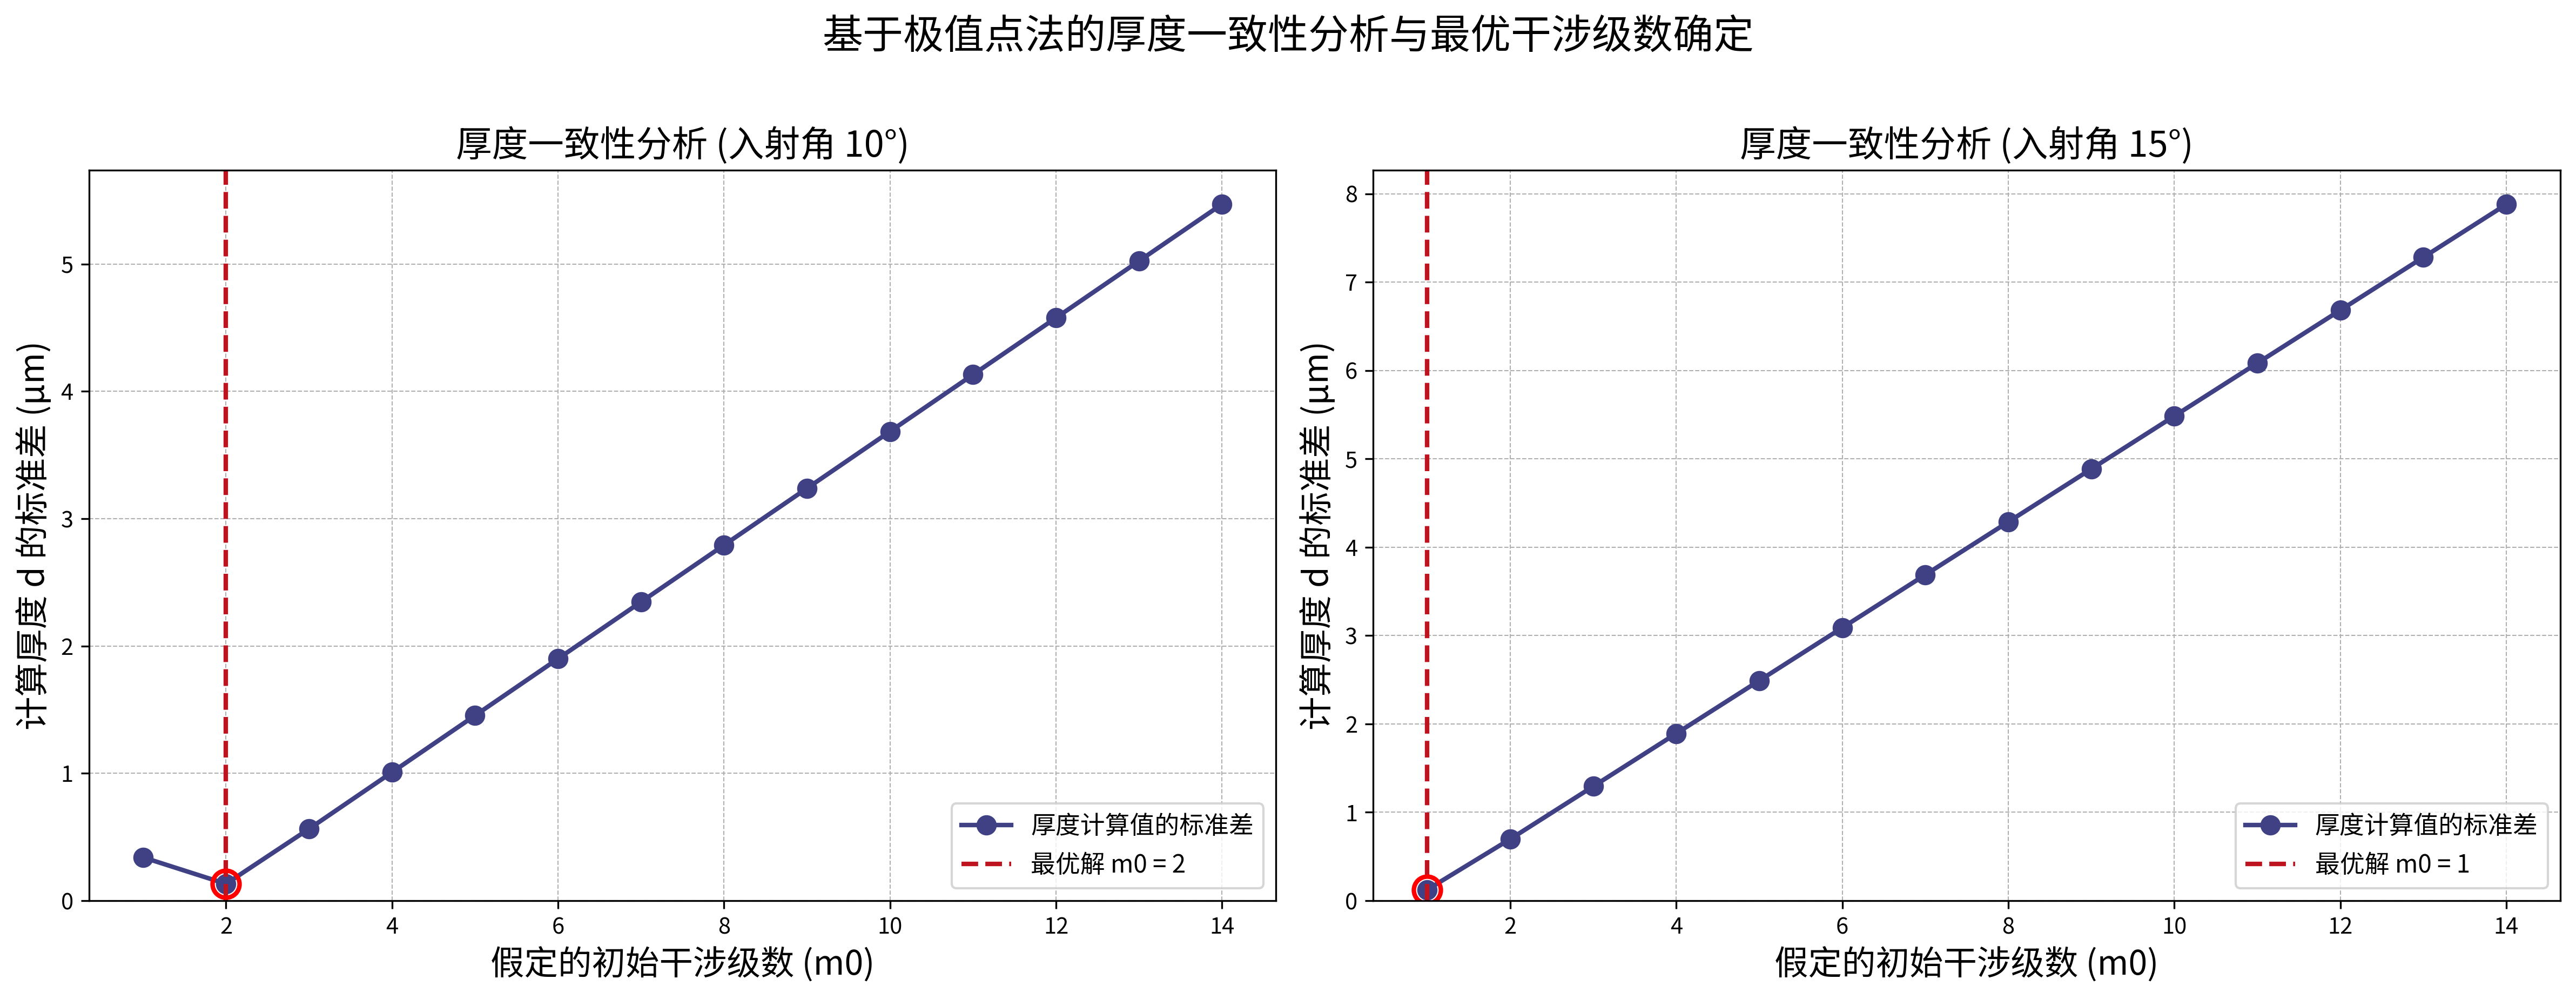
\includegraphics[width=\textwidth]{厚度一致性分析_组合图.png}
  \caption{干涉极值法得出的厚度一致性与最优干涉级数确定图}
  \label{fig:干涉极值}
\end{figure}
干涉极值法得出的结果如图（\ref{fig:干涉极值}），对于附件3，算法在初始干涉级数 $m_0=2$ 时取得最小标准差，计算得到的外延层厚度为 $\mathbf{d_3 = 3.7504 \, \mu m}$。对于附件4，算法在初始干涉级数 $m_0=1$ 时取得最小标准差，计算得到的外延层厚度为 $\mathbf{d_4 = 3.7520 \, \mu m}$，相对误差约为 $0.04\%$，可判断最终结果约为$\mathbf{d = 3.75 \, \mu m}$。

\subsection{测试结果发生多光束干涉的证明}
\subsubsection{相干性条件与几何均匀性条件：}

反射率函数有显著的波动性，利用多光束波动模型计算得到的结果稳定高，且图像形貌满足多光束干涉现象，判断满足相干性条件和几何均匀性条件。

\subsubsection{反射率与吸收条件：}

在计算得到外延层厚度后，可通过反射率实验数值与菲涅尔公式，反解出$n_2$随波数的变化关系图。将$n_2$的结果反带回菲涅尔公式，可以算出直接反射光相对振幅大小$|\tilde{U_1}|$、经过透射后一次反射光$|\tilde{U_2}|$等，据此作出前五个反射光相对振幅大小随波数变化图：
\begin{figure}[h]
  \centering
  % 指定图片文件，png/jpg/pdf 都可以
  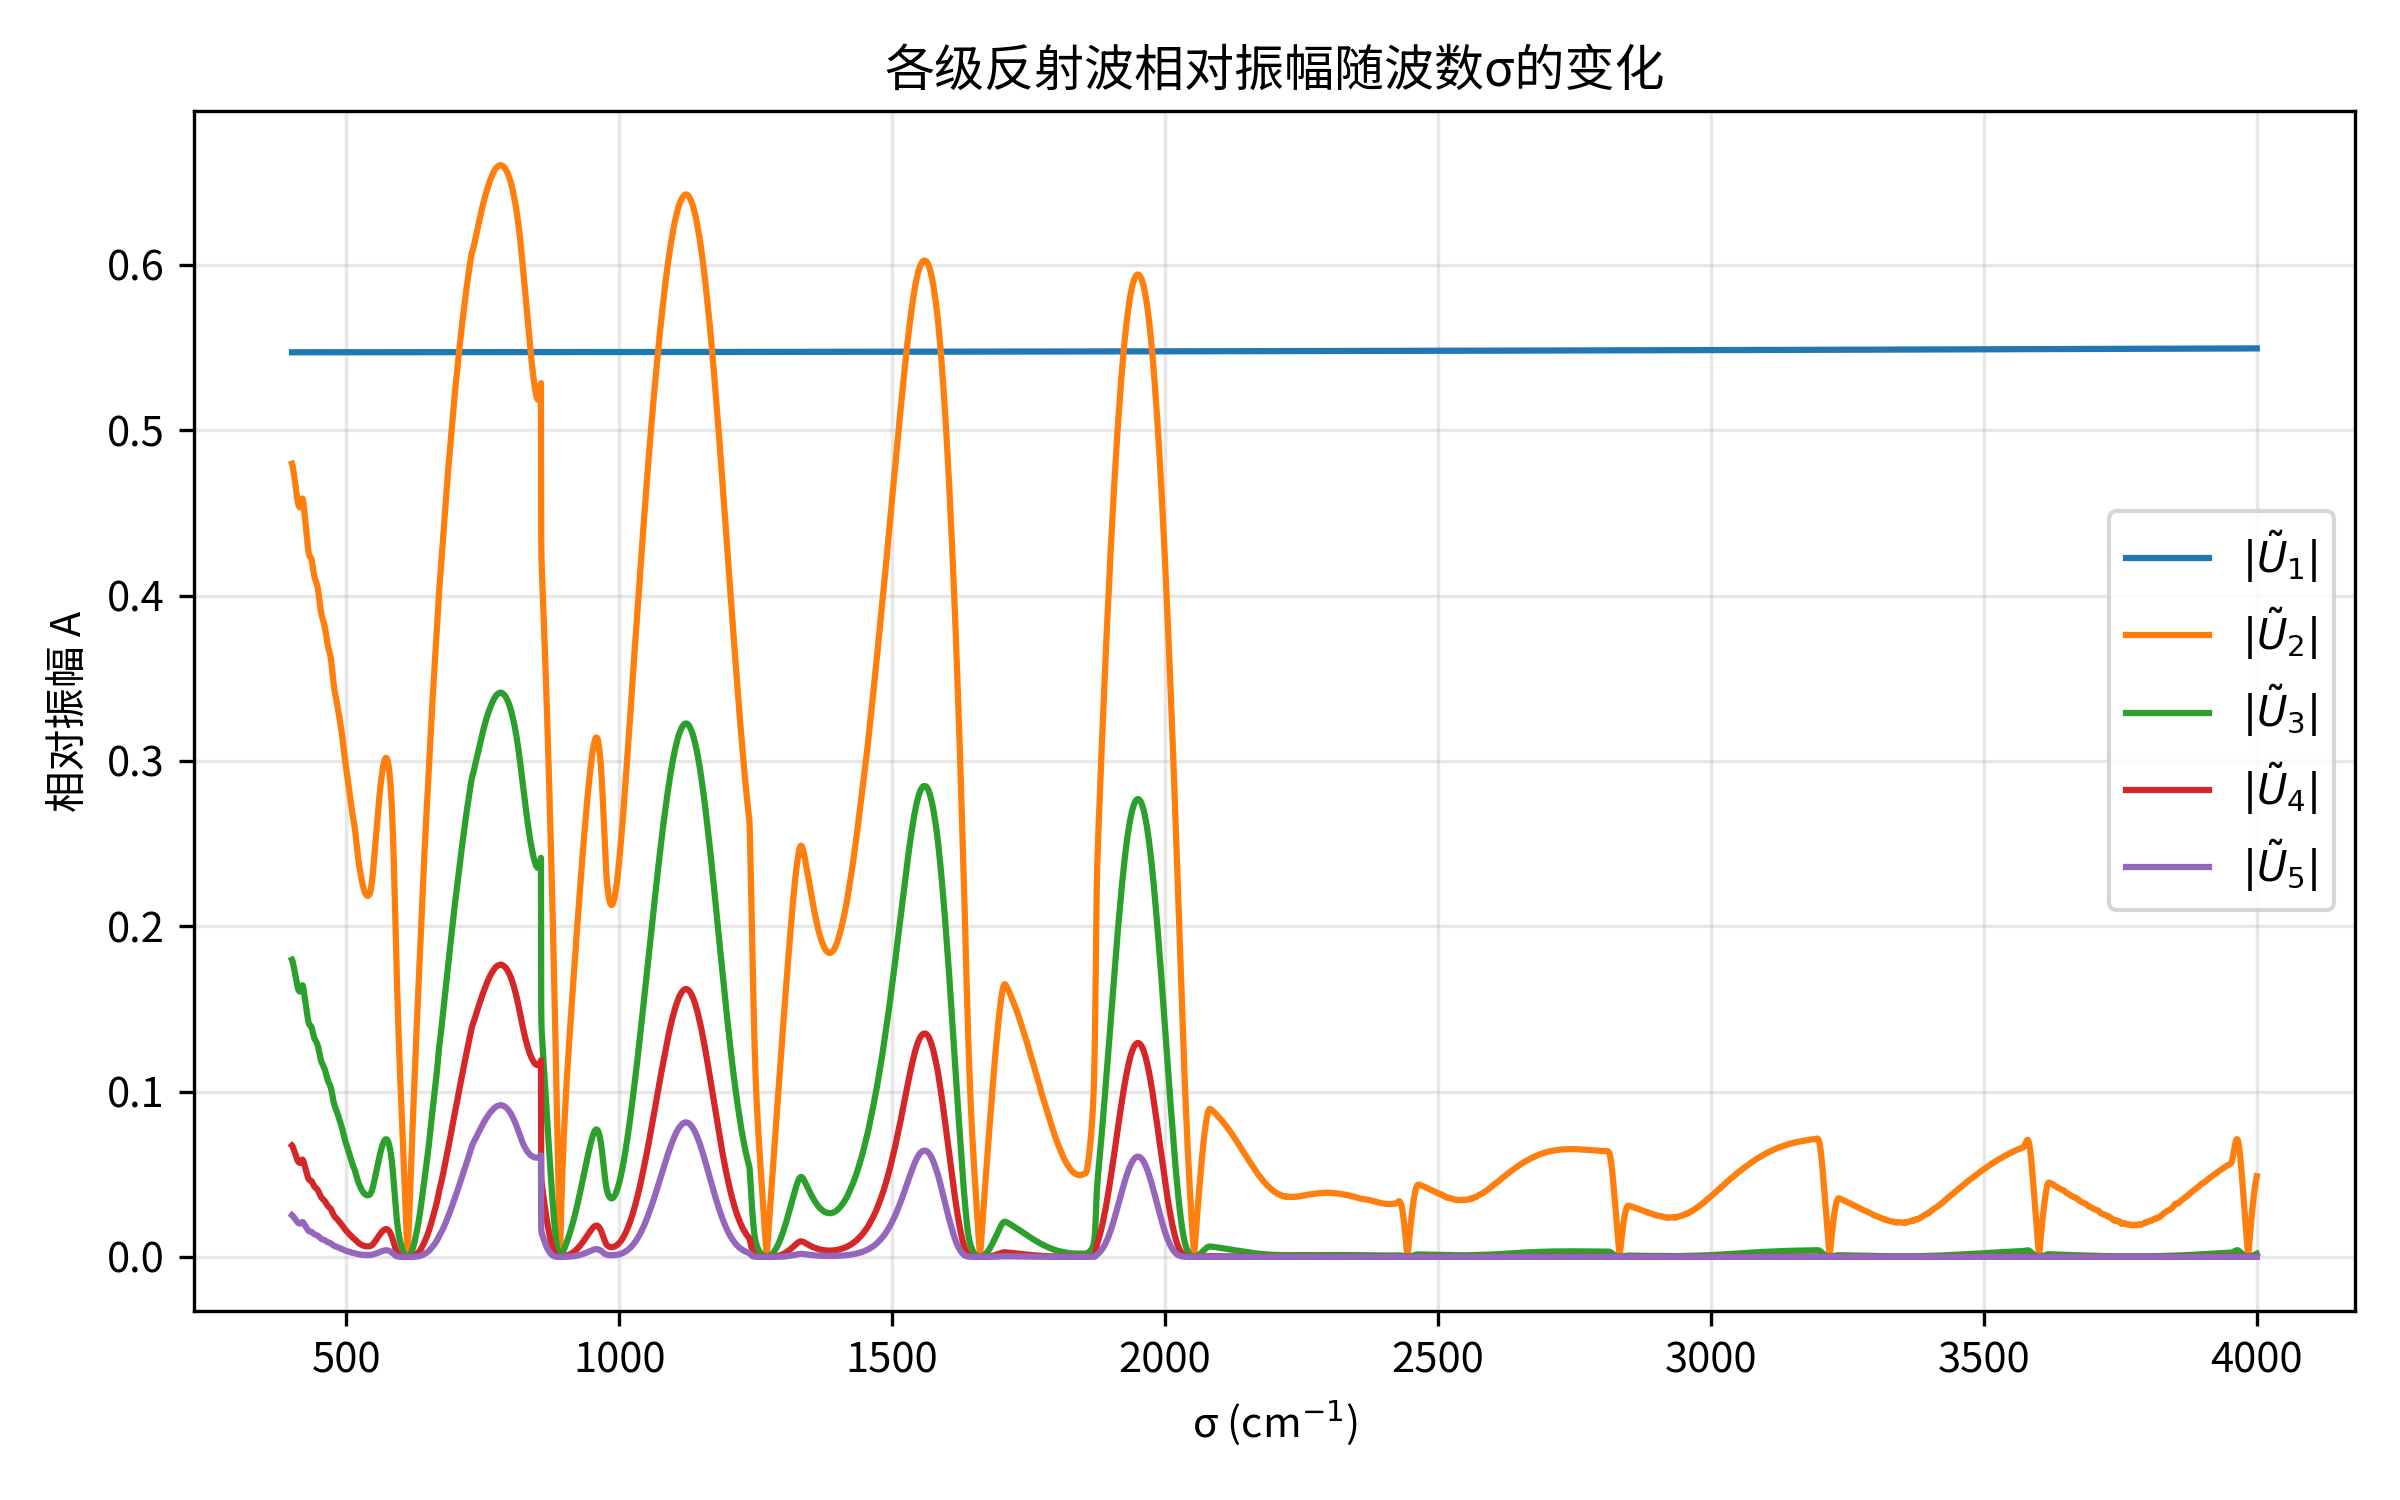
\includegraphics[width=\textwidth]{多级反射光.png}
  \caption{各级反射光相对光强随波数变化图像}
  \label{fig:干涉}
\end{figure}

根据图像可以发现，在波数位于400-2000$cm^{-1}$区间，各级反射光光振幅较大，多光束干涉效应明显,经过估算得到：
\begin{equation}
    \left|\frac{\tilde{U}_{k+1}}{\tilde{U}_k}\right| = \left|r_1'r_2e^{-i\delta} \right| \approx 0.5
\end{equation}
满足发生多光束干涉的判定条件。

\subsubsection{精细度判定条件:}

将数据代入公式（\ref{fitness}）计算，附件3、4的实验光谱对应的精细度分别为2.7079和2.6740，大于2，由此可判断硅晶圆片产生了多光束干涉。



\subsection{基于色散矫正的傅里叶变换的外延层厚度数学模型}

在对数据的处理过程中，我们发现存在信噪比较低和干涉条纹不清晰的现象。并由图13观察发现，当波数大于2000$cm^{-1}$时，经过多级反射的光振幅明显减弱，多光束干涉效应不再明显，导致难以准确定位极值点。

为了充分利用实验数据，我们和AI\cite{ai:claude}讨论并引入了基于快速傅里叶变换（FFT）的分析方法来从信号中提取频率信息，计算出外延层厚度。其中，我们创新性地通过坐标变换解决了硅的色散导致干涉信号在波数域内并非严格周期性的问题。


\subsubsection{算法核心思想与色散问题}
我们首先回顾干涉的相位差公式：
\begin{equation}
    \delta(\sigma) = 4\pi d \cdot \sigma \cdot n_f(\sigma)cos(\theta_j)
\end{equation}
其中，$\sigma$是波数，$d$是外延层厚度，$n_f(\sigma)$是外延层随波数变化的折射率，$\theta_i$是光在空气中的入射角,$\theta_j$是光在外延层中的折射角。

利用斯涅尔公式，并考虑到本问折射率为实数：
\begin{equation}
    \delta(\sigma) = 4\pi d \cdot \sigma \cdot \sqrt{n_f(\sigma)^2 - \sin^2(\theta_i)}
\end{equation}

若直接对以波数$\sigma$为自变量的反射光谱进行傅里叶变换，会遇到问题：由于折射率$n_f(\sigma)$的存在，相位差$\delta$与波数$\sigma$之间并非严格的线性关系。这意味着直接对其进行FFT会导致频谱中的峰变宽并产生位置偏移，从而引入系统误差。

\subsubsection{坐标变换：线性化相位}
为了解决此问题，我们决定在进行FFT之前，对数据进行一次坐标变换，将其从波数域转换到一个新的坐标域，在这个新域里，干涉信号具有周期性。根据相位公式，我们定义一个新的坐标变量$x$：
\begin{equation}
    x(\sigma) = 2 \sigma \sqrt{n_f(\sigma)^2 - \sin^2(\theta_i)}
    \label{eq:coord_transform}
\end{equation}
将此新坐标代入相位公式，我们得到：
\begin{equation}
    \delta(x) = 2\pi d \cdot x
\end{equation}
在这个新的$x$域中，相位差与坐标$x$呈现较好的线性关系，所以反射光谱$R(x)$是一个真正意义上的周期信号，通过对信号进行建模分析可以计算得到厚度$d$。

\subsubsection{算法流程}
我们和AI\cite{ai:gemini}优化了算法细节，如增加了汉宁窗函数的应用。最终算法流程如下：

\begin{enumerate}
    \item \textbf{数据预处理与坐标变换}: 
    我们手动标记附件3、4数据的波峰波谷位置$(\sigma_i, R_i)$，利用公式（\ref{eq:coord_transform}）和公式（\ref{eq:sellmeier_si_3term}），计算出每个原始波数点$\sigma_i$所对应的非均匀坐标点$x_i$。为了进行FFT，我们必须将光谱数据转化为具有周期性的函数，因此我们通过线性插值法，将反射率数据$R$重新采样到一个均匀间隔的新坐标网格$x_{uniform}$上。为提高分辨率，我们选取16384为采样点数。

    \item \textbf{窗函数应用}: 
    由于我们处理的是有限长度的信号，直接进行FFT会导致信号的两端不连续，干扰主峰的识别。所以我们在FFT之前，将重采样后的信号乘了一个平滑的窗函数，我们选用汉宁窗。为使FFT频谱中的主峰更加突出，我们从信号中减去了其直流分量（均值）。

    \item \textbf{快速傅里叶变换 (FFT)}: 
    对经过加窗处理的信号应用标准的FFT算法。由于我们已经进行了精确的坐标变换，得到的FFT频谱的横坐标直接对应于薄膜的物理厚度$d$。

    \item \textbf{高精度峰定位}: 
    FFT的结果是离散的，其峰值位置被限制在频率栅格上。为了获得“亚像素”级别的精度，我们首先在FFT振幅谱中找到最大值点，然后选取该点及其左右两个相邻点，通过一个二次多项式（抛物线）进行拟合，并解析地计算出该抛物线的顶点位置。这个顶点位置就是我们最终得到的高精度厚度值。

% \begin{figure}[h!]
%   \centering
%   % 指定图片文件，png/jpg/pdf 都可以
%   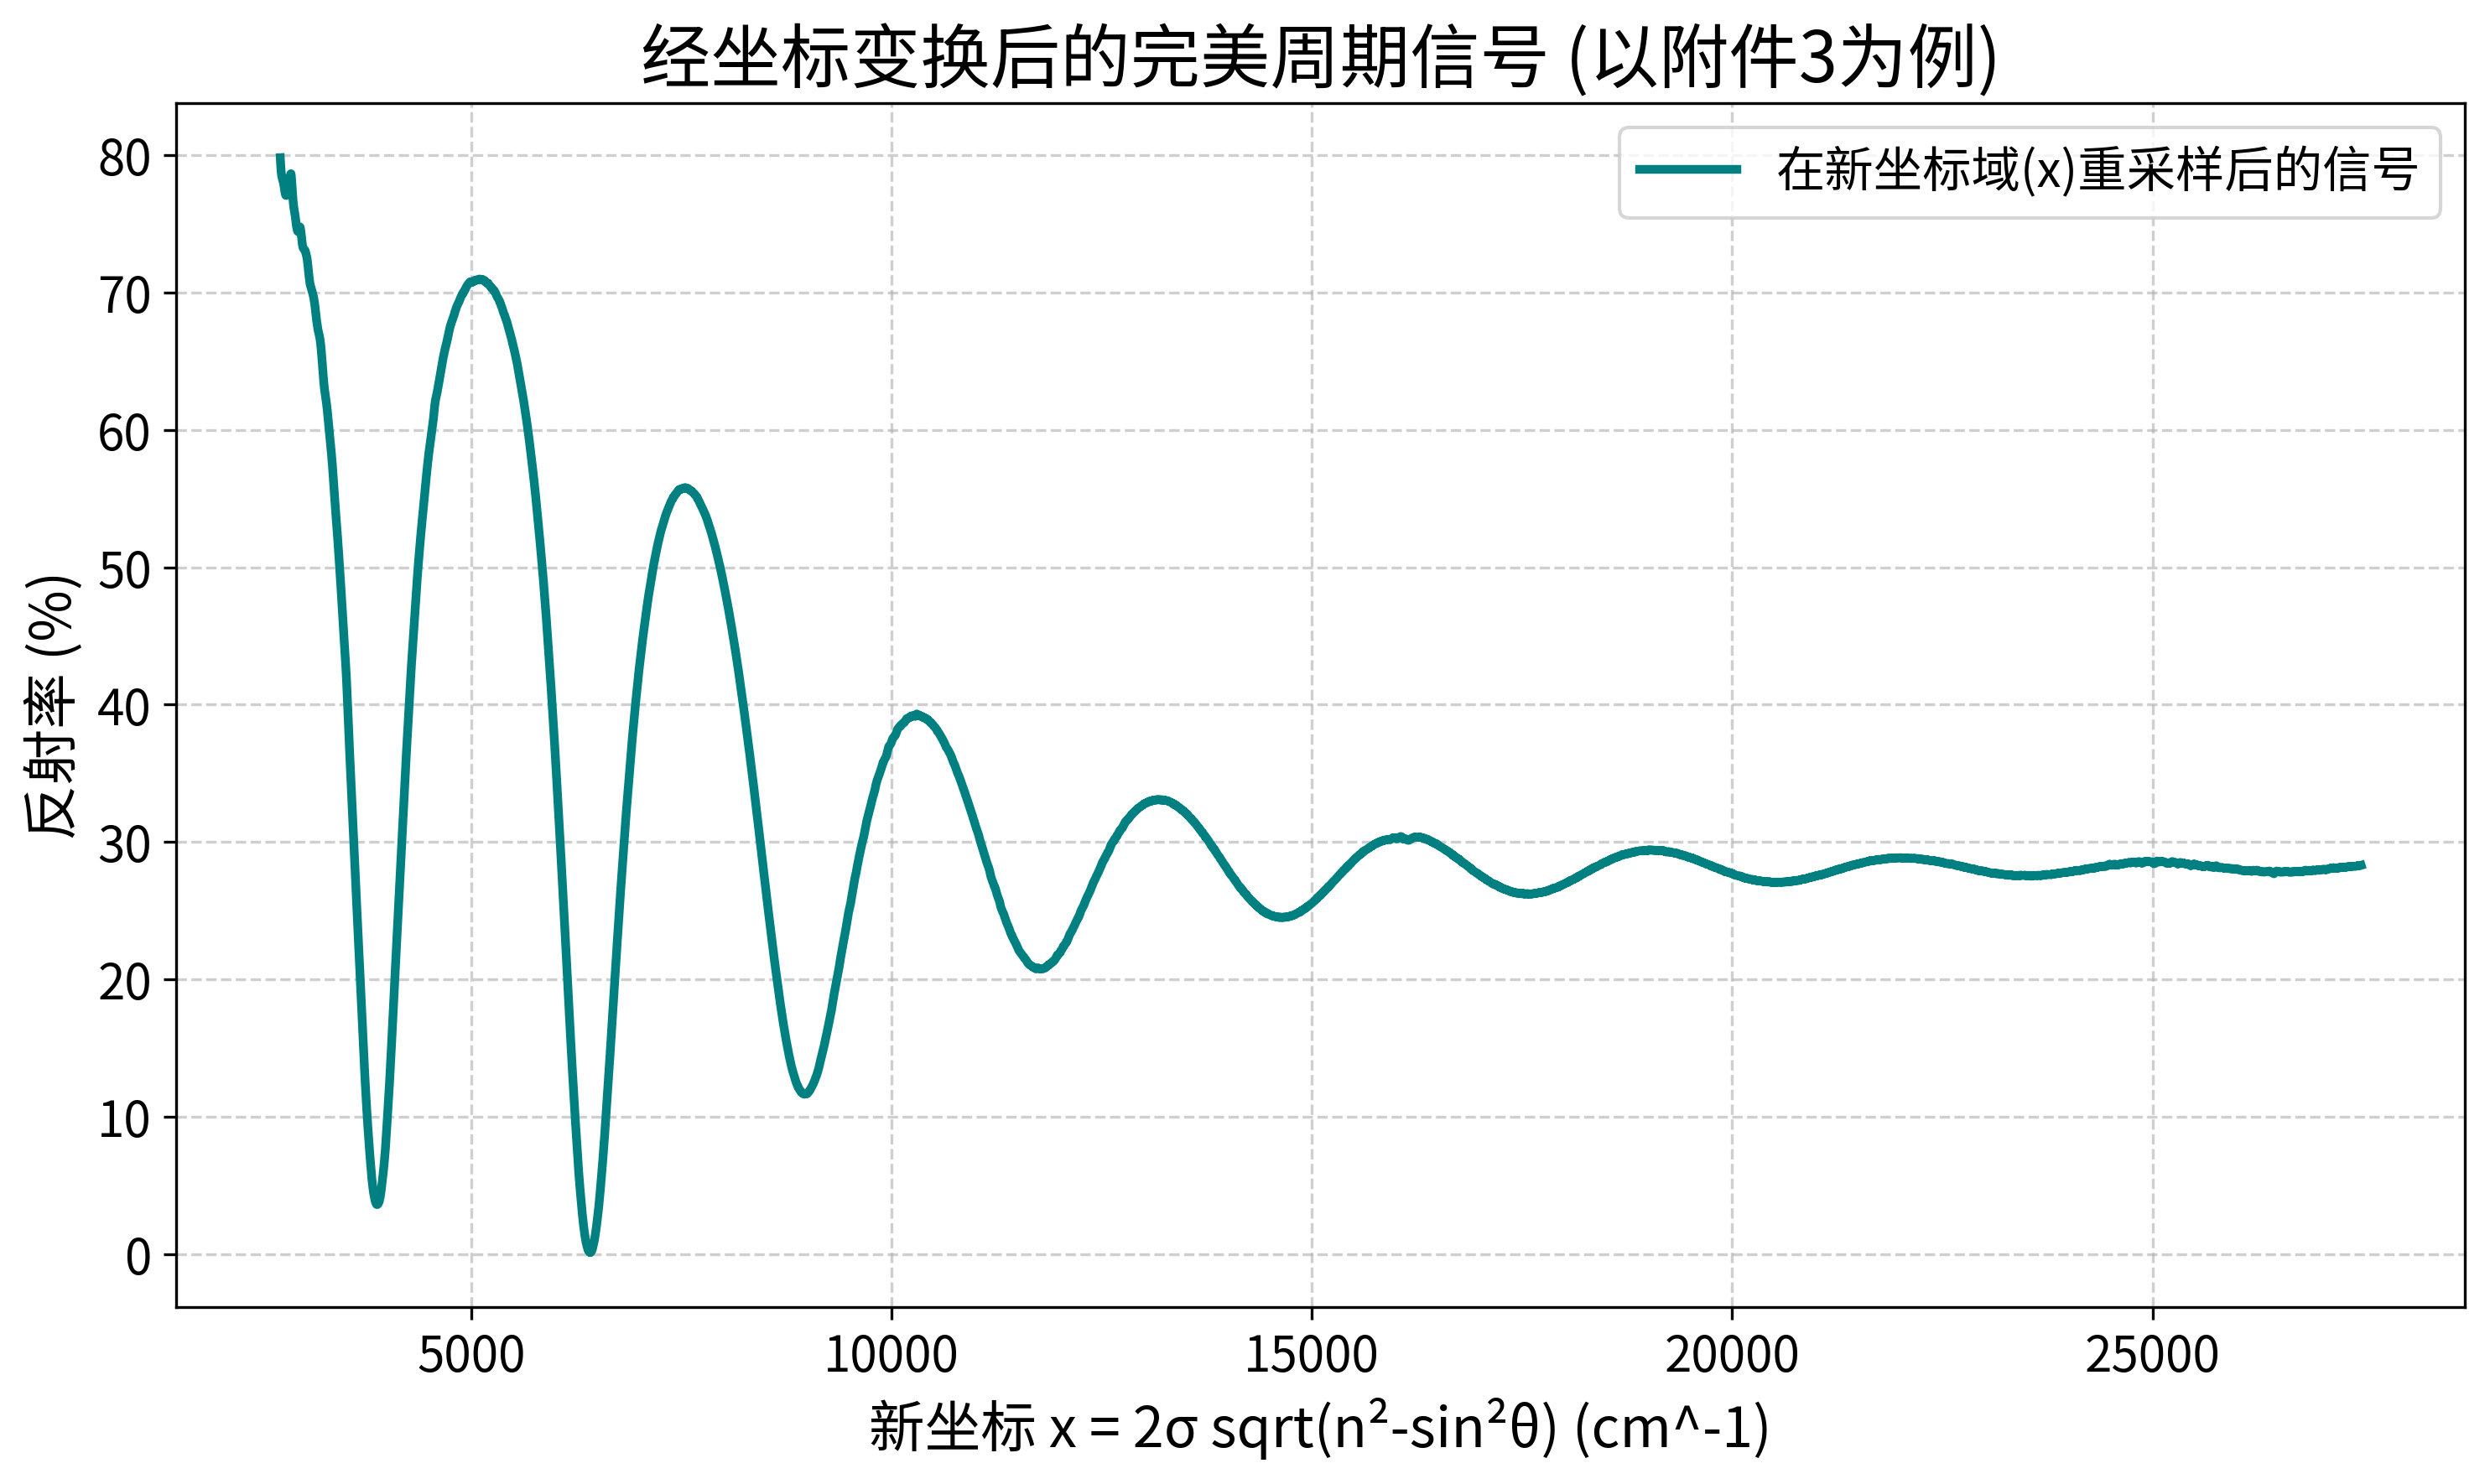
\includegraphics[width=0.75\textwidth]{信号.png}
%   \caption{}
%   \label{fig:example}
% \end{figure}
    
\end{enumerate}

\subsubsection{计算结果与交叉验证}
我们将此算法应用于附件3和附件4的数据，我们得到了相似的结果，如图（\ref{fig:fft}）。前者结果为$\mathbf{d_3 = 3.6070 \, \mu m}$，后者为$\mathbf{d_4 = 3.5833 \, \mu m}$。
% \begin{itemize}
%     \item \textbf{对于附件3 (10°)}: 算法计算出的高精度厚度为 $\mathbf{d_3 = 3.6070 \, \mu m}$。
%     \item \textbf{对于附件4 (15°)}: 算法计算出的高精度厚度为 $\mathbf{d_4 = 3.5833 \, \mu m}$。
% \end{itemize}

% \subsection{多光束干涉对外延层厚度计算精度影响}

% 多光束干涉不仅使干涉条纹呈非正弦形态，还引入了随波长变化的界面反射\textbf{相位突变}。干涉极值点法和基于傅里叶变换(FFT)的方法的结果存在约4\%的系统性差异，我们认为其根源在于两种算法对多光束干涉物理效应的敏感度不同。

% \textbf{干涉极值点法}对极值点的绝对位置敏感，而未被模型完全描述的相位突变会给这些位置带来微小但系统的偏移，从而引入系统误差。\textbf{基于傅里叶变换(FFT)的方法}则展现出更强的鲁棒性。它分析的是整个信号的\textbf{主导振荡频率}。面对非正弦信号，它能准确锁定基频；面对缓慢变化的相位扰动，它通过对全谱积分变换有效地“平均掉”了这些影响。

% 基于傅里叶变换的方法因其对全局频率特性的分析本质，能更好地抵抗这些扰动，因此我们认为其计算结果精度更高。

\subsection{外延层厚度最终结论}
经过以上对计算精度的分析，我们最终选择基于傅里叶变换(FFT)的方法求解出来的结果，也就是对于附件3 (10°)，厚度为$\mathbf{d_3 = 3.6070 \, \mu m}$。对于附件4 (15°)，厚度为$\mathbf{d_4 = 3.5833 \, \mu m}$，结果在误差范围内，我们取两次计算结果的平均值\textbf{3.5952 μm}作为最终报告厚度。
\begin{figure}[H]
  \centering
  % 指定图片文件，png/jpg/pdf 都可以
  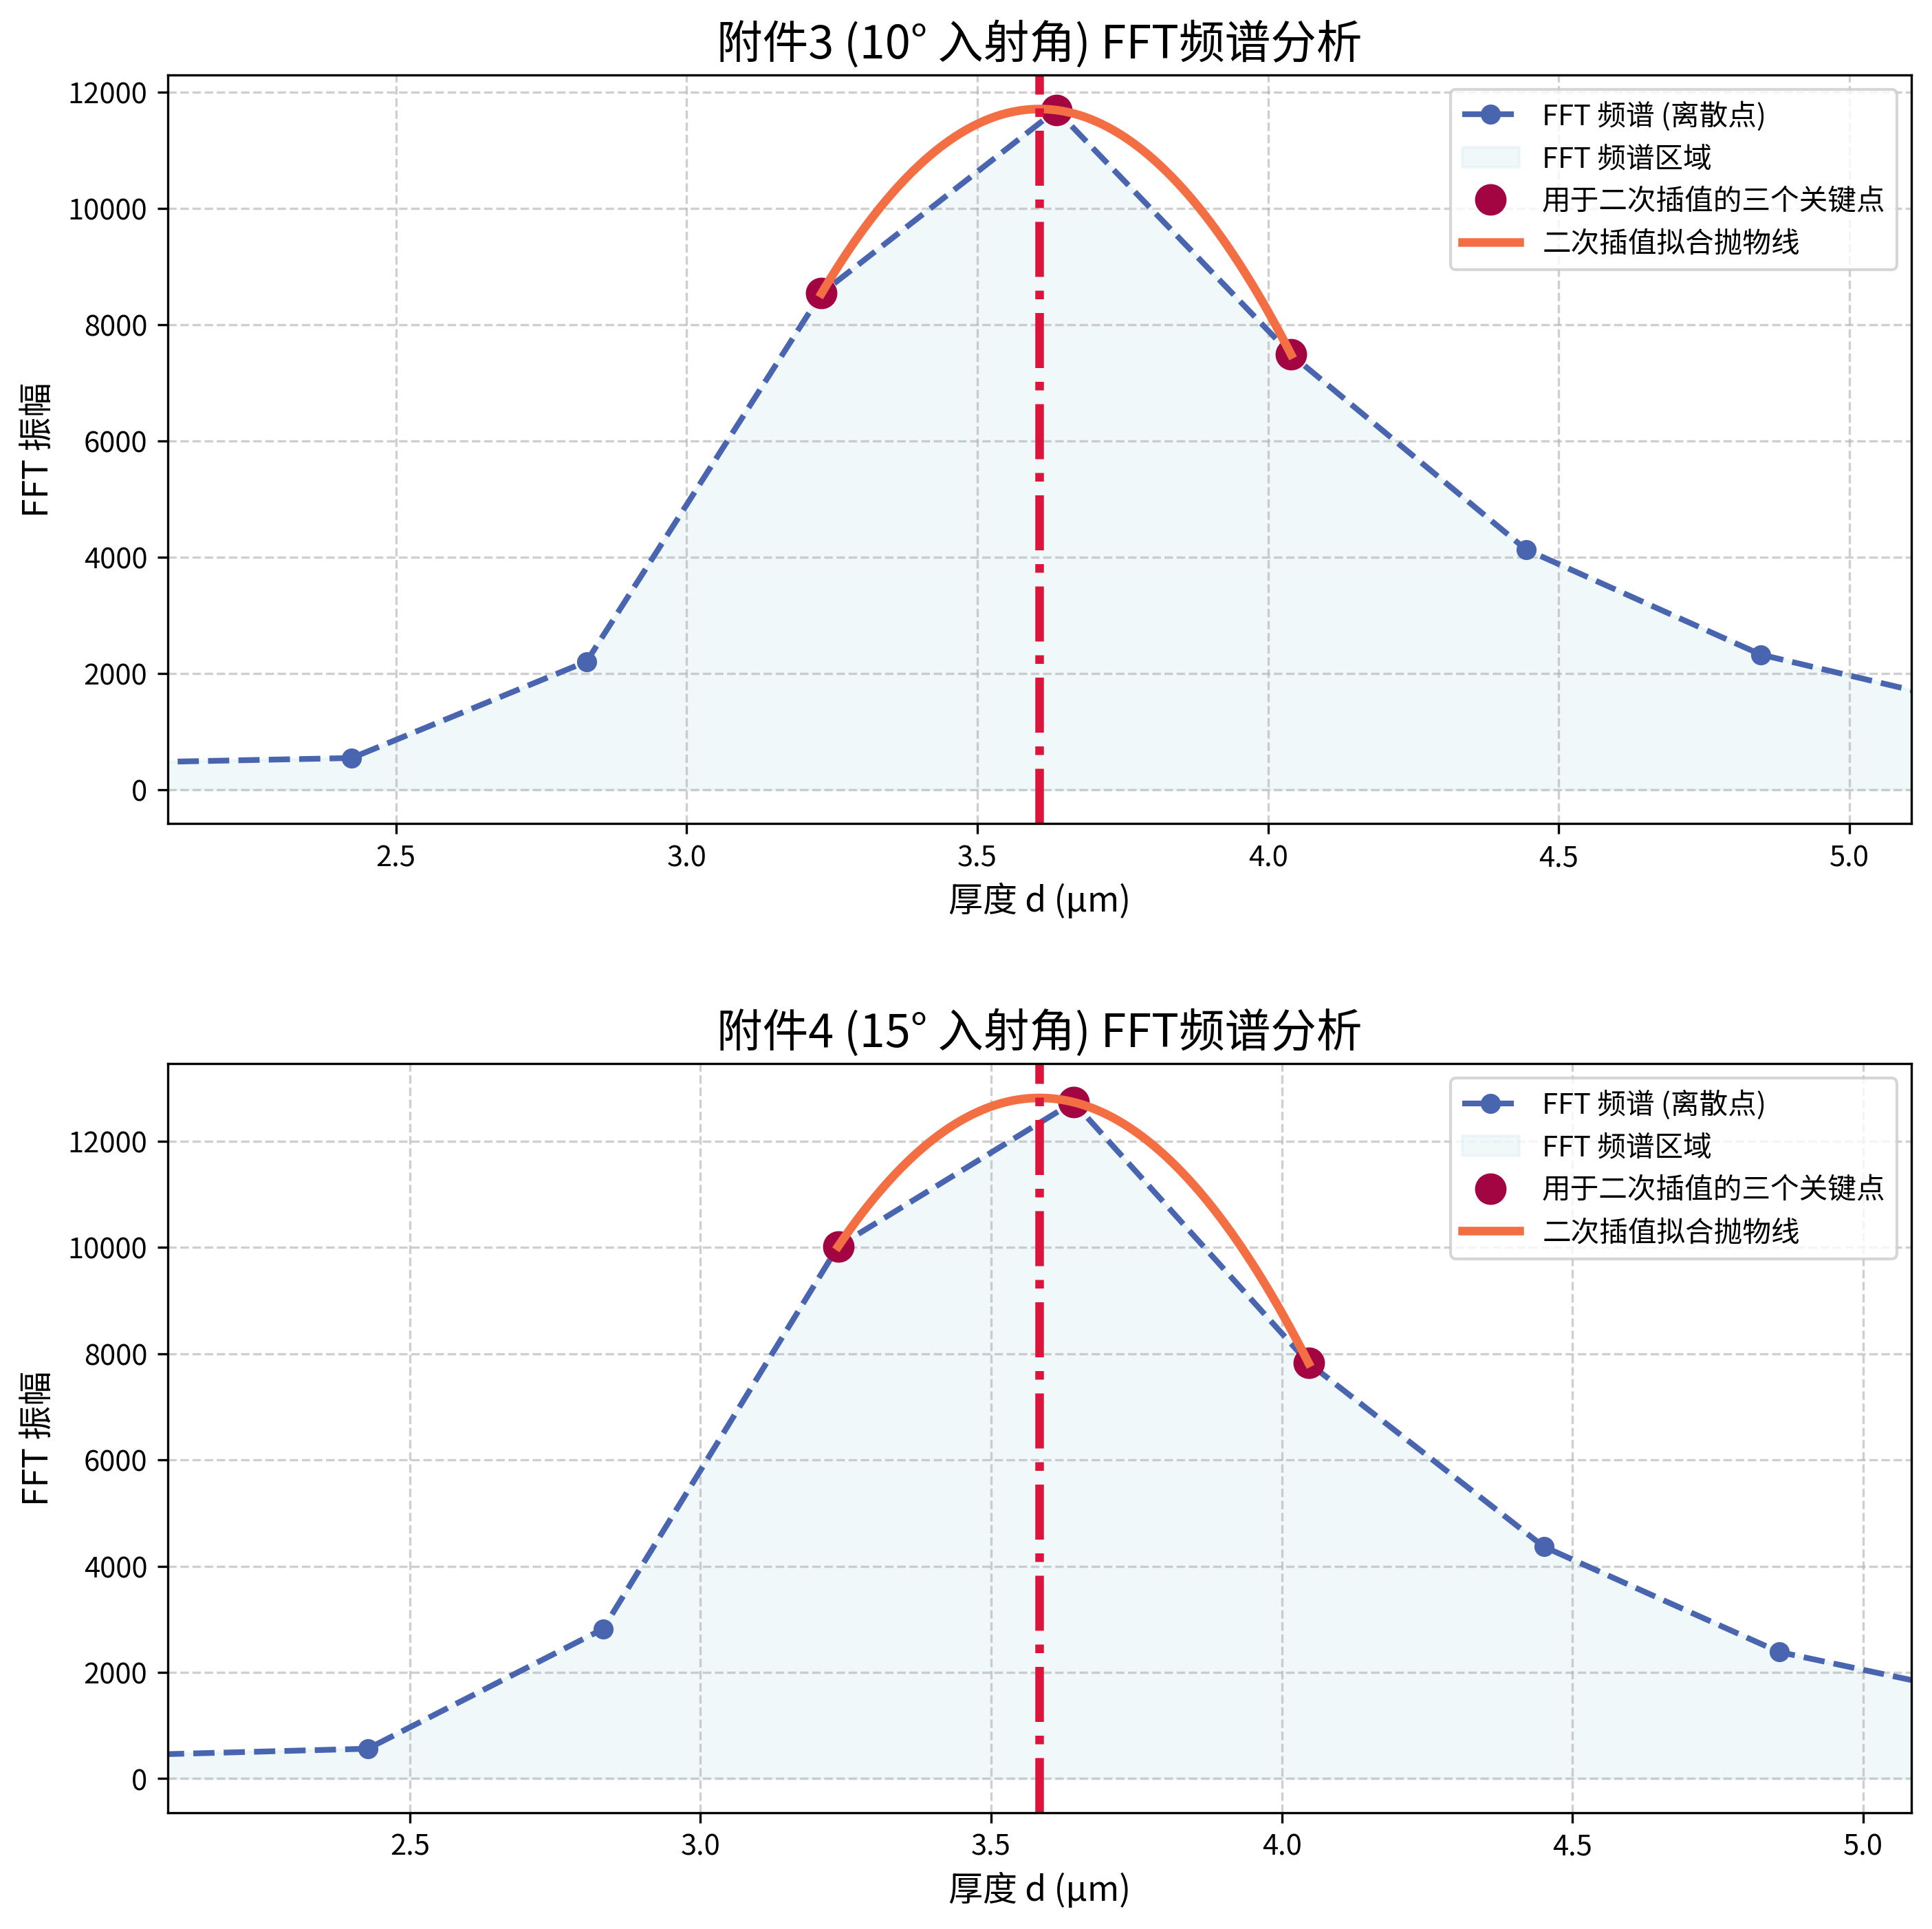
\includegraphics[width=0.65\textwidth]{fft.png}
  \caption{对于入射角10°和15°的FFT频谱分析与厚度求解}
  \label{fig:fft}
\end{figure}
\section{碳化硅晶圆片的测试结果无需考虑多光束干涉的说明}
利用在处理问题二得到的折射率随波数变化图像，可以利用菲涅尔公式计算出各级反射振幅的大小，画出振幅图如图（\ref{fig:干涉}）。

\begin{figure}[H]
  \centering
  % 指定图片文件，png/jpg/pdf 都可以
  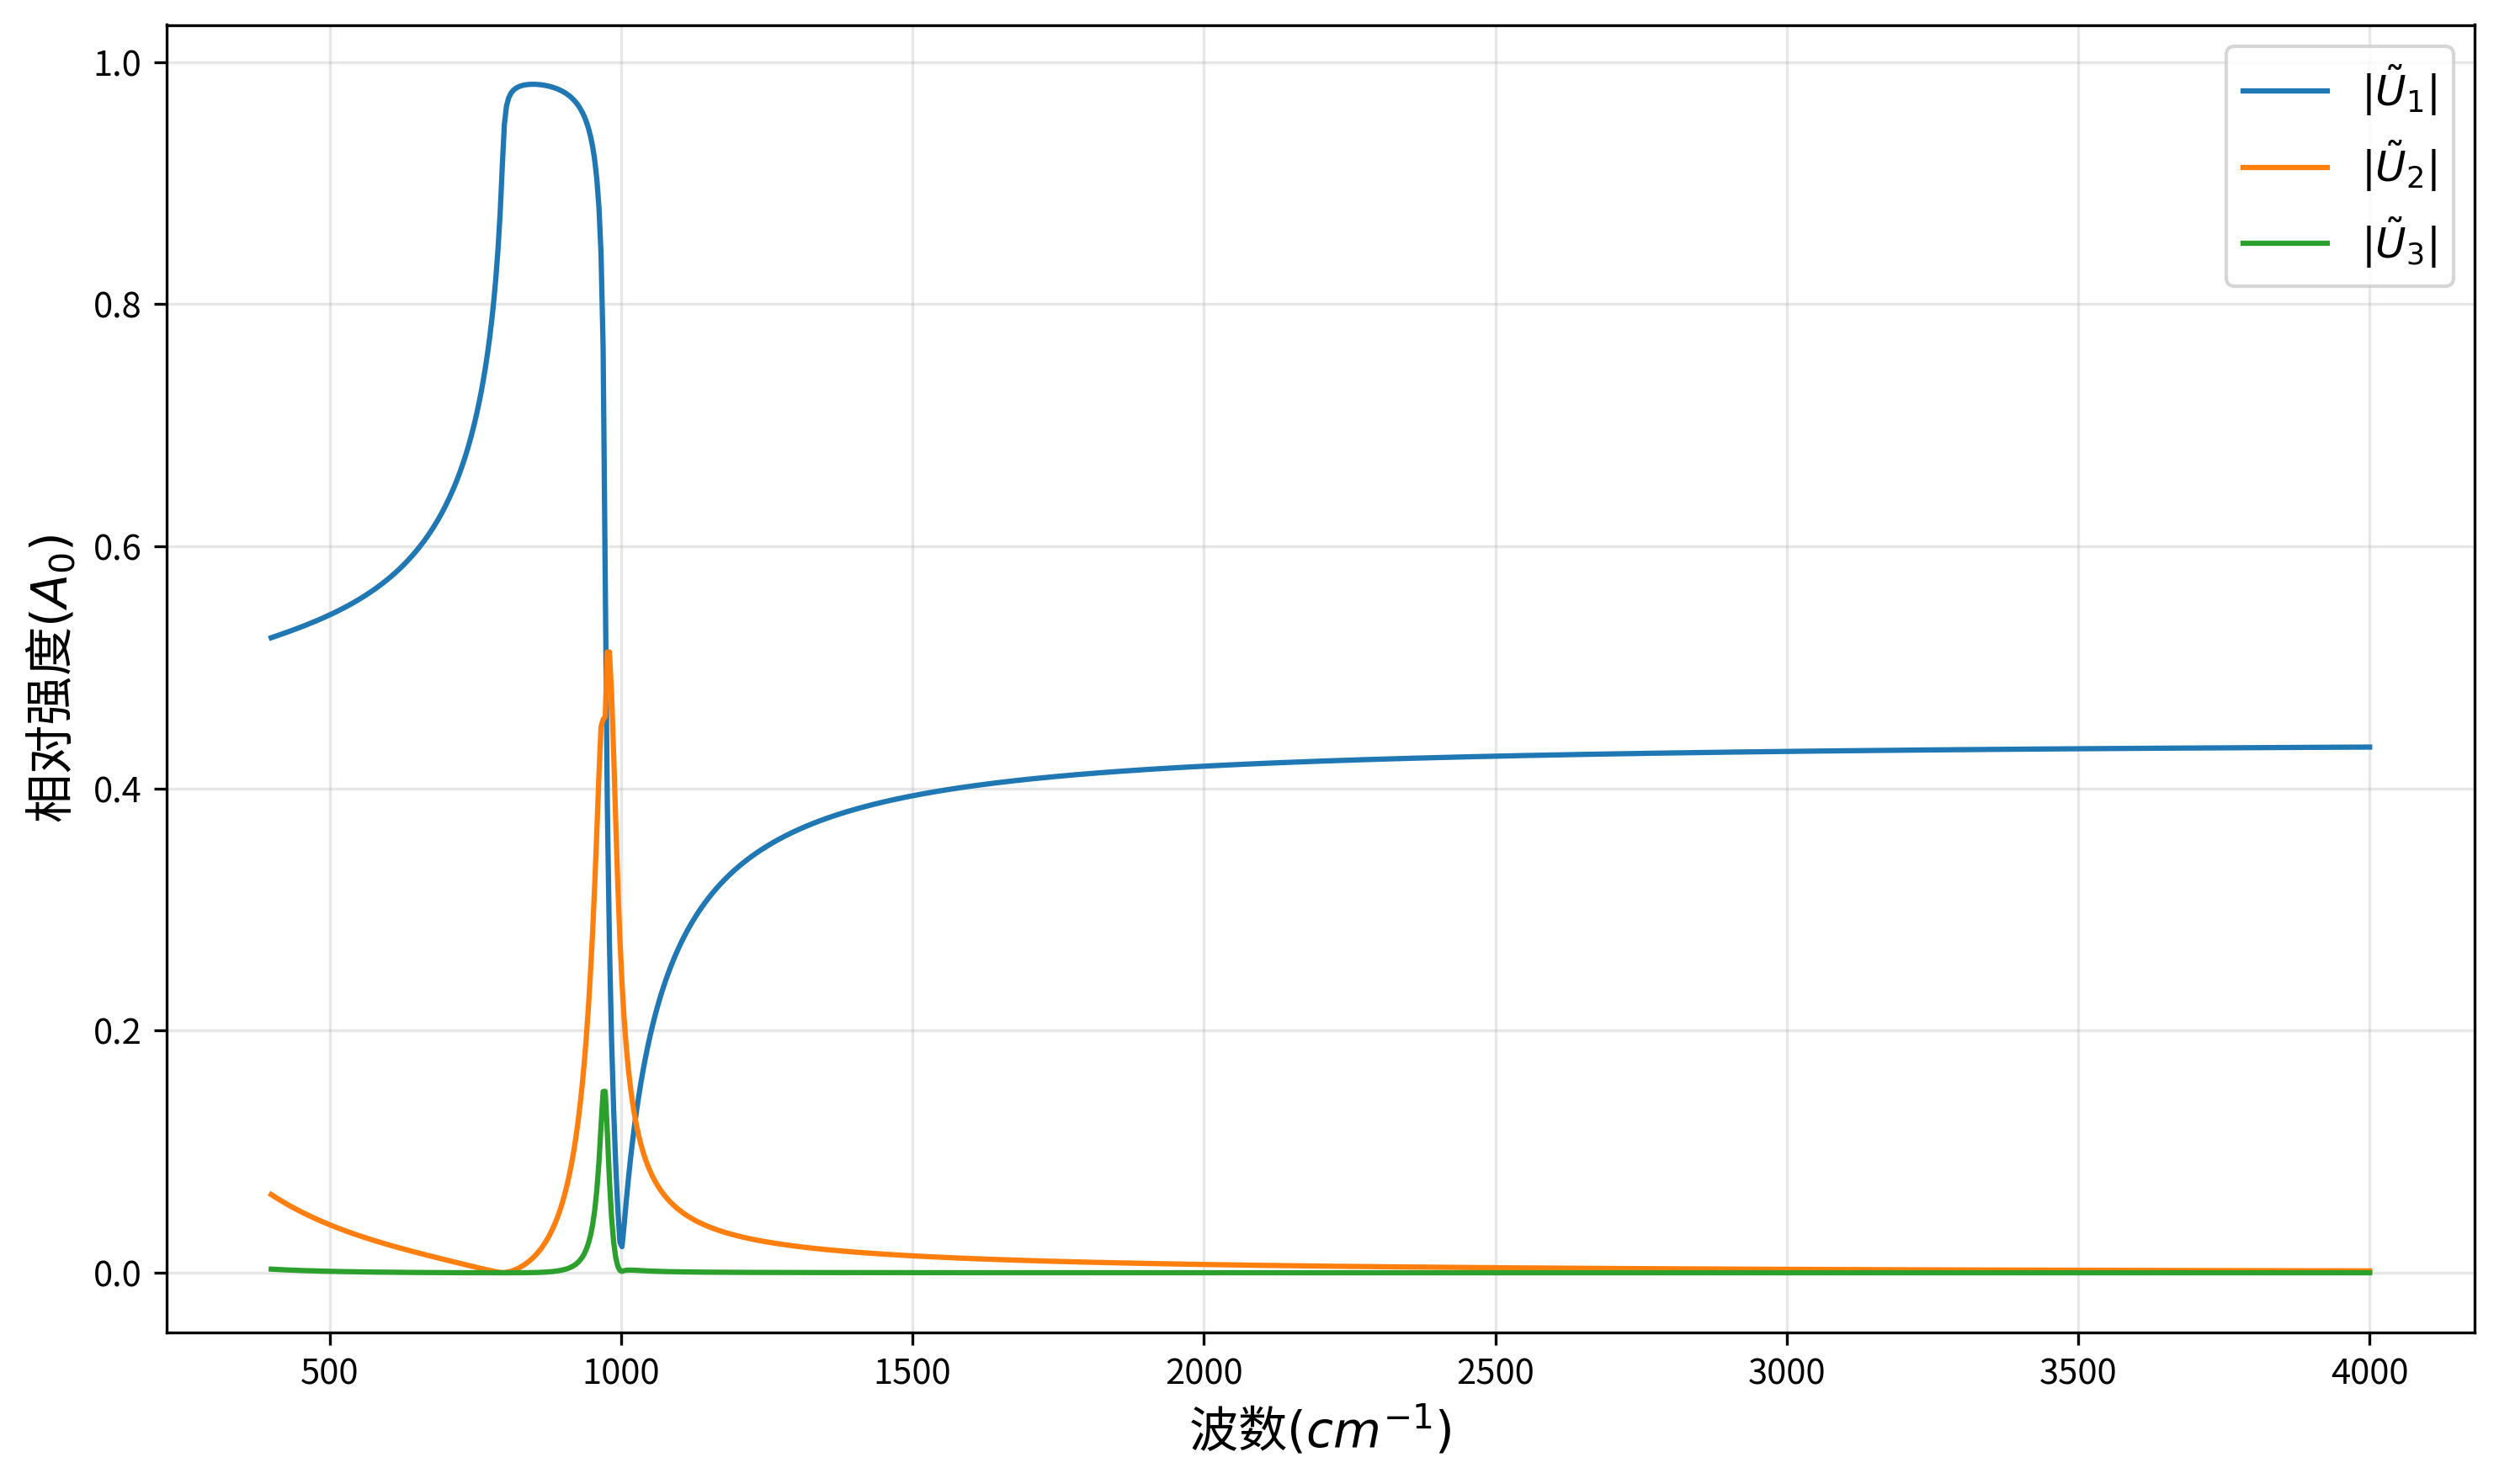
\includegraphics[width=0.65\textwidth]{双光束反射.png}
  \caption{问题二各级反射光相对强度图}
  \label{fig:干涉}
\end{figure}

根据图像，可以发现光强的主要贡献项为直接反射光。多级反射光光强远小于直接反射光和一次反射光。即：
\begin{equation}
    \left|r_1'r_2e^{-i\delta} \right| <<1
\end{equation}
所以无需考虑多光束干涉对之前计算结果的影响。


\section{模型检验}
% (1) 对模型的合理性、准确性和稳健性进行检验。
% (2) 常用的方法有：灵敏度分析、误差分析、与实际数据对比等。
\subsection{问题三基于傅里叶变换的计算外延层厚度方法灵敏度}

首先，我们分别对入射角$\theta_i$和塞尔迈耶方程中的主导色散系数$B_1$的基准值加入了$\pm2\%$和$\pm1\%$的扰动。
同时，我们还对FFT前的重采样点数\texttt{num\_points}进行了收敛性分析，以证明我们选取参数的合理性。\textbf{图（\ref{fig:sensitivity_combined}）}展示了这两项灵敏度分析的结果。

% --- 从这里开始是为您修改的并排图片代码 ---

\begin{figure}[htbp]
  \centering % 将整个图形块居中

  % --- 第一个子图 (左图) ---
  \begin{subfigure}[b]{0.49\textwidth}
    \centering
    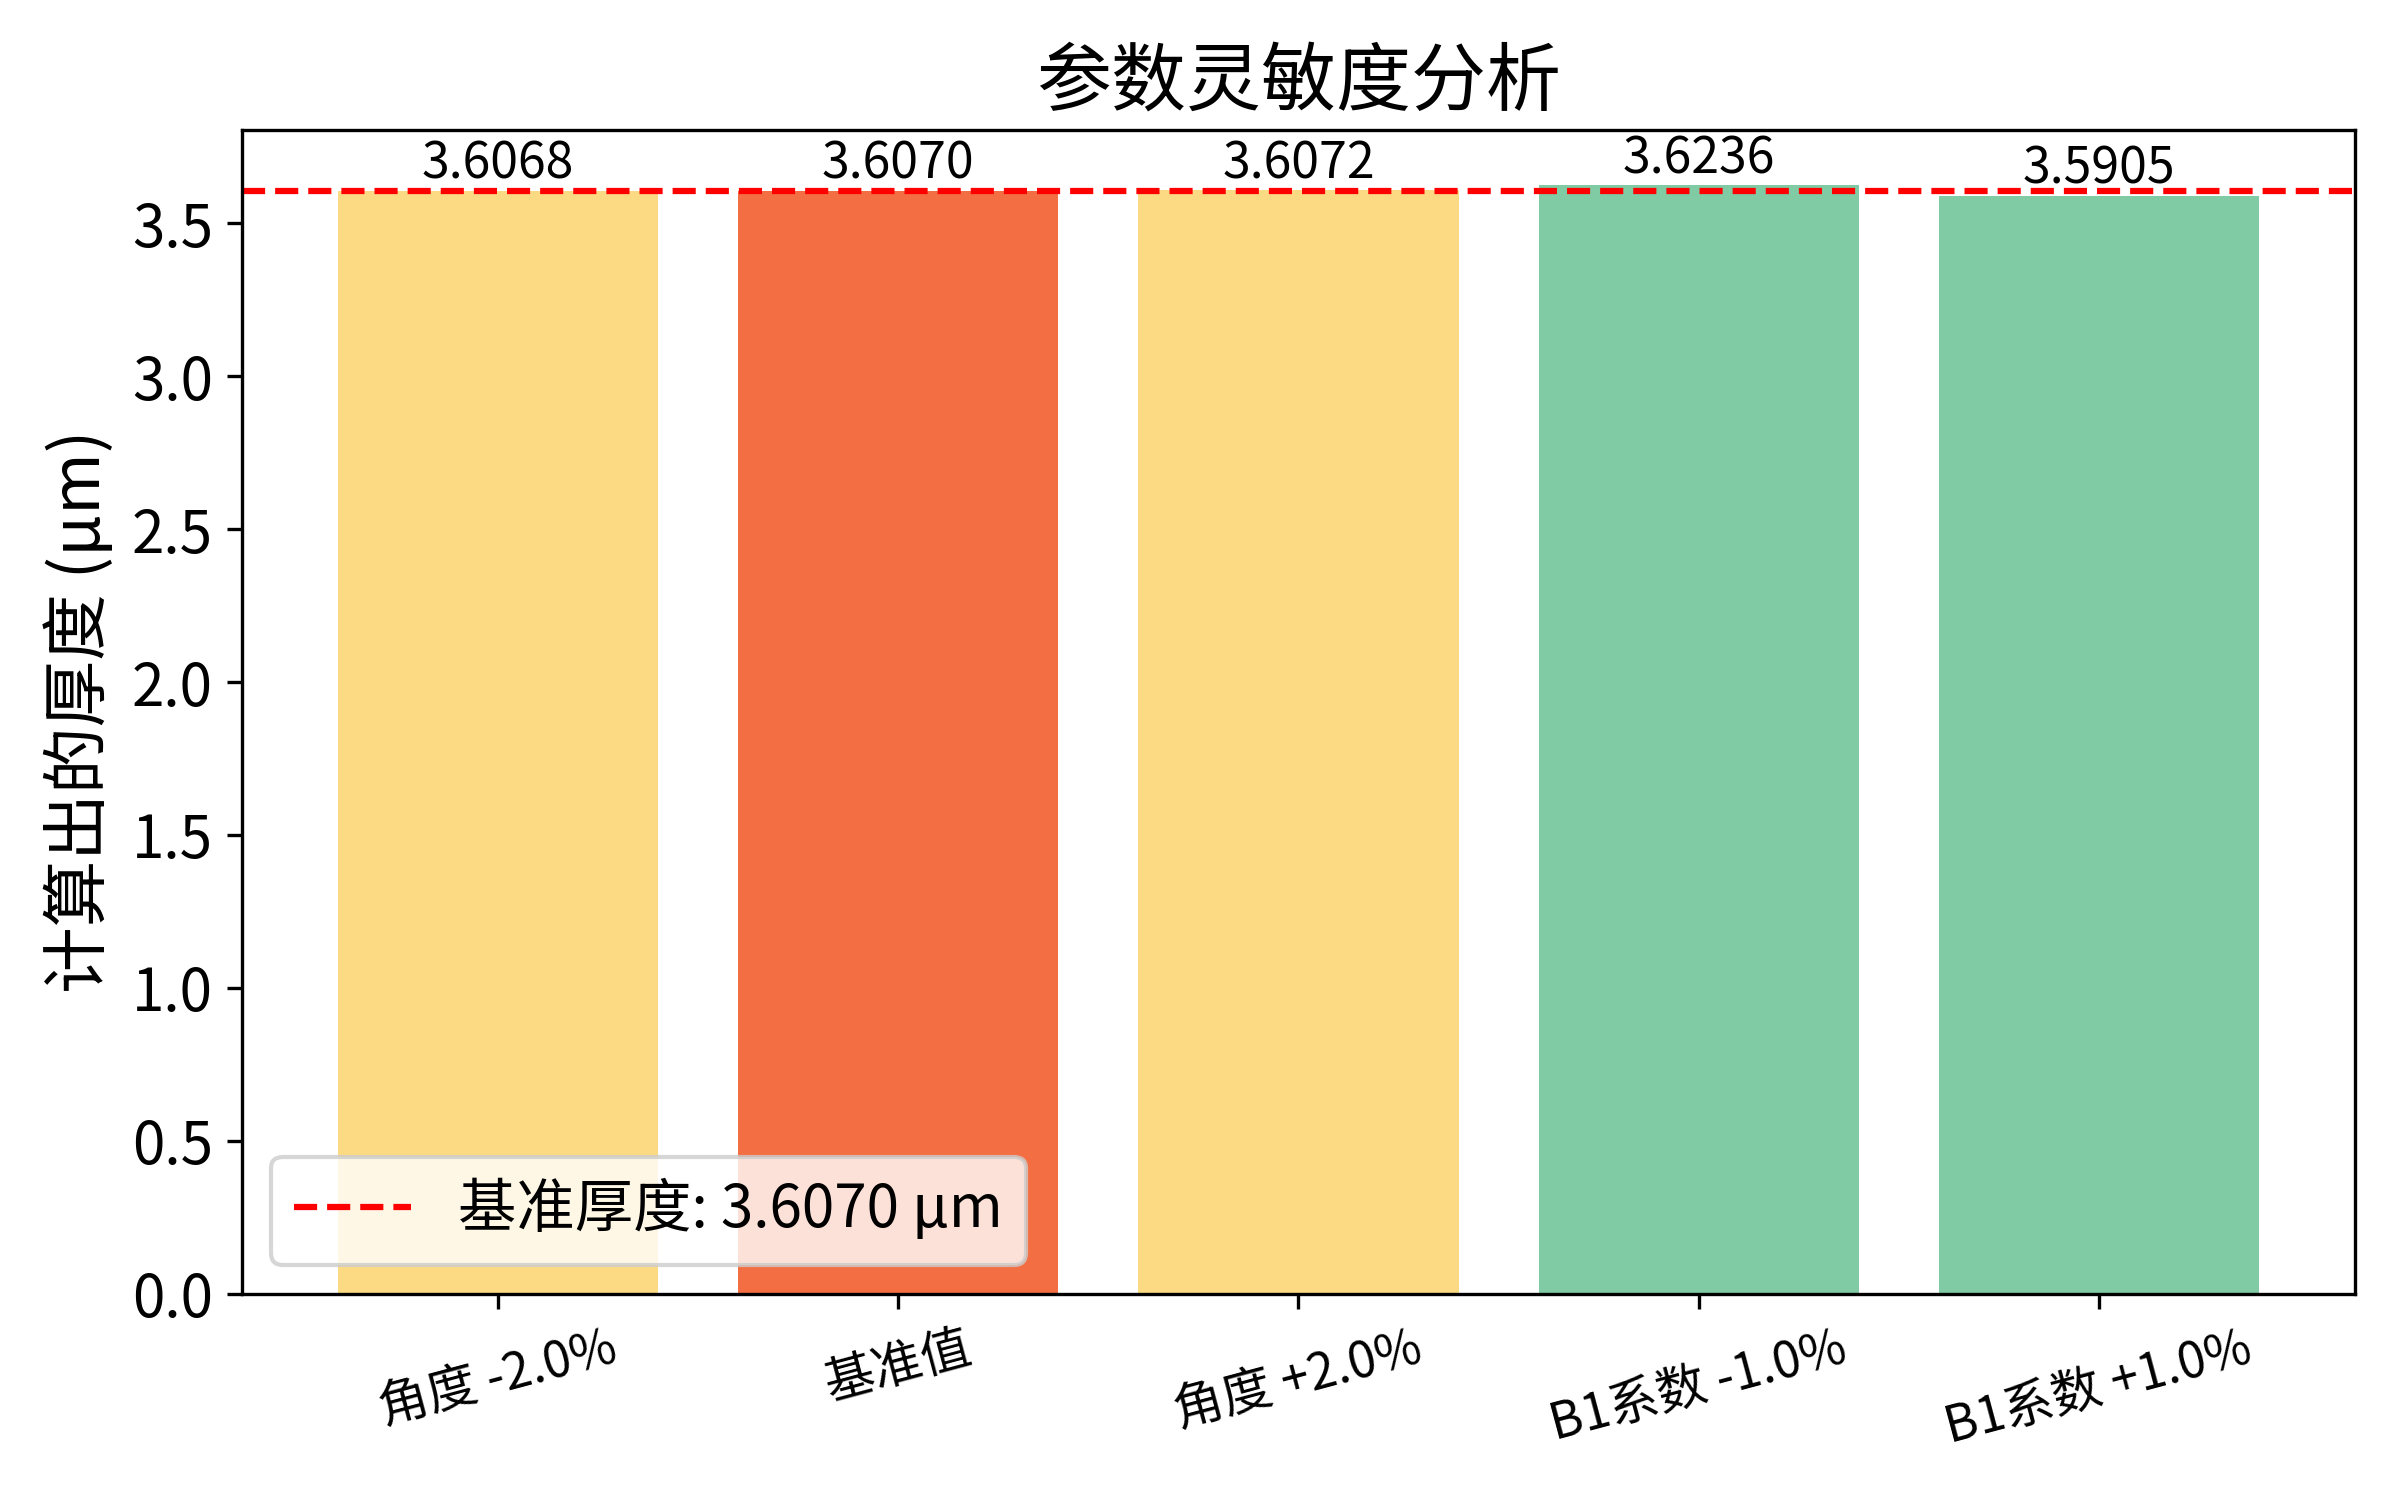
\includegraphics[width=\textwidth]{参数灵敏.png}
    \caption{模型对入射角和塞尔迈耶系数的敏感度}
    \label{fig:param_sensitivity}
  \end{subfigure}
  \hfill % 在两个子图之间添加一个弹性的水平间距
  % --- 第二个子图 (右图) ---
  \begin{subfigure}[b]{0.49\textwidth}
    \centering
    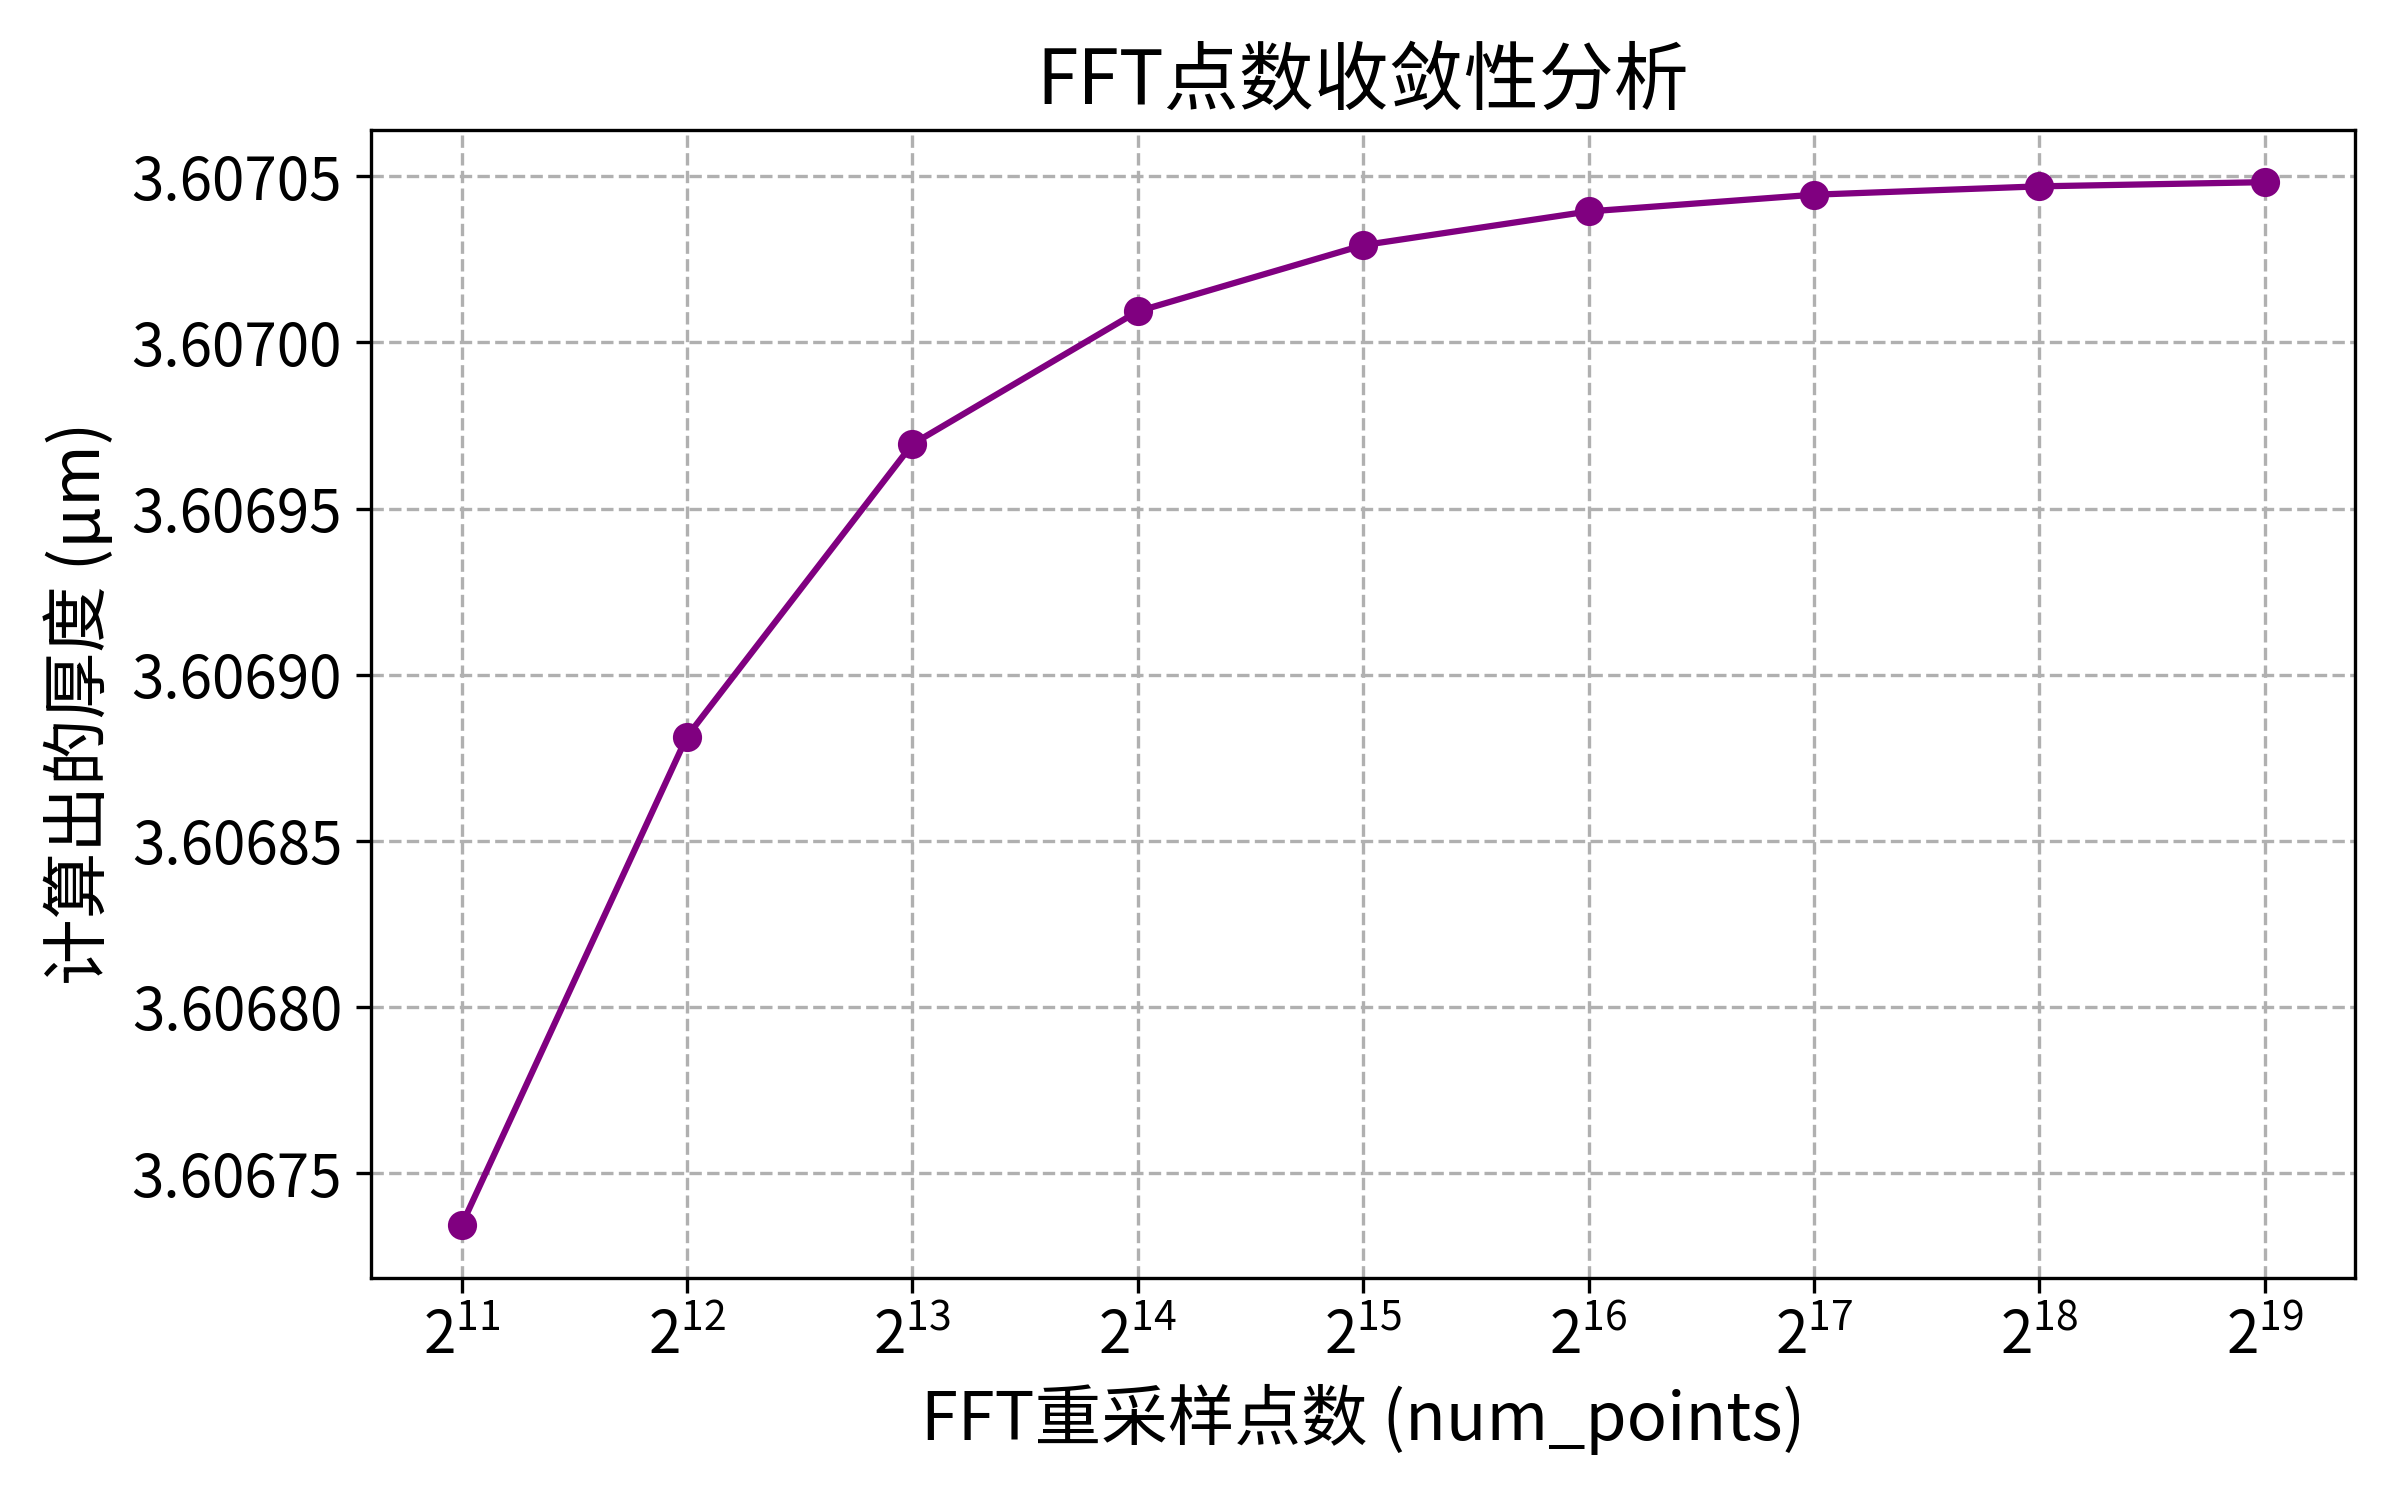
\includegraphics[width=\textwidth]{num.png}
    \caption{FFT算法关于重采样点数的收敛性}
    \label{fig:fft_convergence}
  \end{subfigure}

  % --- 整个并排图的总标题和总标签 ---
  \caption{FFT算法的灵敏度与收敛性综合分析}
  \label{fig:sensitivity_combined}
\end{figure}

从\textbf{图（\ref{fig:param_sensitivity}）}可看出，入射角仅引起厚度计算结果约0.005\%的微小波动，而$B_1$系数引起的波动也小于0.5\%。这证明了该算法在面对实际测量误差和材料光学常数不确定性时具有出色的稳健性。

同时，从\textbf{图（\ref{fig:fft_convergence}）}可以看到，当采样点数超过8192 ($2^{13}$) 时，计算结果已收敛到一个稳定的数值，进一步增加点数对结果的精度的提升已经非常小。这证明了我们在算法中所采用的点数（$2^{14}$=16384）有效。

\subsection{问题二、三外延层厚度算法稳定性检验}

\subsubsection{问题二基于双光束干涉和洛伦兹-德鲁德模型计算外延层厚度方法稳定性}
我们对附件1和2的原始反射率数据都人为地叠加了标准差为0.5\%的高斯白噪声，并且重复此过程100次，每次都使用带有不同随机噪声序列的数据，进行厚度变化率计算。
\begin{figure}[htbp]
  \centering
  % --- 请将 "噪声稳健性分析图.png" 替换为您图片的实际文件名 ---
  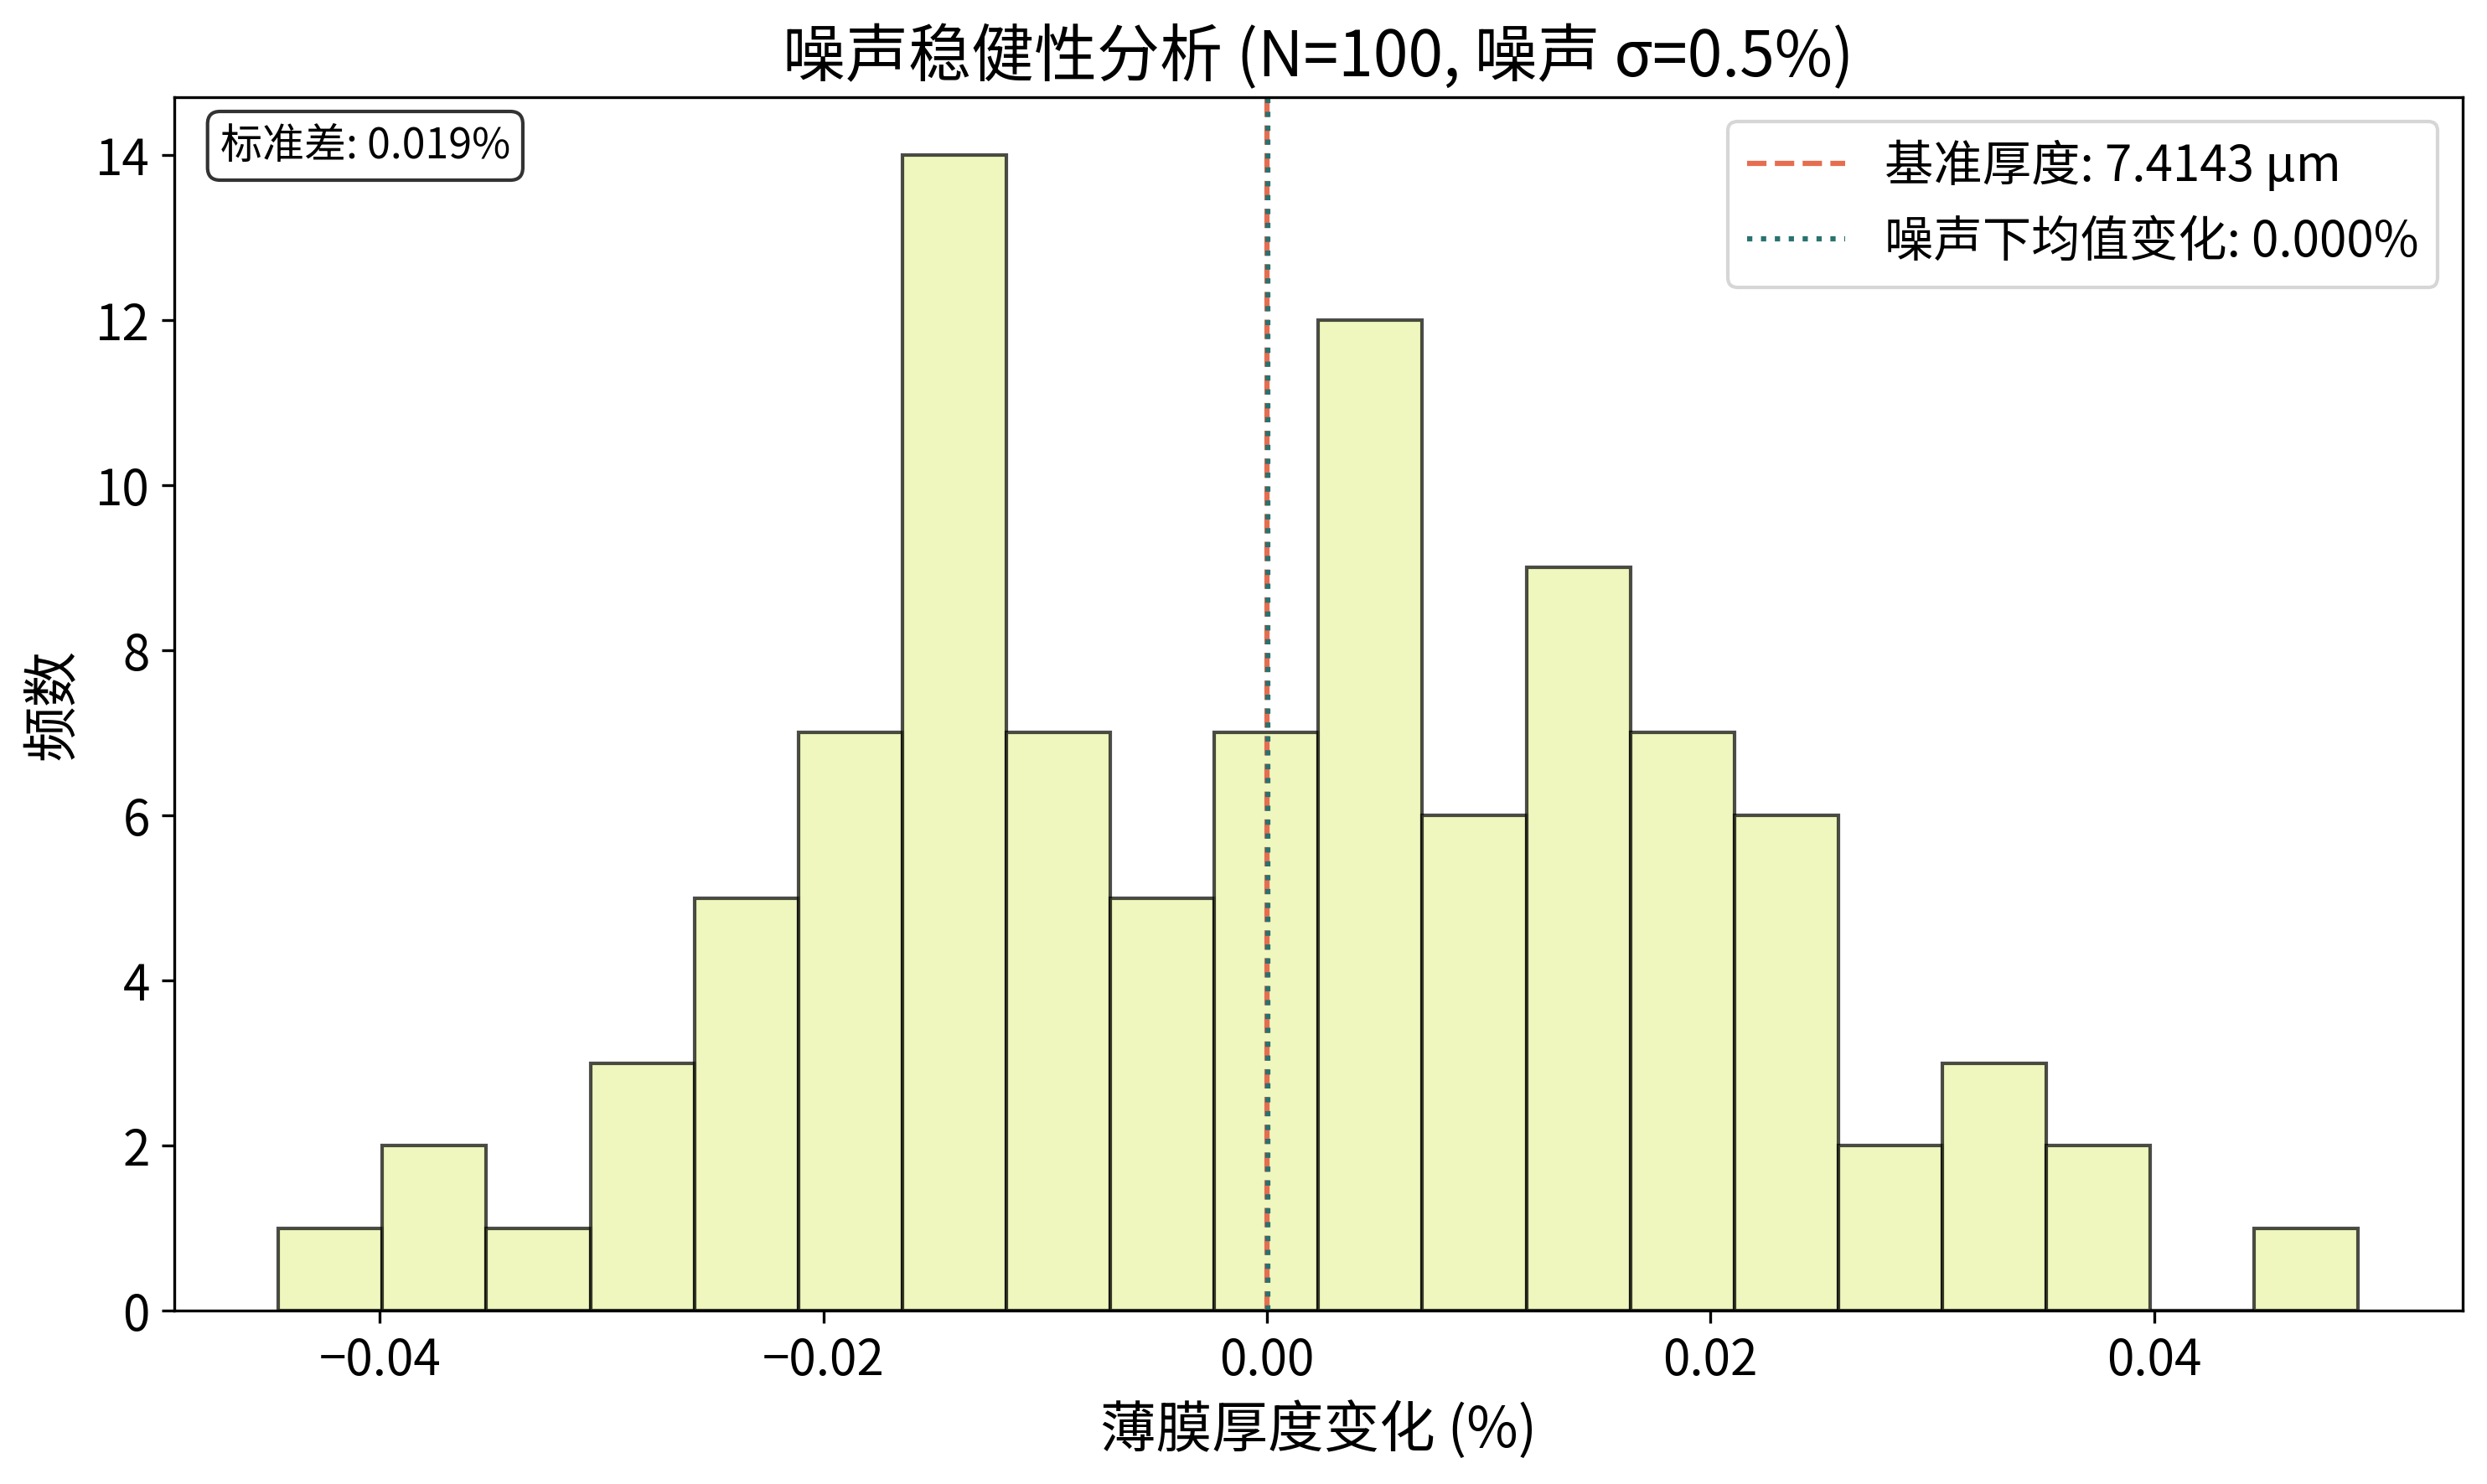
\includegraphics[width=0.5\textwidth]{问题二稳定性.png}
  \caption{FFT算法在随机噪声下的稳定性检验（蒙特卡洛模拟结果）}
  \label{fig:noise_robustness1}
\end{figure}

由结果统计直方图（\ref{fig:noise_robustness1}）可知，所有计算结果的均值变化率$<0.0001\%$，说明我们建立的基于双光束干涉和洛伦兹-德鲁德模型计算外延层厚度模型非常有效，能够对含有真实测量噪声的光谱数据进行精确分析。
\subsubsection{问题三基于傅里叶变换的计算外延层厚度方法稳定性}
类似于问题二的检验，我们对附件3的原始反射率数据叠加了标准差为0.5\%的高斯白噪声，重复200次，每次都使用带有不同随机噪声序列的数据，进行厚度计算。计算结果如\textbf{图（\ref{fig:noise_robustness}）}所示。

\begin{figure}[htbp]
  \centering
  % --- 请将 "噪声稳健性分析图.png" 替换为您图片的实际文件名 ---
  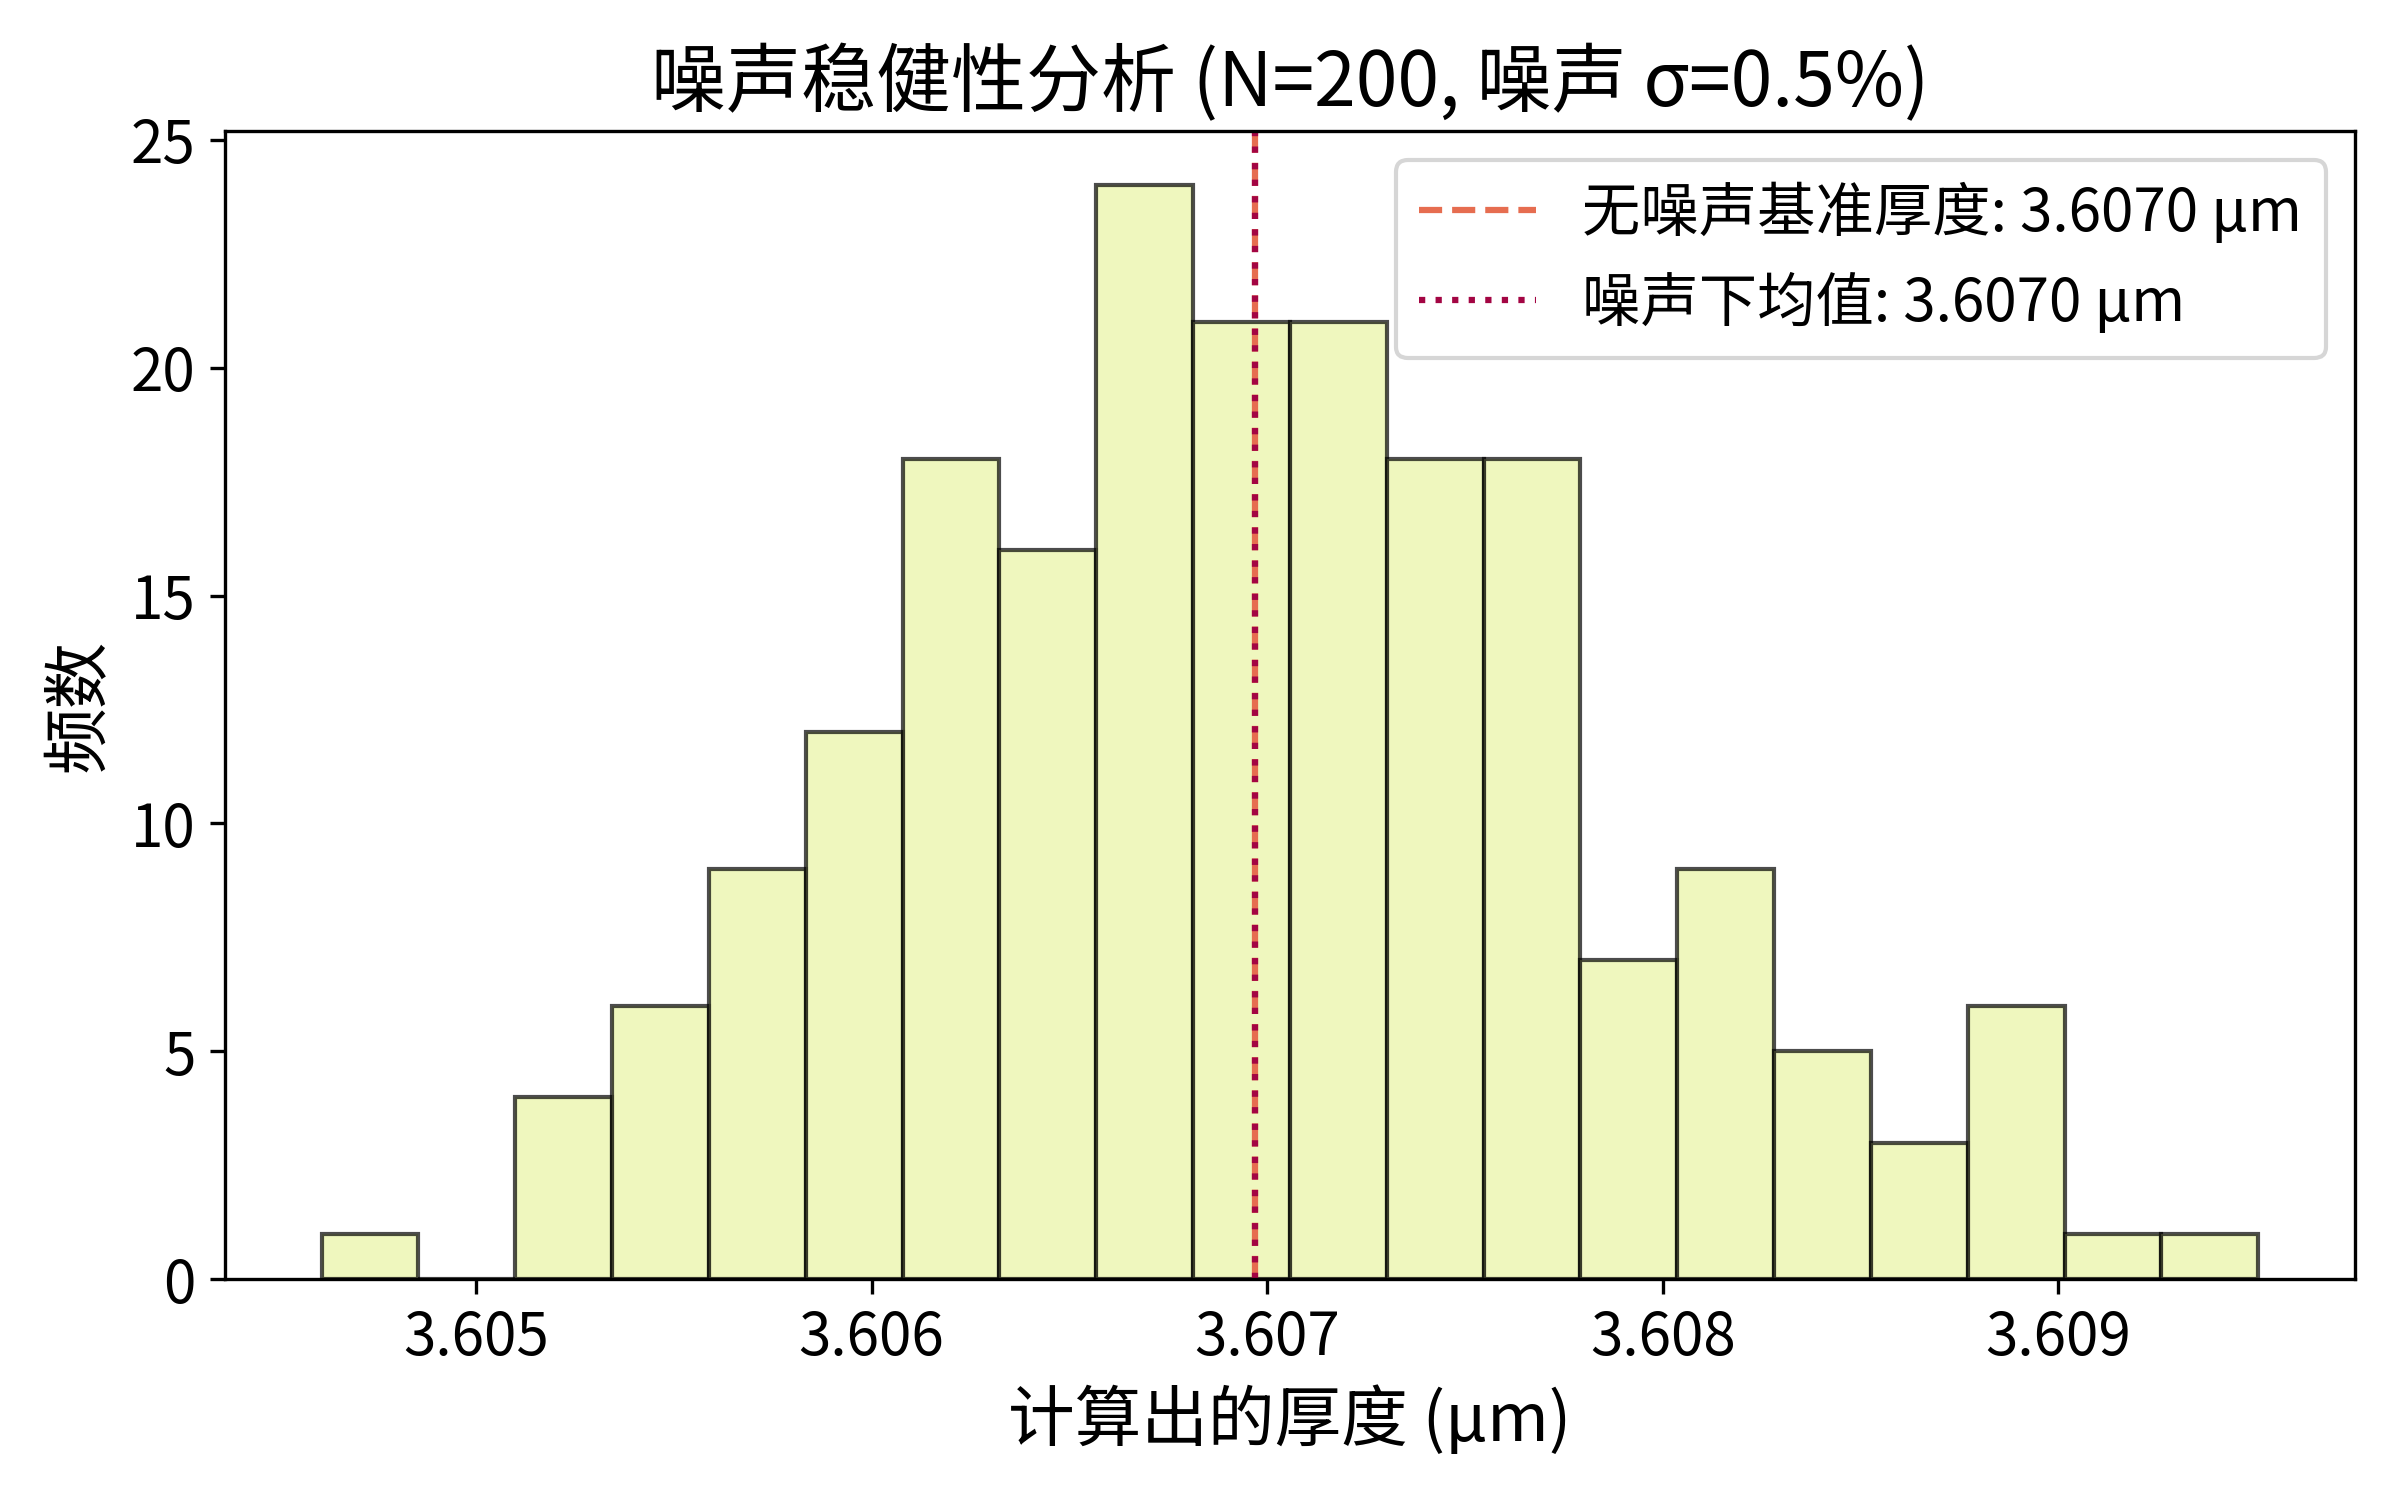
\includegraphics[width=0.5\textwidth]{稳定性.png}
  \caption{基于双光束干涉和洛伦兹-德鲁德模型计算外延层厚度方法在随机噪声下的稳定性检验（蒙特卡洛模拟结果）}
  \label{fig:noise_robustness}
\end{figure}

我们发现，所有计算值的均值（3.6070 $\mu m$，图中紫色虚线所示）与无噪声情况下的基准真值（3.6070 $\mu m$，图中红色虚线所示）相近。这充分表明，我们所建立的基于傅里叶变换的算法具有较好的噪声抑制能力。

\section{模型评价}
% (1) 对整个建模过程和结果进行评价。
% (2) 优点要说充分，缺点不回避。

\subsection{模型的优点}
\begin{enumerate}
    \item \textbf{物理模型解释性强：} 本文针对碳化硅和硅的不同材料特征，分别建立了基于洛伦兹-德鲁德模型和三项塞尔迈耶方程的物理模型，解释了光谱形成的物理机制，具有很高精度与实际价值。

    \item \textbf{算法策略精度高：} 
    针对问题二，我们采用了“全局同步拟合”策略和“差分进化+局部优化”的先进算法，有效避免了局部最优解，保证了结果的全局最优性。
    针对问题三，我们创新性地引入了带色散校正的傅里叶变换法，通过坐标变换有效地解决了FFT的系统误差问题。

    \item \textbf{结果可靠性高：} 本文不仅给出了计算结果，还通过多种手段对其可靠性进行了交叉验证。例如，通过计算折射率验证了双光束模型的合理性；通过对比不同角度的计算结果验证了一致性；通过灵敏度和稳定性分析（蒙特卡洛模拟）全面检验了模型的鲁棒性。

    % \item \textbf{针对性强，实用价值高：} 针对碳化硅和硅两种不同光学特性的材料，我们分别设计了最优的建模与求解方案，使得模型兼具高精度与高效率，具有很强的实际应用价值。
\end{enumerate}

\subsection{模型的缺点}
\begin{enumerate}
    \item \textbf{标准洛伦兹-德鲁德模型对高掺杂衬底的描述不佳：} 在问题二中，残差分析显示，模型在“剩余射线带”存在系统性偏差。这反映，标准的洛伦兹-德鲁德模型可能未能完全捕捉到高度掺杂半导体中声子与等离激元之间的复杂耦合效应。
    \item \textbf{对碳化硅材质的假设局限性：}问题二中假设碳化硅是标准的4H-SiC材料，而实际上工业生产的碳化硅晶圆可能存在多种晶型，例如6H-SiC或3C-SiC，它们具有不同的晶格结构，这将直接导致其本征光学参数不同。此假设引入了系统性误差。
    \item \textbf{复杂拟合中的参数耦合风险：} 在问题二的七参数全局拟合的逆问题中，存在参数耦合的固有挑战——理论上可能存在另一组略有不同的参数组合，也能产生非常相似的拟合光谱。
    \item \textbf{对固定参数精确性的依赖：}问题二的固定洛伦兹-德鲁德模型参数，以及问题三的三项塞尔迈耶方程参数，其精度都高度依赖于文献所给参数的准确性。文献中的标准值可能与实际样品的真实光学常数存在微小差异。
\end{enumerate}

\subsection{模型的改进}
\begin{enumerate}
    \item \textbf{引入声子-等离激元耦合模型代替标准洛伦兹-德鲁德模型：}
    根据文献\cite{shokhovets2011infrared}，在高载流子浓度的碳化硅中，声子和等离激元会发生强烈的耦合。我们可以采用文献中一个统一的\textbf{LO声子-等离激元耦合模型}来描述介电函数，来减少在“剩余射线带”观察到的系统性拟合偏差。
    \item \textbf{拉曼光谱法进行晶型无损鉴定：}为了解决碳化硅晶型不确定导致系统误差的问题，我们可以先对样品进行拉曼光谱无损检测，鉴定出样品准确晶型，再为该晶型选取对应的正确光学本征参数代入红外光谱模型。
    \item \textbf{采用贝叶斯推断优化算法：}
    为了解决复杂拟合中解的不唯一性，可以采用基于\textbf{马尔可夫链蒙特卡洛}的贝叶斯分析框架\cite{arregui2019bayesian}，此算法能够探索整个参数空间，并给出每个参数的后验概率分布。
\end{enumerate}


%==========================================================================
%   参考文献
%==========================================================================
% \bibliographystyle{gbt7714-numerical} % 由 gbt7714 宏包自动设置样式，此处重复声明会导致 BibTeX “another \bibstyle command” 报错，故注释

\bibliography{cite}        





%==========================================================================
%   附录
%==========================================================================
\appendix
\newpage
\section{支撑材料文件列表}
\begin{itemize}
    \item \texttt{q2.py}: 用于问题二模型求解的核心Python代码。
    \item \texttt{q3-interfere.py}: 用于问题三基于干涉极值点求解的核心Python代码。
    \item \texttt{q3-fft.py}: 用于问题三基于色散矫正傅里叶变换求解的核心Python代码。
    \item \texttt{q2-verification}: 问题二模型稳定性检验。
    \item \texttt{sensitivity.py}: 用于检验问题二、三模型的灵敏度。
    \item \texttt{AI工具使用详情说明.pdf}: AI工具使用详情说明。
\end{itemize}

% --- 如果没有支撑材料，请取消下面一行的注释 ---
% \noindent 本论文没有需要提供的支撑材料。

\section{主要源程序代码}

% --- 如果没有用到程序，请取消下面一行的注释 ---
% \noindent 本论文没有用到程序。

\subsection{问题二求解的 Python 关键代码 (q2.py)}
\lstinputlisting[language=Python, caption={问题二求解核心代码}]{code/q2.py}
% 注意：请确保您的代码文件 (例如 main_q1.py) 与 main.tex 在同一目录下。
% 如果代码不长，也可以直接写在下面：
% \begin{lstlisting}[language=Python, caption={问题一求解核心代码}]
% import numpy as np
% 
% def solve_q1():
%     # 这里是你的代码
%     print("Hello, MCM!")
%     return True
%
% if __name__ == '__main__':
%     solve_q1()
% \end{lstlisting}
\subsection{问题三干涉极值求解的 Python 关键代码 (q3-interfere.py)}
\lstinputlisting[language=Python, caption={问题三求解核心代码}]{code/q3-interfere.py}
\subsection{问题三基于色散矫正傅里叶变换求解的 Python 关键代码 (q3-fft.py)}
\lstinputlisting[language=Python, caption={问题三求解核心代码}]{code/q3-fft.py}



% \section{其他附录内容}
% % (1) 某一问题的详细证明或求解过程
% % (2) 自己在网上找到的数据
% % (3) 比较大的流程图
% % (4) 较繁杂的图表或计算结果

% [此处可以添加更多附录内容...]

\end{document}
%--------------------------------------------------------------------------
%   文档结束
%--------------------------------------------------------------------------